%
A fit using data is performed on using bins which are not blinded. The bins with S/B ratio of greater than 5\% are blinded in both pre-fit and post-fit yield plots. The signal sample is not included in the fit (it is a background-only fit). The blinded fit provides information on the modeling agreement in background-dominated regions of phase space, and systematics can be pulled from their initial value as well as constrained.

The blinded data fit is performed over all control and signal regions, and with all available samples and systematics. The dominant ttbar background is reweighted using the NN method.

The post-fit distributions associated with each background and signal region are shown in Figure \ref{fig:Postfit_Yields_1L} for 1L regions and Figure \ref{fig:Postfit_Yields_2L} for 2LOS regions from the combined fit using mass point $m_H=400$ GeV. The nuisance parameter pulls and constraints are compared between 1L, 2LOS, and the combined fit in Figures \ref{fig:data_NP_instrumental}, \ref{fig:data_NP_ttbar}, and \ref{fig:data_NP_other}. Comparison for the fits using GNN outputs trained on various mass points are shown in Figures \ref{fig:data_NP_mass_instrumental}, \ref{fig:data_NP_mass_ttbar}, and \ref{fig:data_NP_mass_other}.

Correlation matrices for systematics for 1L, 2LOS, and the combined fit are shown in Figure \ref{fig:Corr_mH400_Data_1L}, Figure \ref{fig:Corr_mH400_Data_2L}, and Figure \ref{fig:Corr_mH400_Data_all} respectively.

\begin{figure}[htbp!]
        \begin{center} \setlength{\tabcolsep}{2.5pt}\footnotesize
        \begin{tabular}{cccc}
        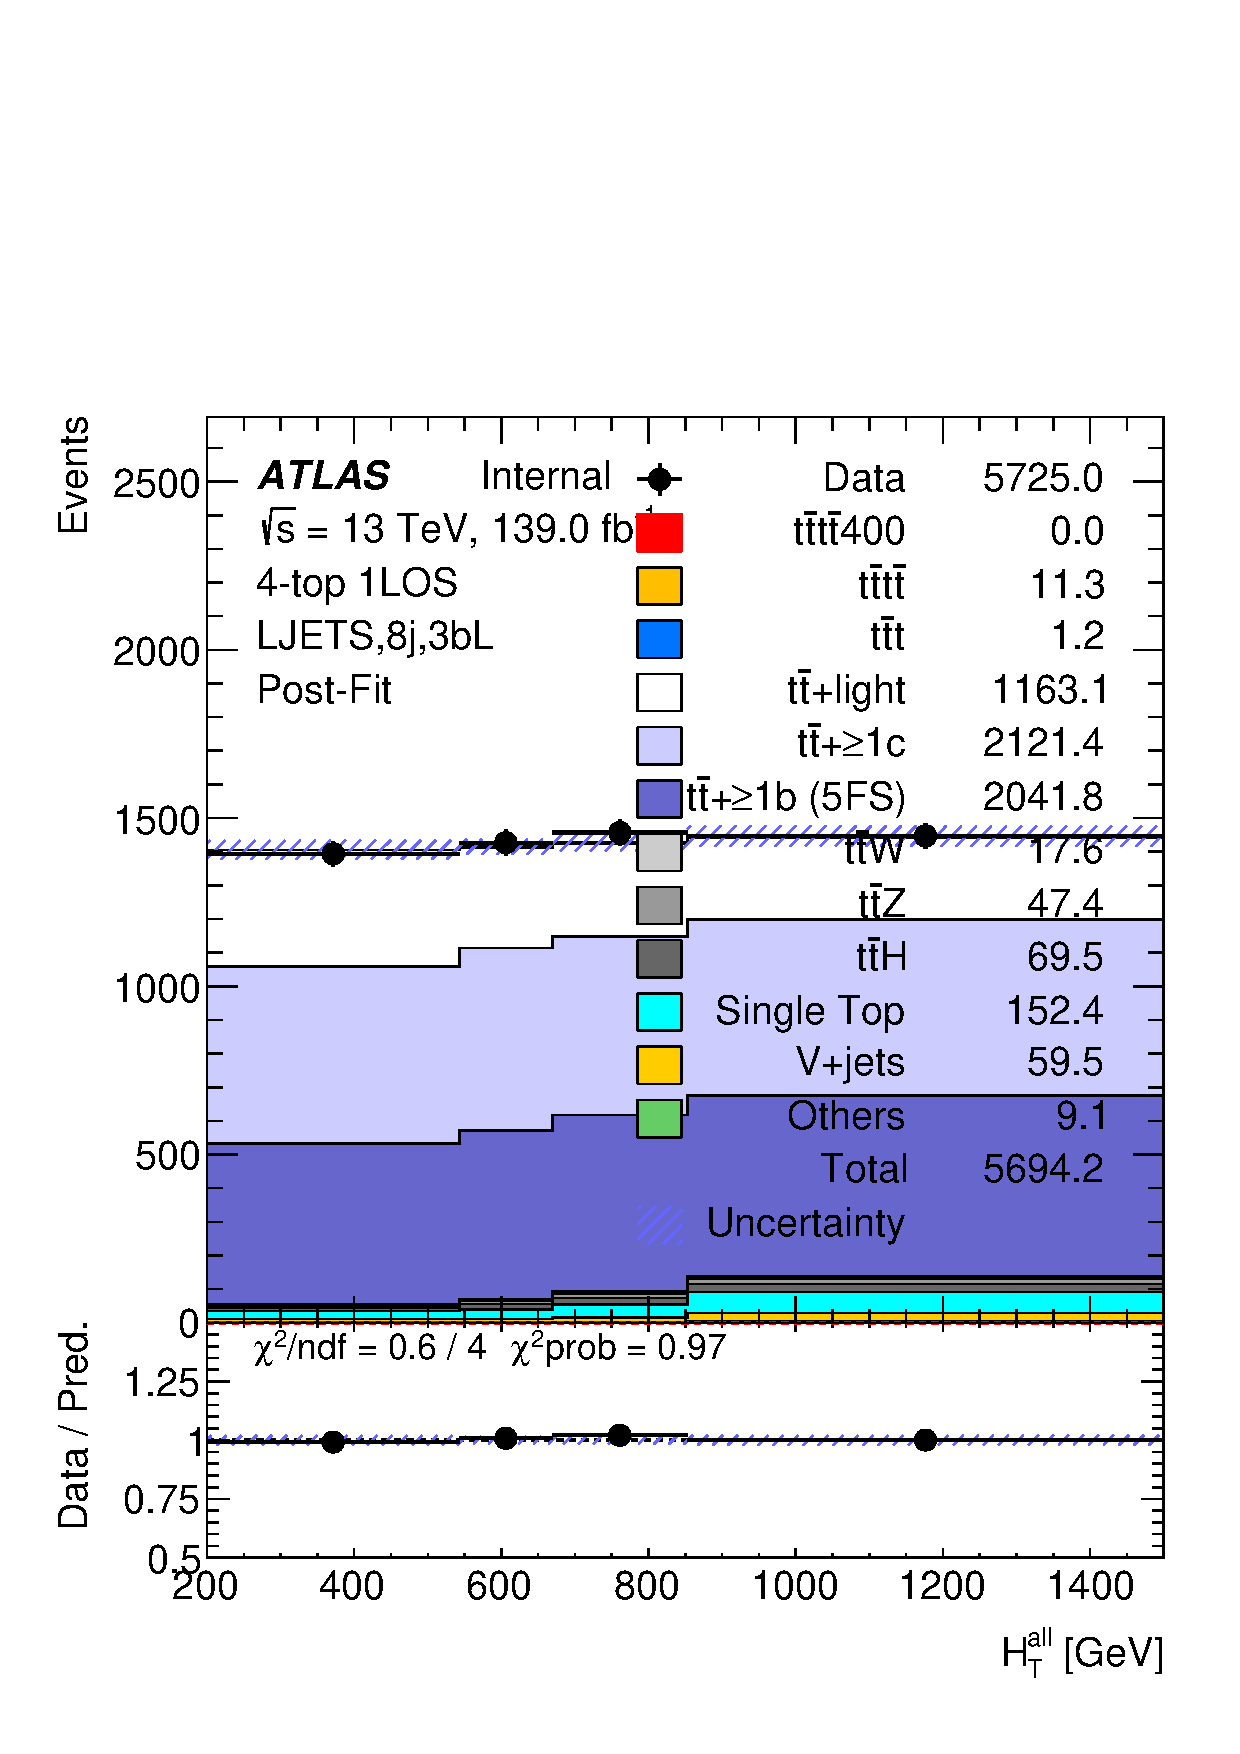
\includegraphics[width=0.23 \textwidth]{figures/fits/GNN/400/all/data/Plots/ljets_8j3bL_postFit.pdf} &
        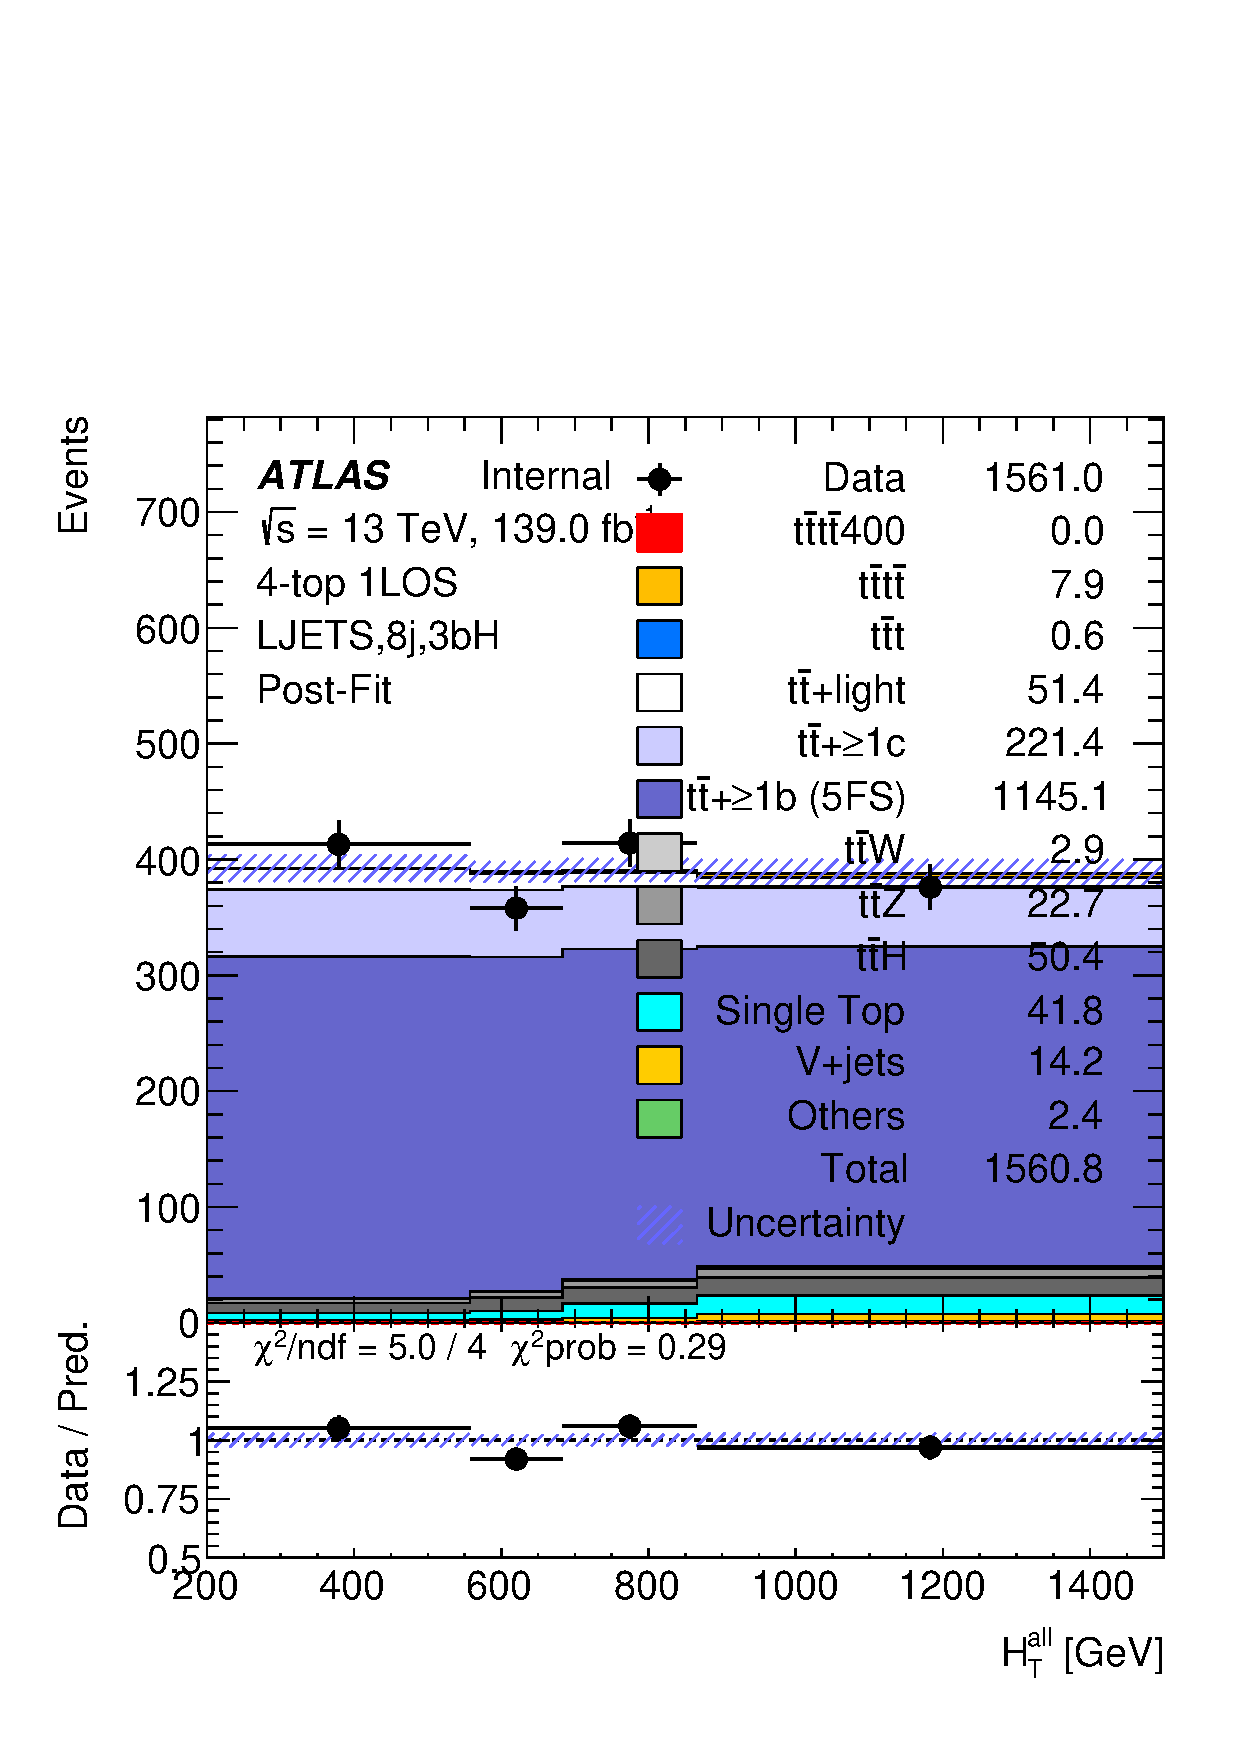
\includegraphics[width=0.23 \textwidth]{figures/fits/GNN/400/all/data/Plots/ljets_8j3bH_postFit.pdf} &
        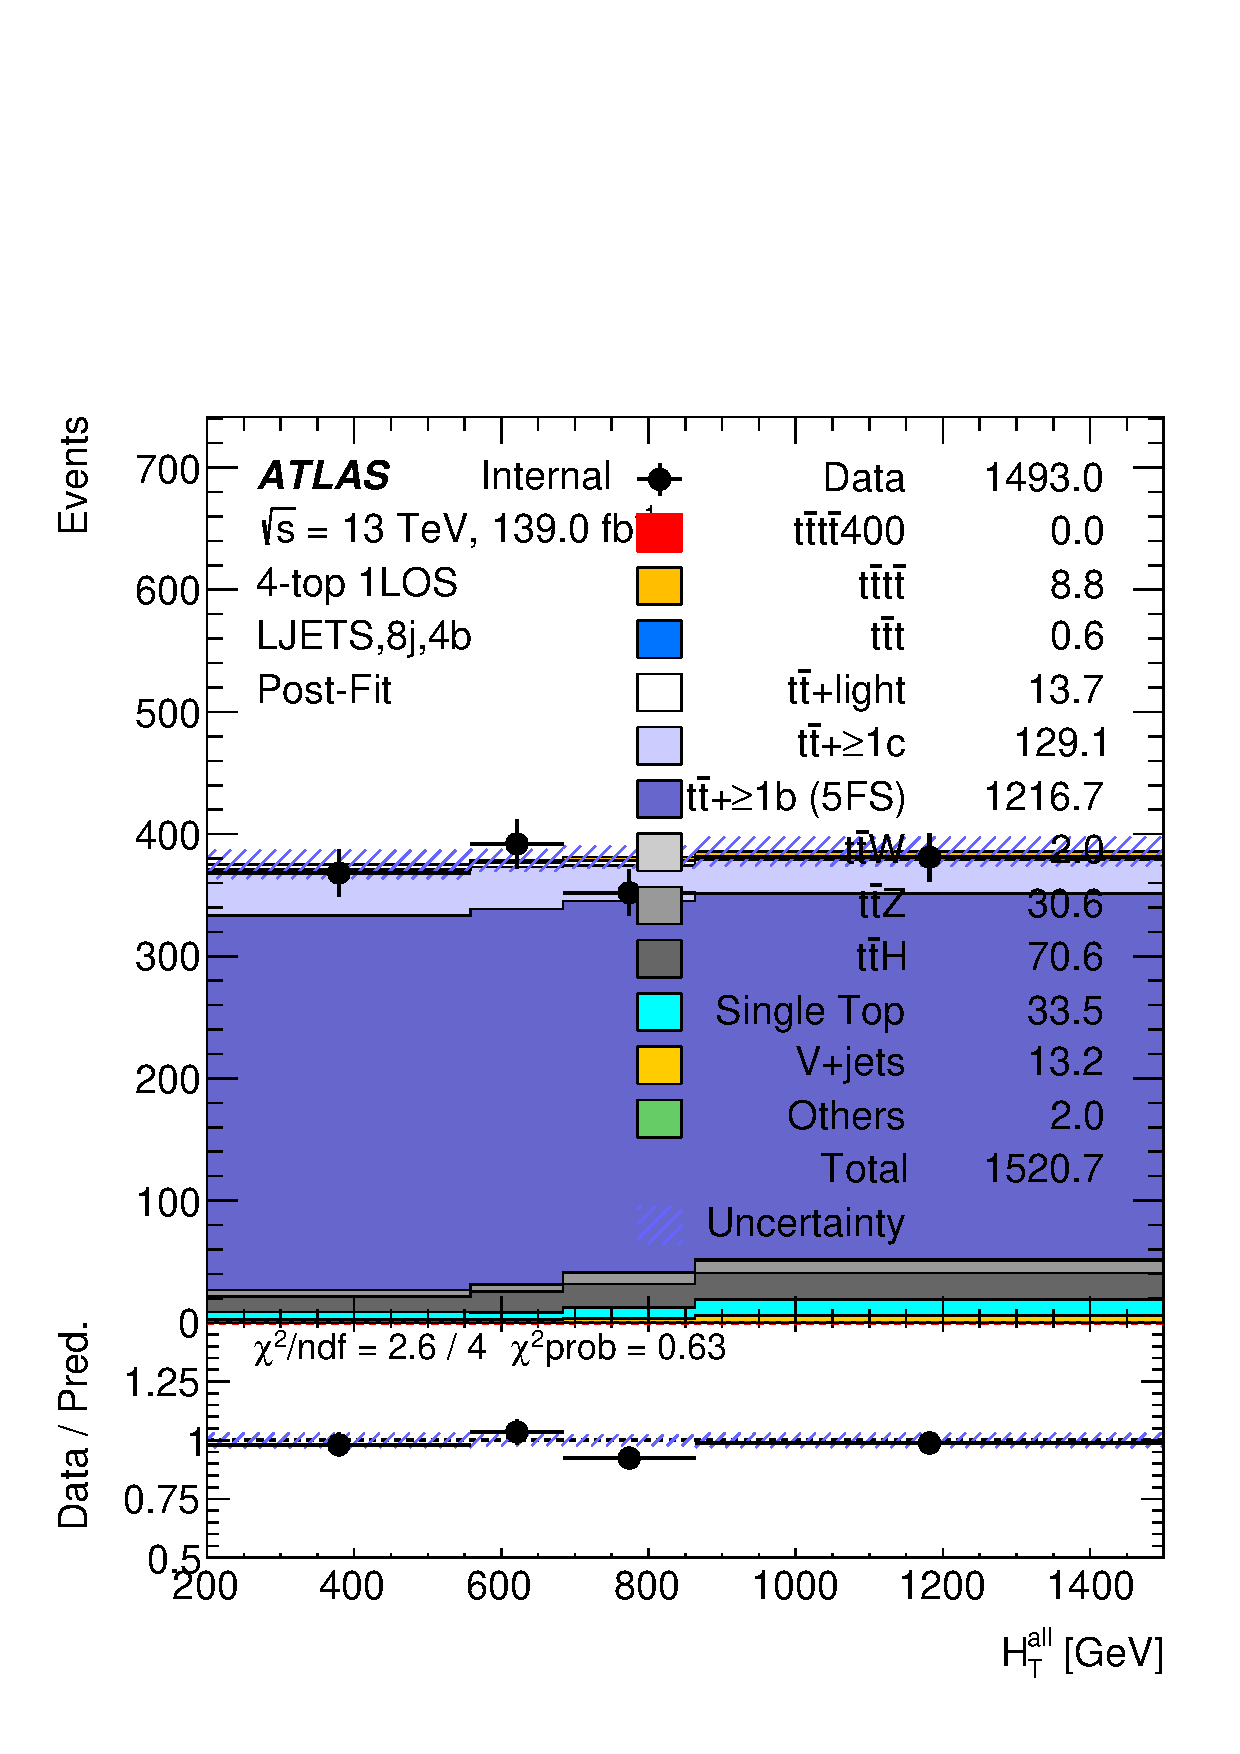
\includegraphics[width=0.23 \textwidth]{figures/fits/GNN/400/all/data/Plots/ljets_8j4b_postFit.pdf} &
        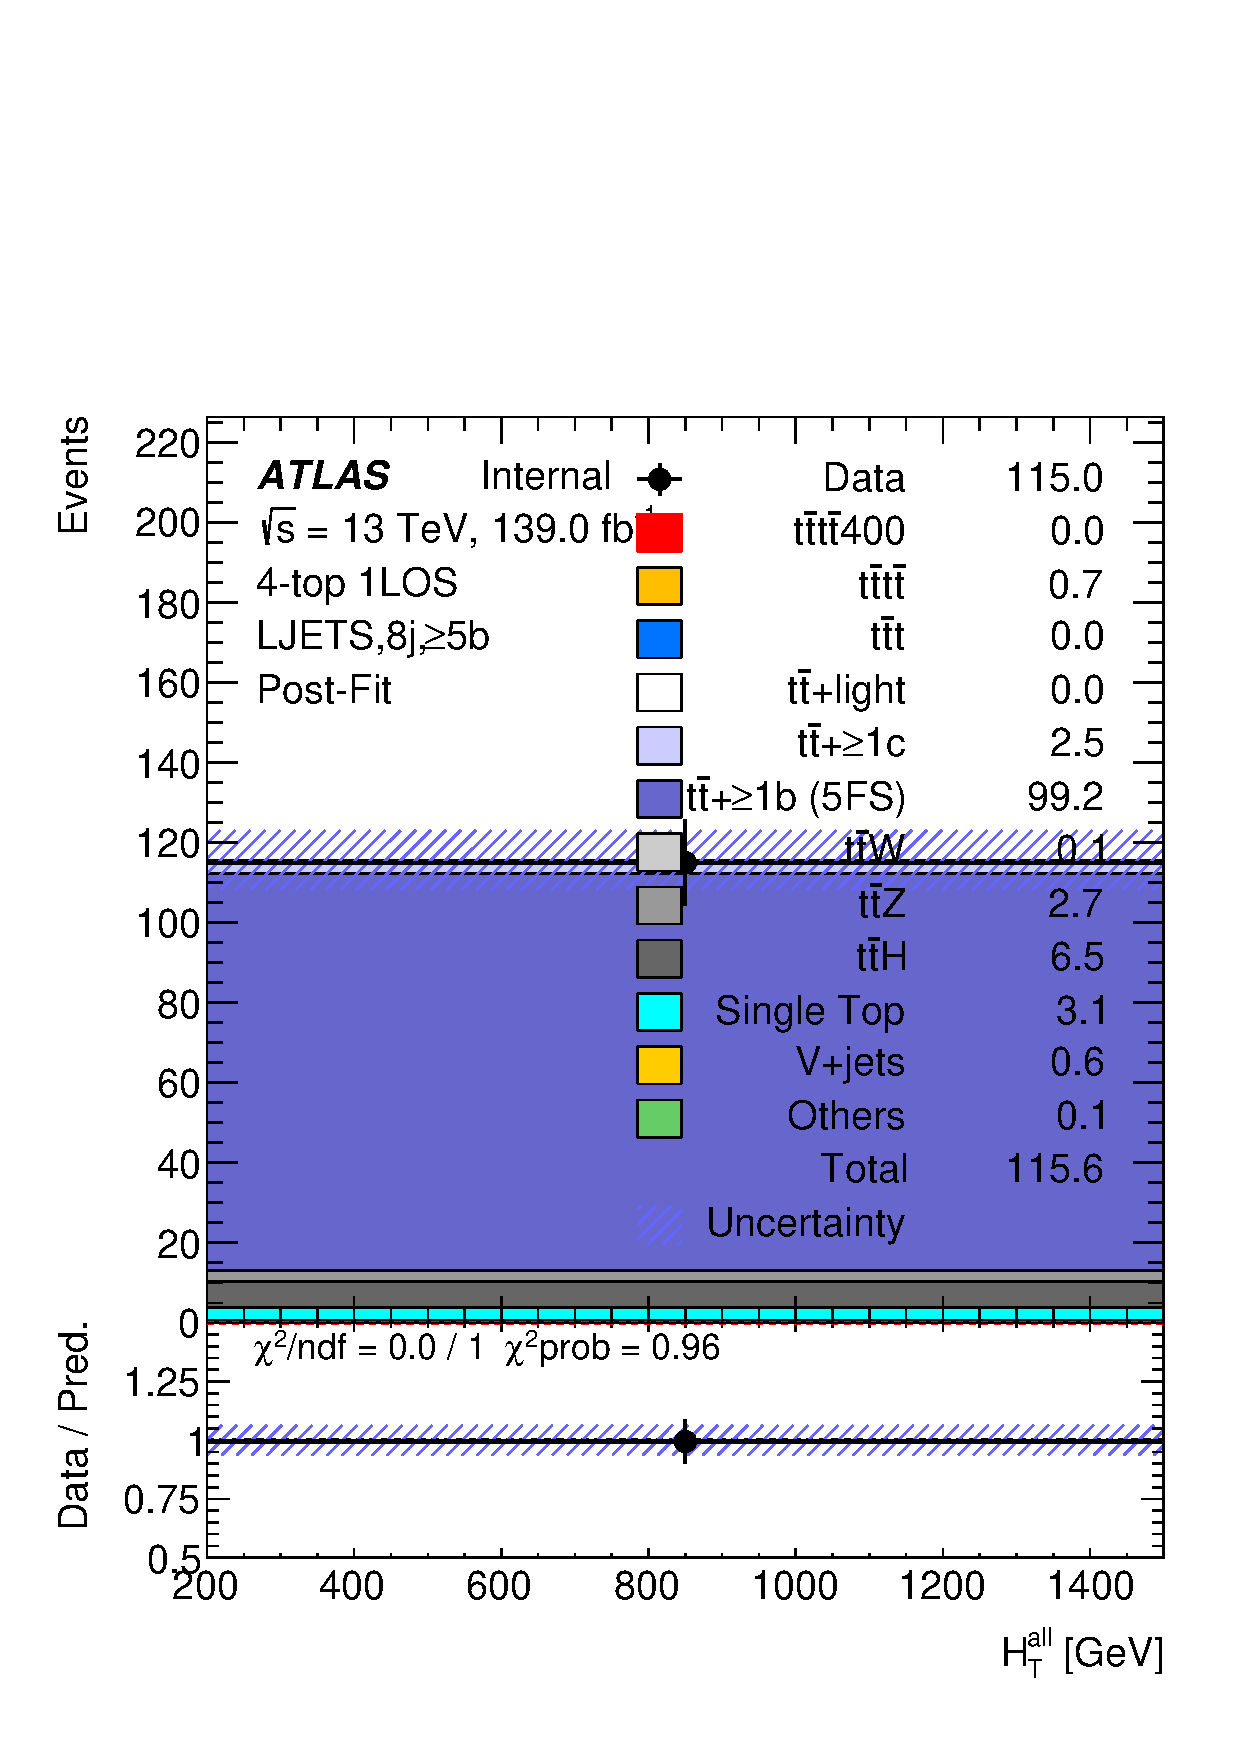
\includegraphics[width=0.23 \textwidth]{figures/fits/GNN/400/all/data/Plots/ljets_8jge5b_postFit.pdf}\\

        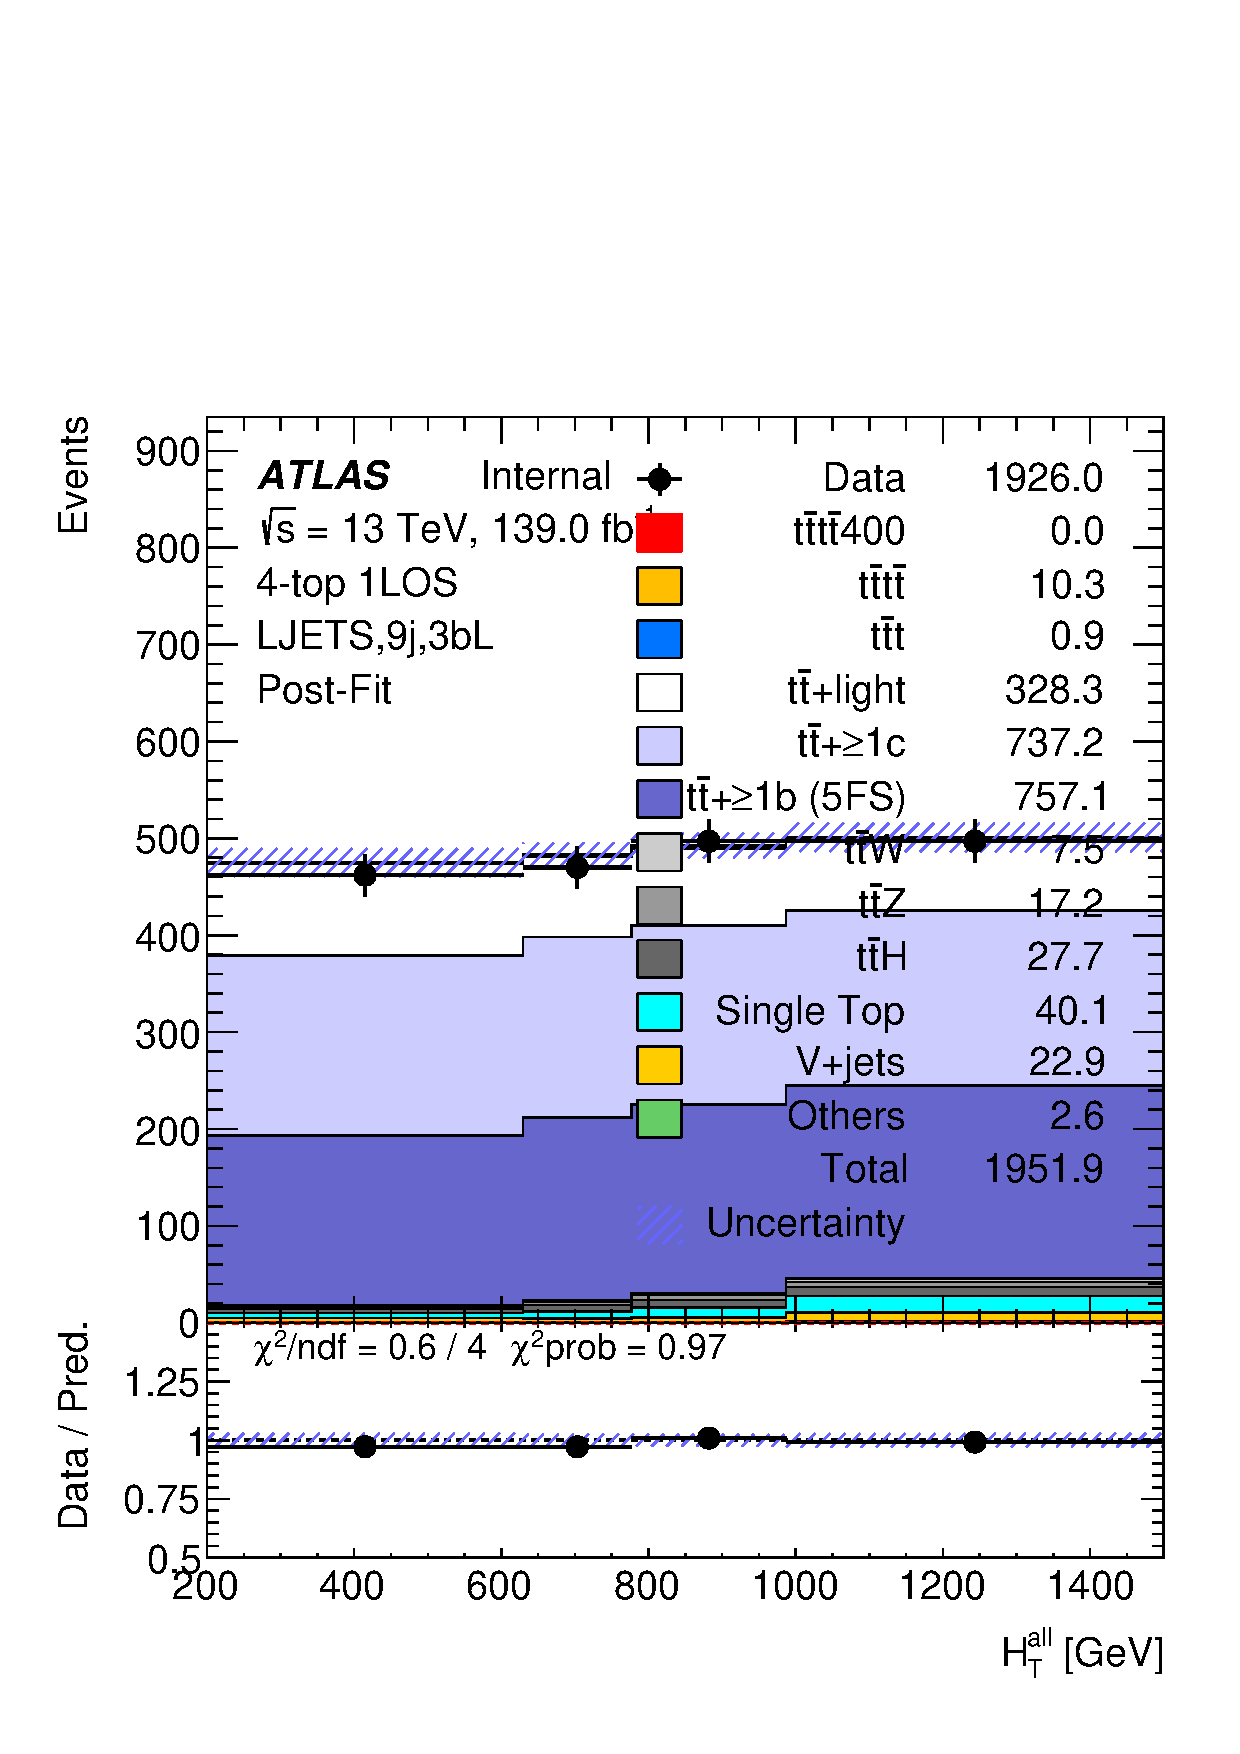
\includegraphics[width=0.23 \textwidth]{figures/fits/GNN/400/all/data/Plots/ljets_9j3bL_postFit.pdf} &
        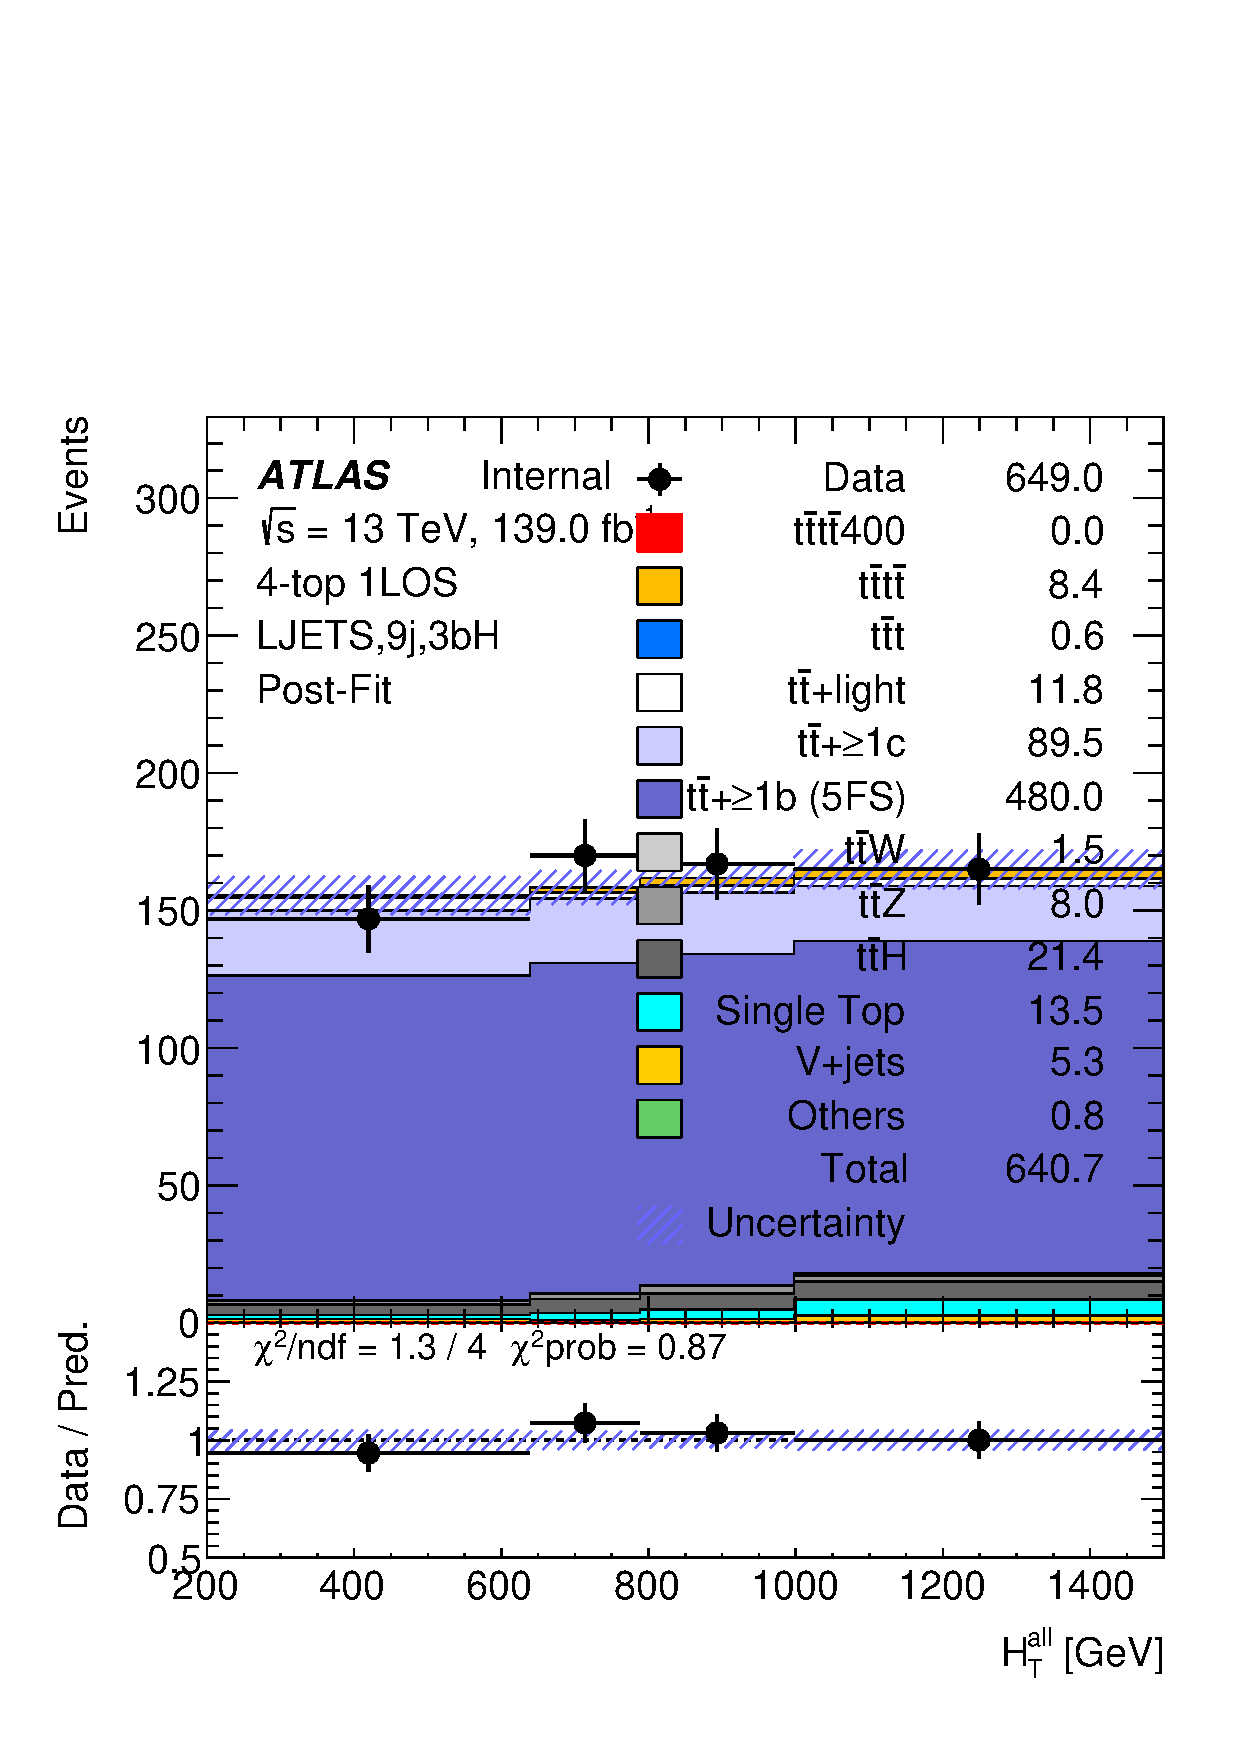
\includegraphics[width=0.23 \textwidth]{figures/fits/GNN/400/all/data/Plots/ljets_9j3bH_postFit.pdf} &
        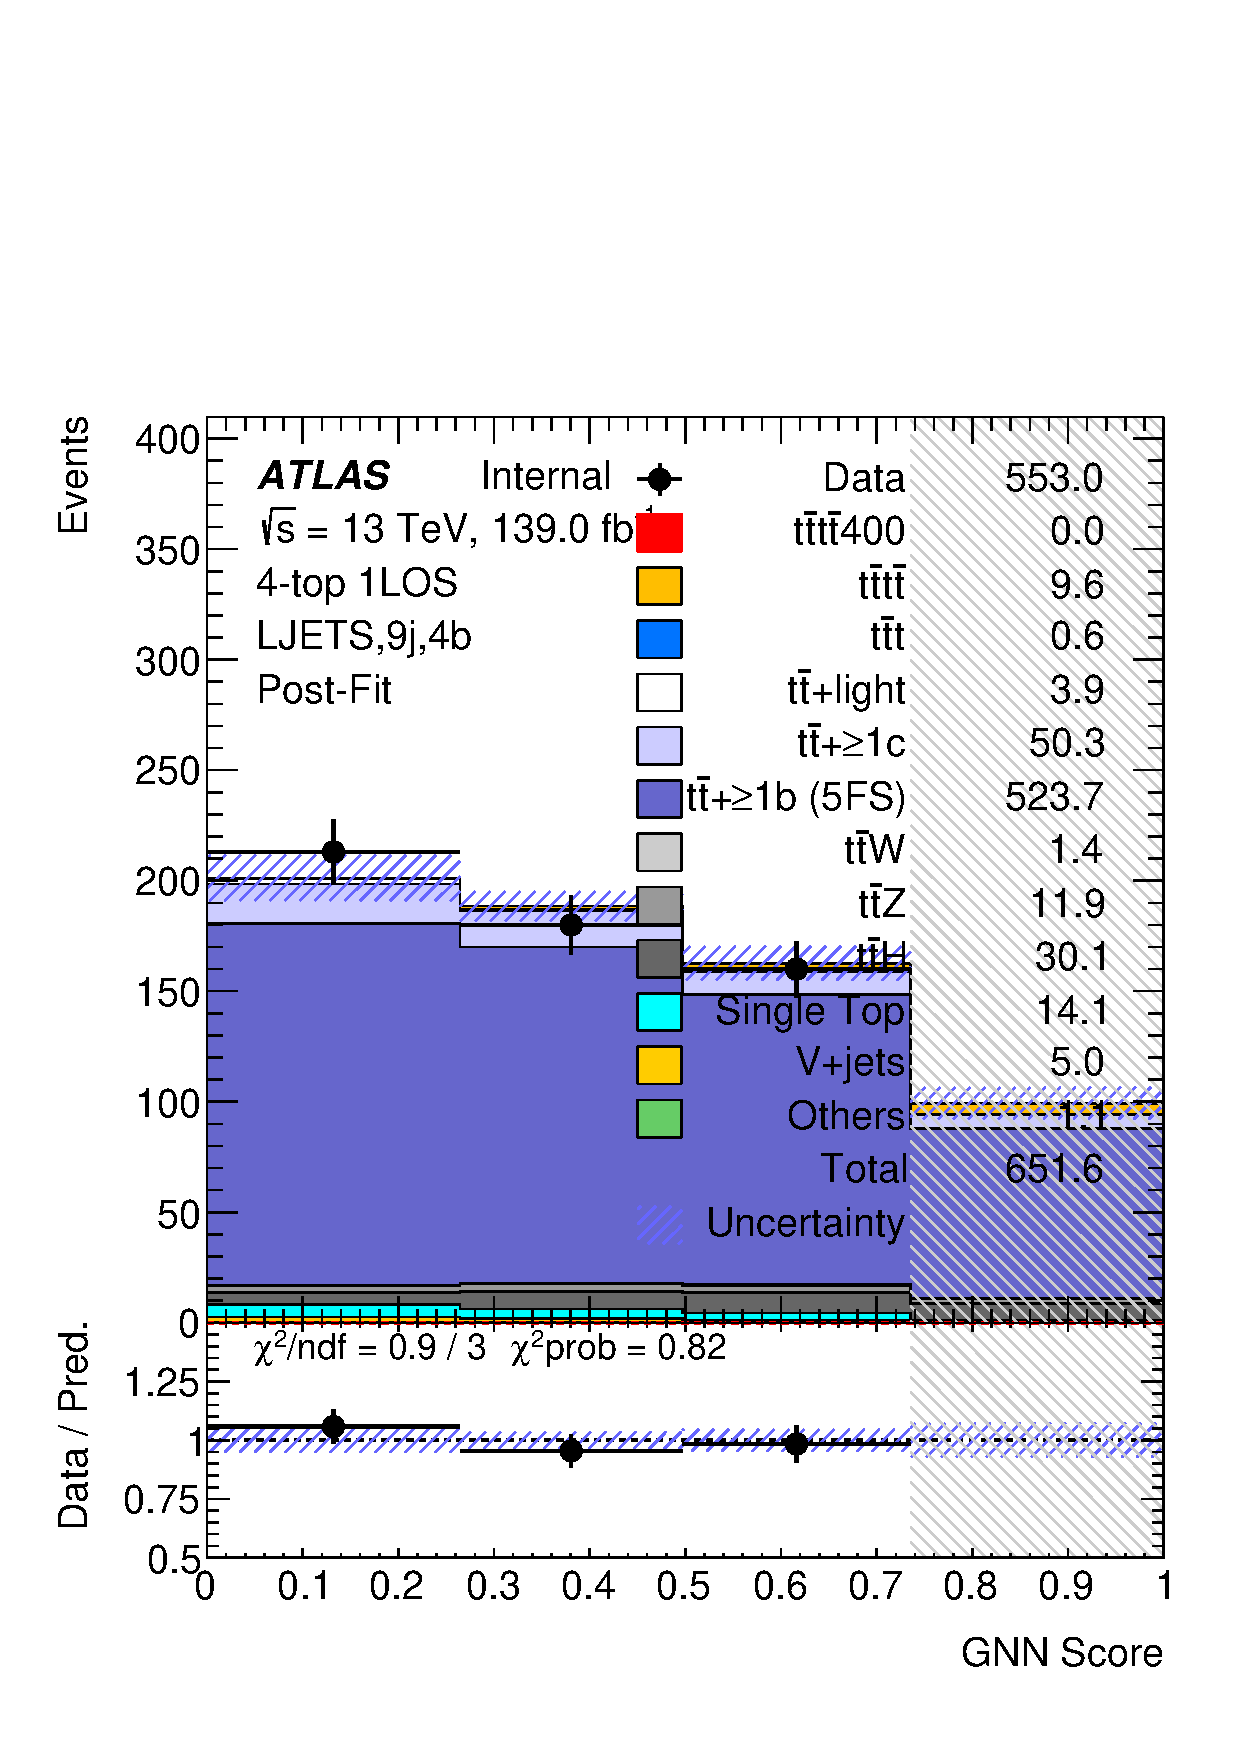
\includegraphics[width=0.23 \textwidth]{figures/fits/GNN/400/all/data/Plots/ljets_9j4b_postFit.pdf} &
        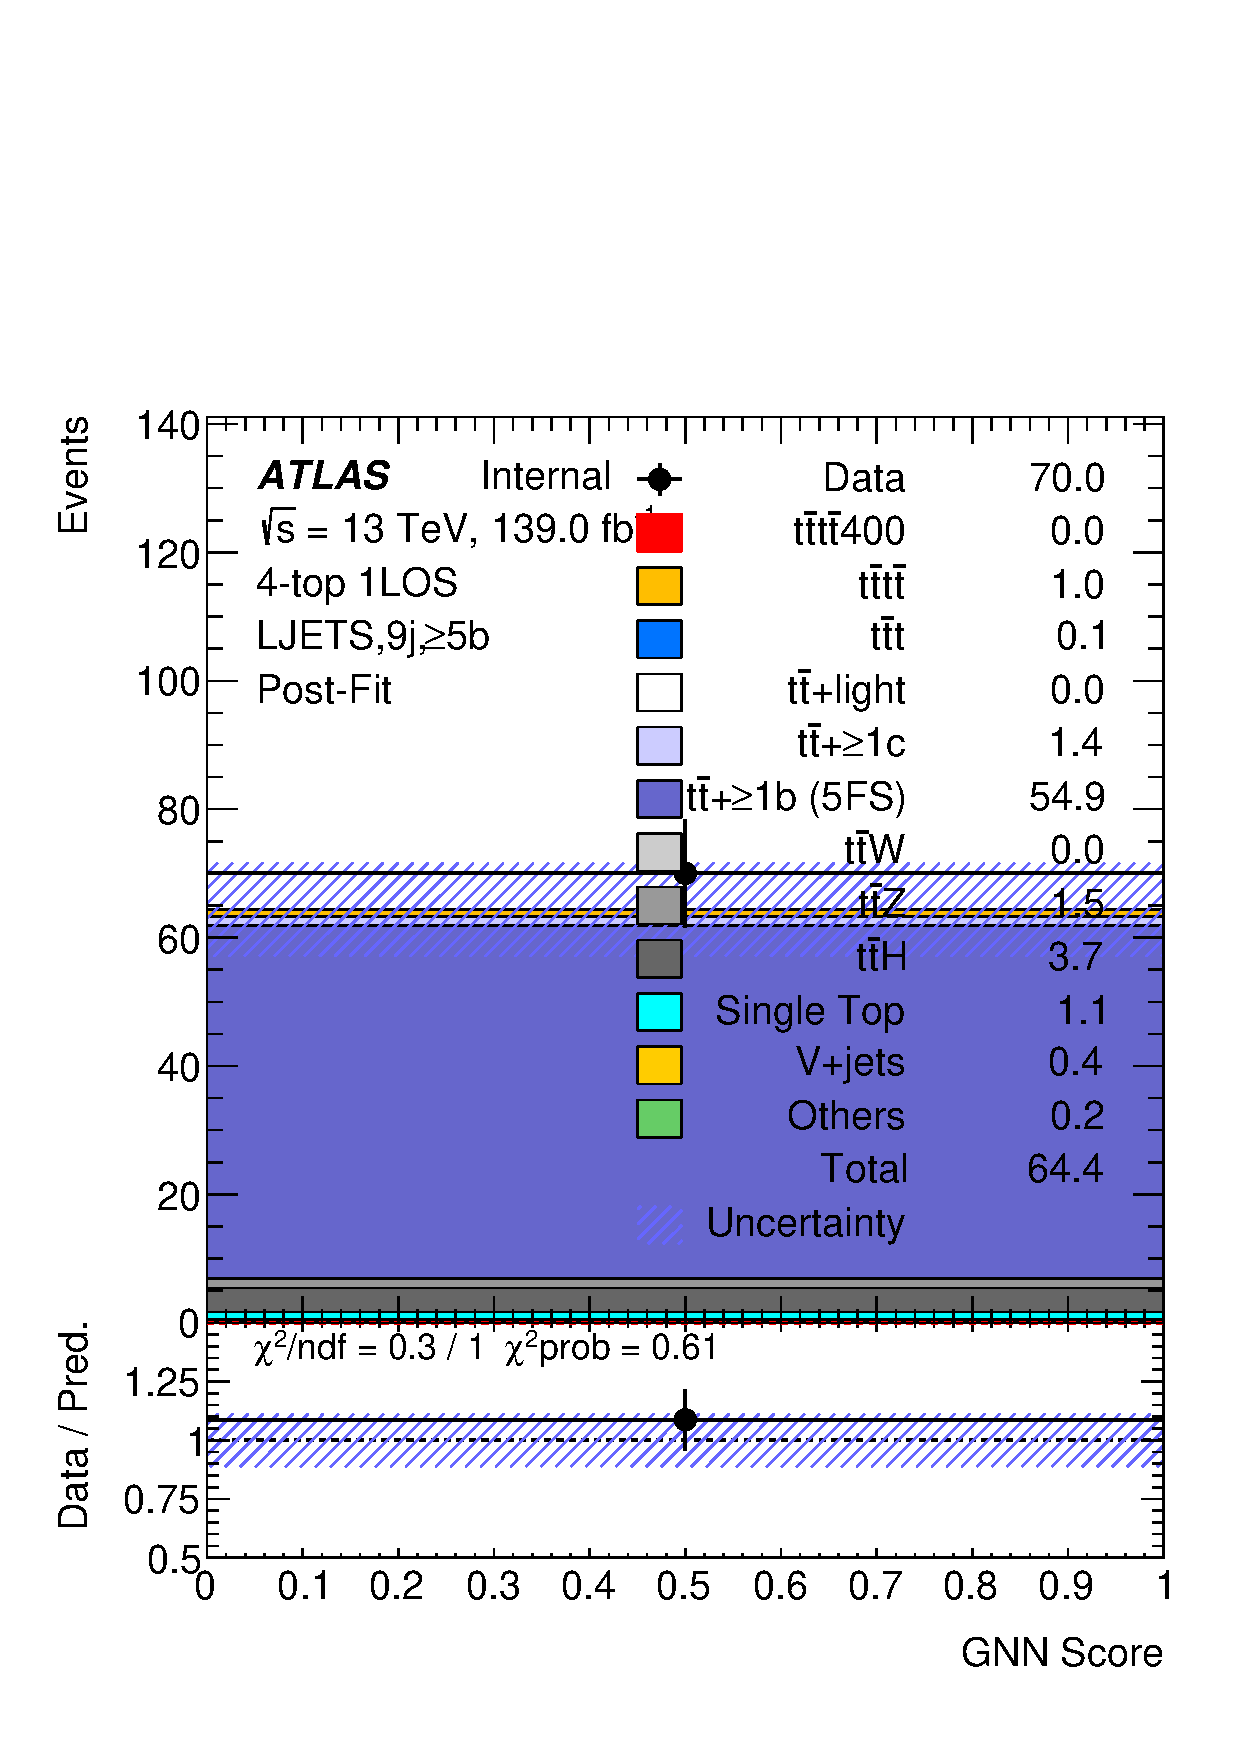
\includegraphics[width=0.23 \textwidth]{figures/fits/GNN/400/all/data/Plots/ljets_9jge5b_postFit.pdf} \\

        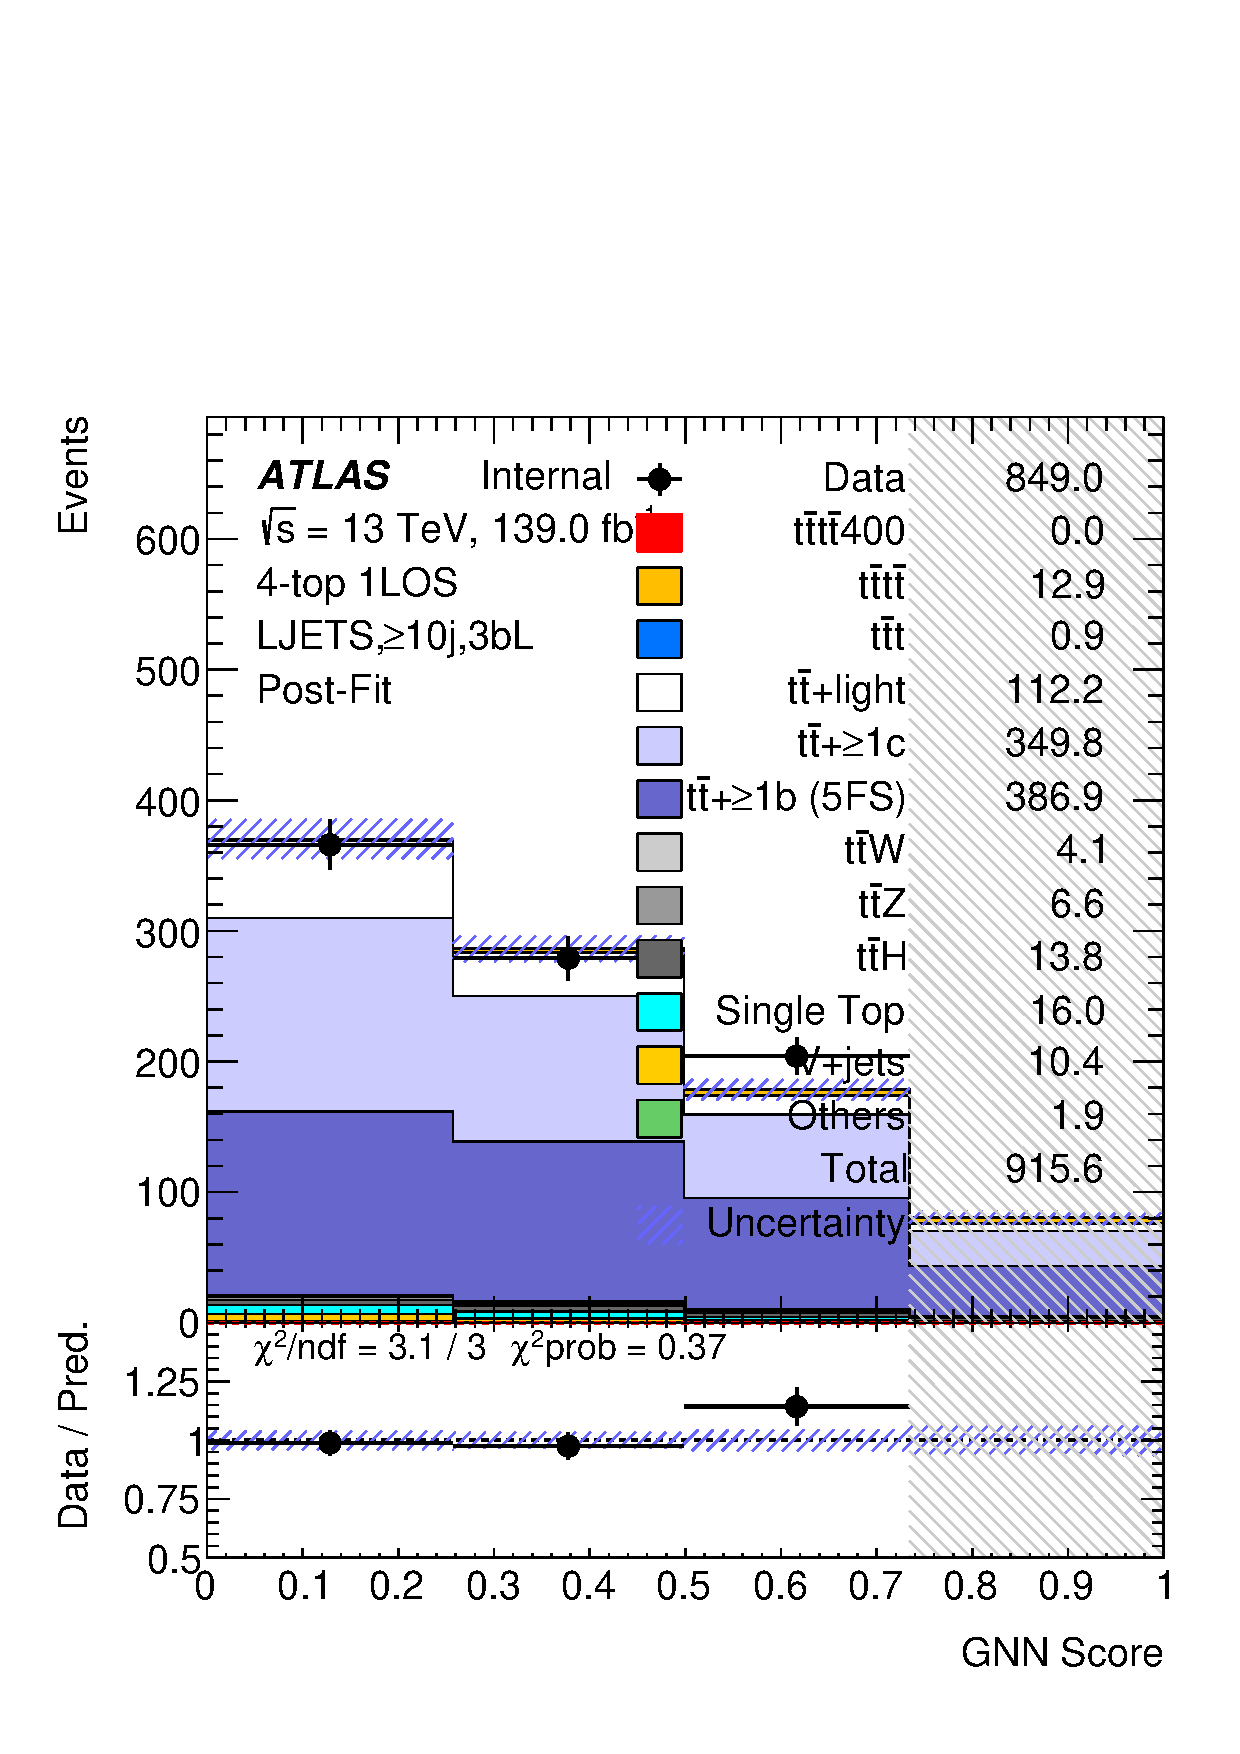
\includegraphics[width=0.23 \textwidth]{figures/fits/GNN/400/all/data/Plots/ljets_ge10j3bL_postFit.pdf} &
        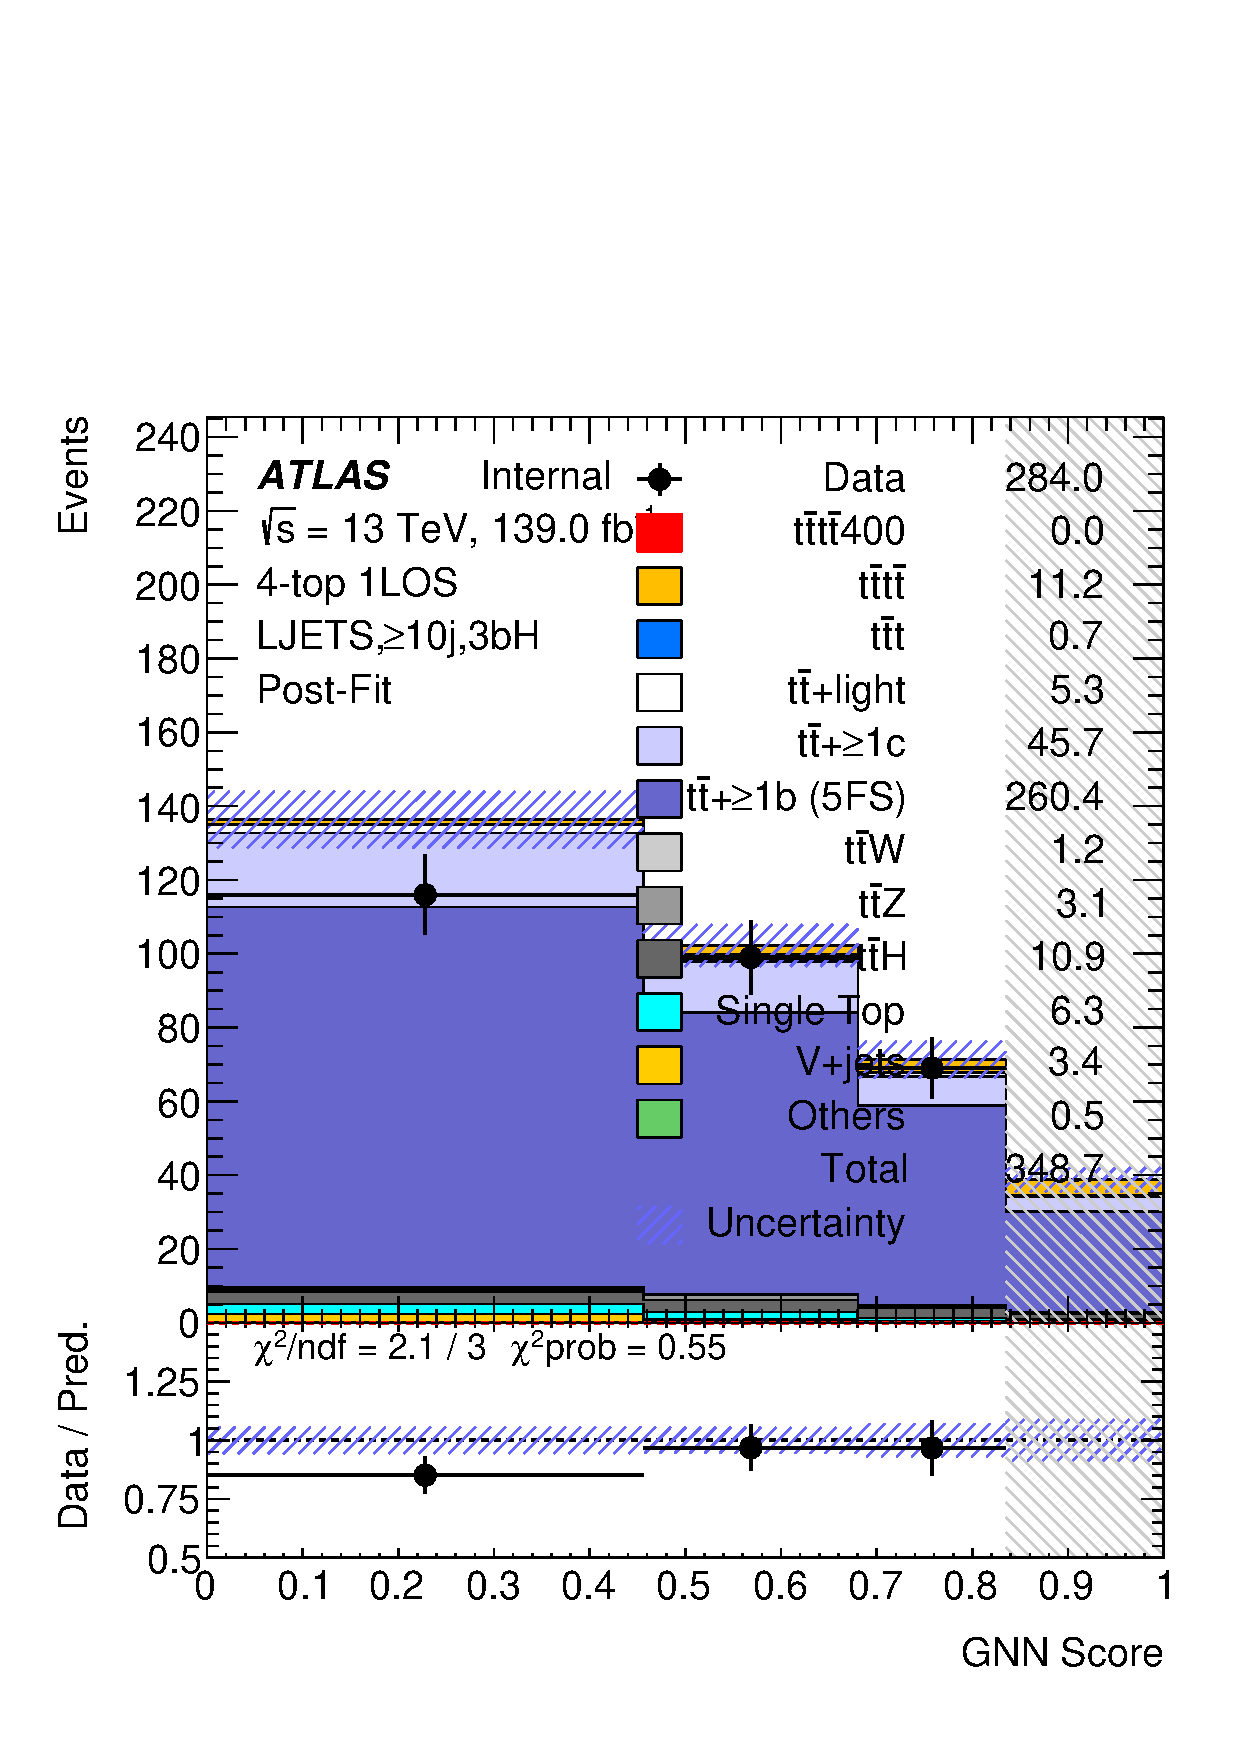
\includegraphics[width=0.23 \textwidth]{figures/fits/GNN/400/all/data/Plots/ljets_ge10j3bH_postFit.pdf} &
        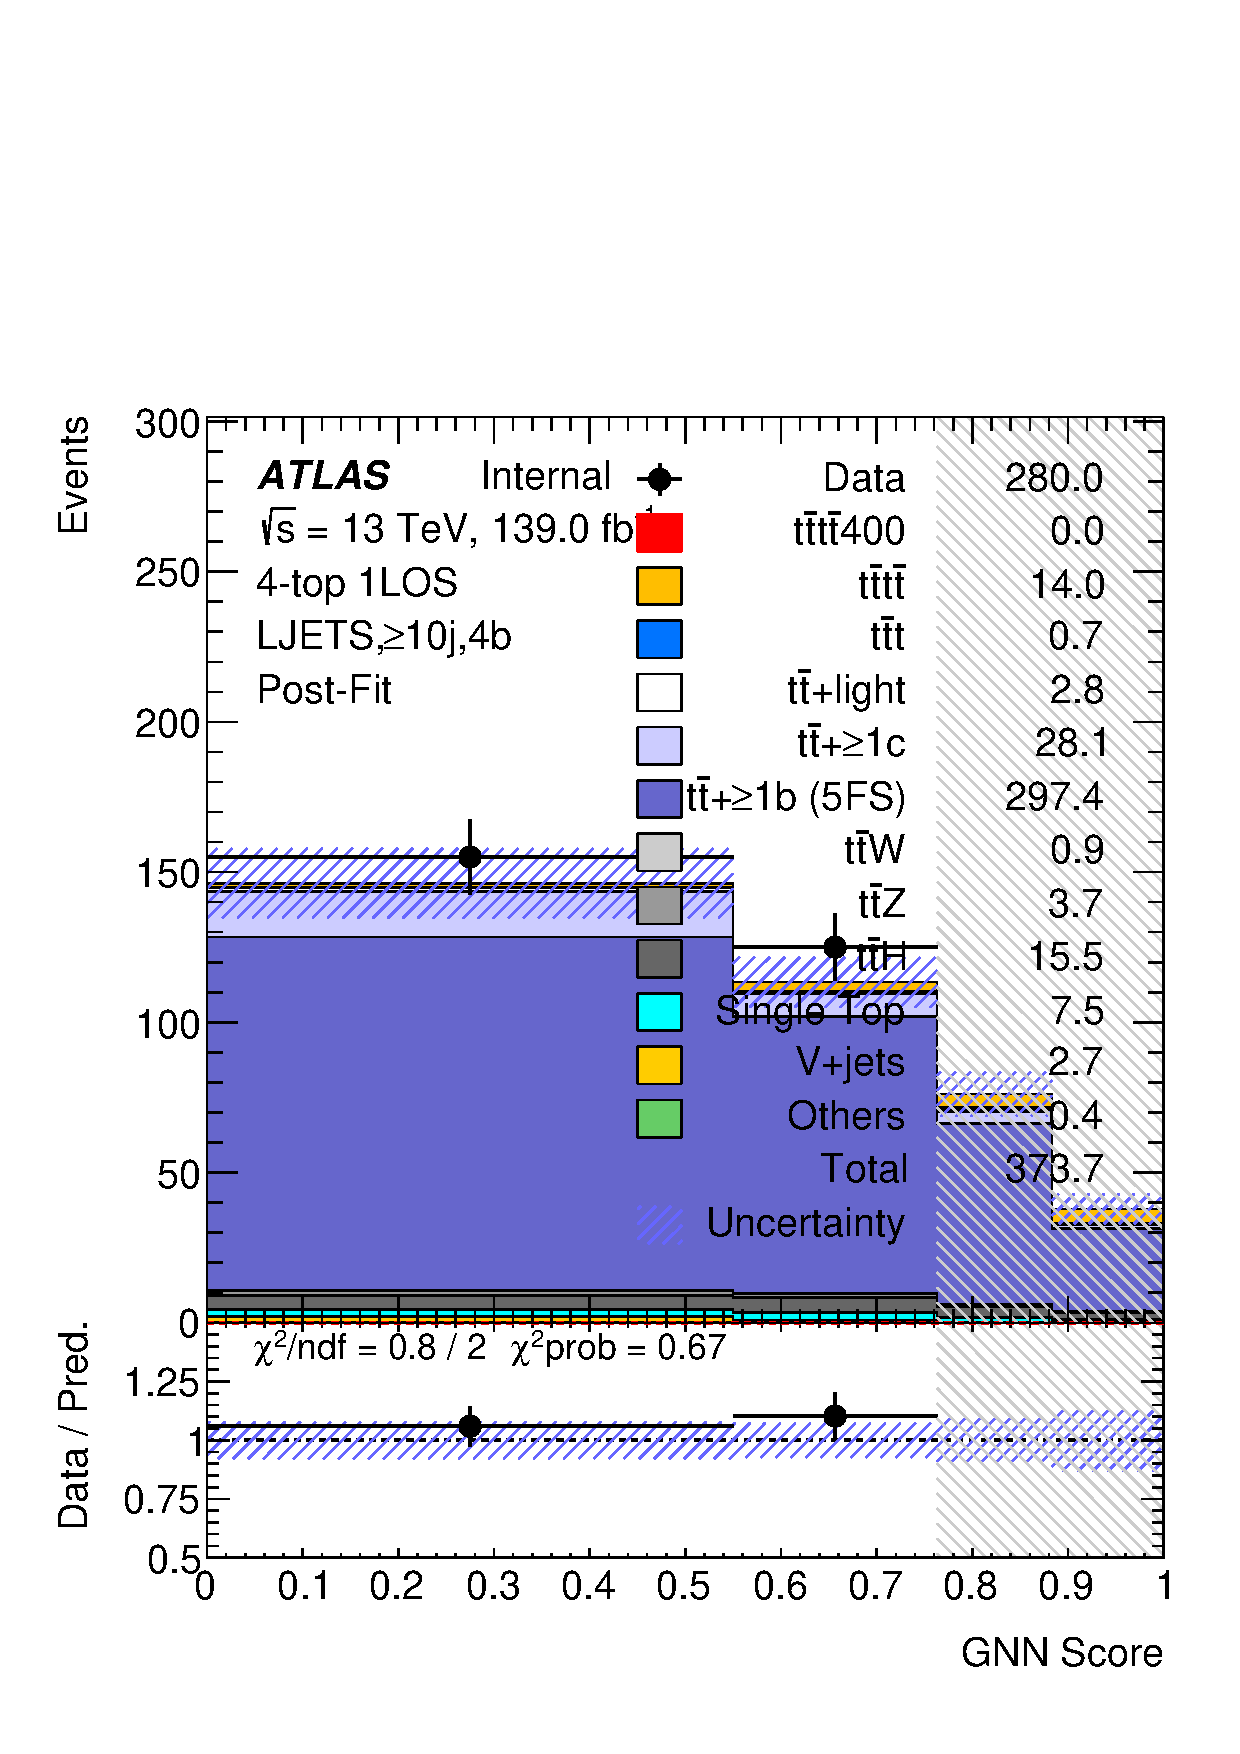
\includegraphics[width=0.23 \textwidth]{figures/fits/GNN/400/all/data/Plots/ljets_ge10j4b_postFit.pdf} &
        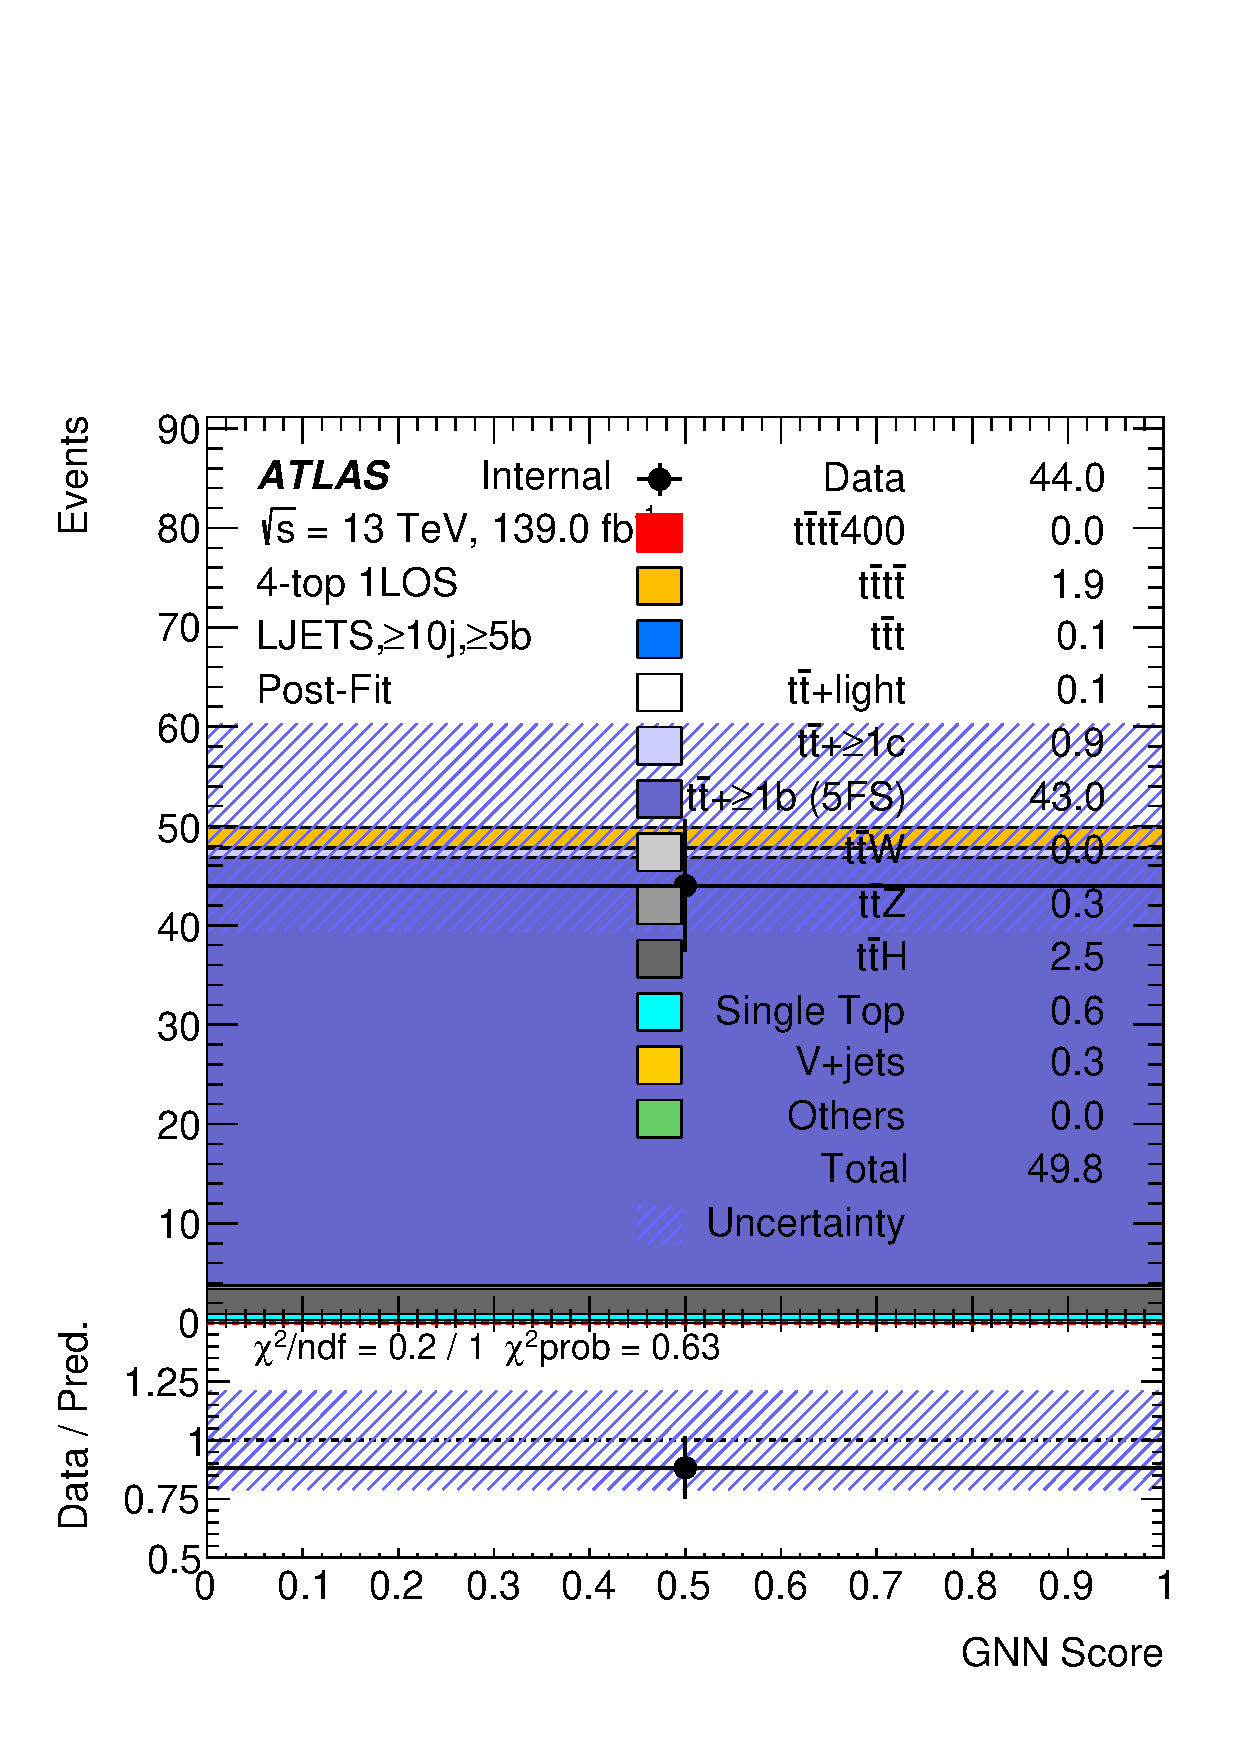
\includegraphics[width=0.23 \textwidth]{figures/fits/GNN/400/all/data/Plots/ljets_ge10jge5b_postFit.pdf} \\
        \end{tabular}
        \caption{\label{fig:Postfit_Yields_1L}Post-fit distributions for 1L regions associated with different signal and background samples, compared with data yields for mH = 400 GeV. The fit is done using all regions (1L+2L).}
\end{center}
\end{figure}

\begin{figure}[htbp!]
        \begin{center} \setlength{\tabcolsep}{2.5pt}\footnotesize
        \begin{tabular}{ccc}
        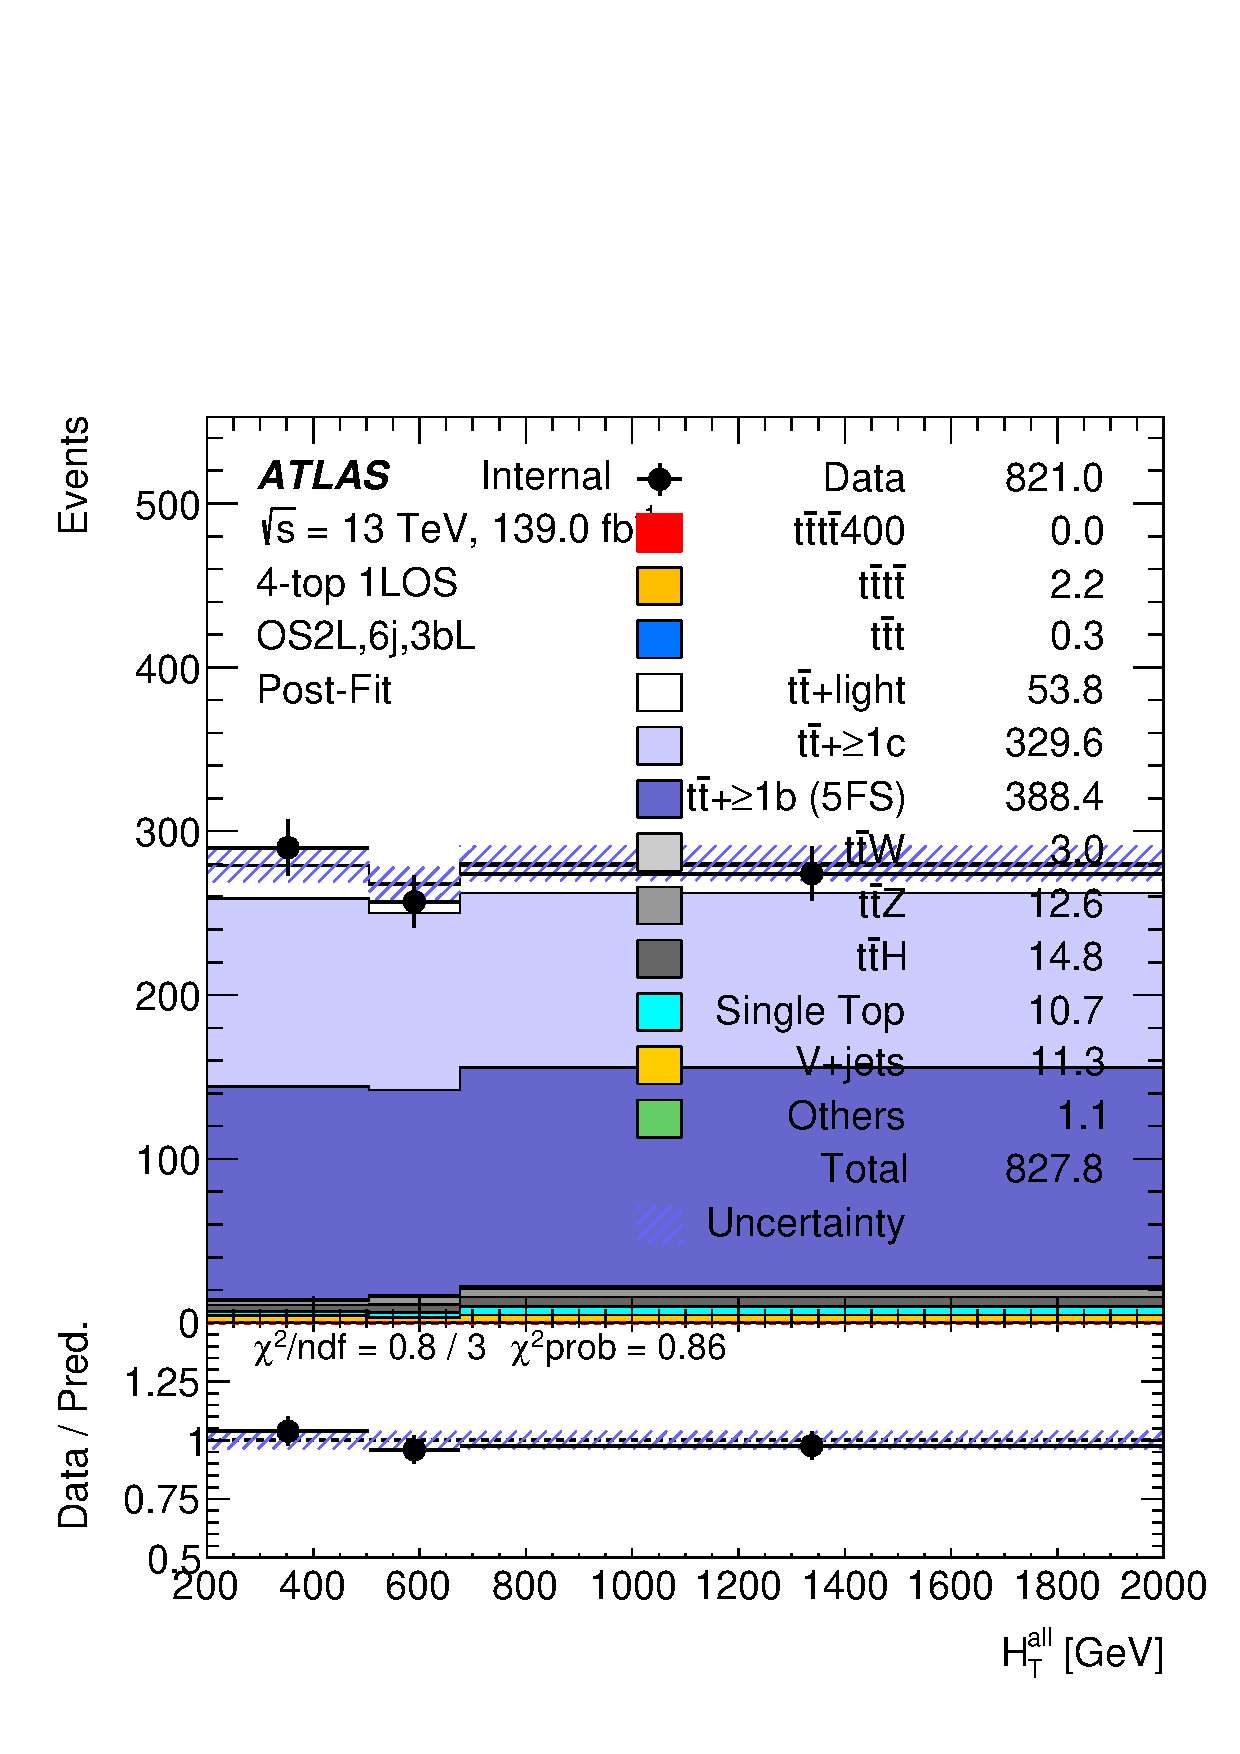
\includegraphics[width=0.31 \textwidth]{figures/fits/GNN/400/all/data/Plots/os2l_6j3bL_postFit.pdf} &
        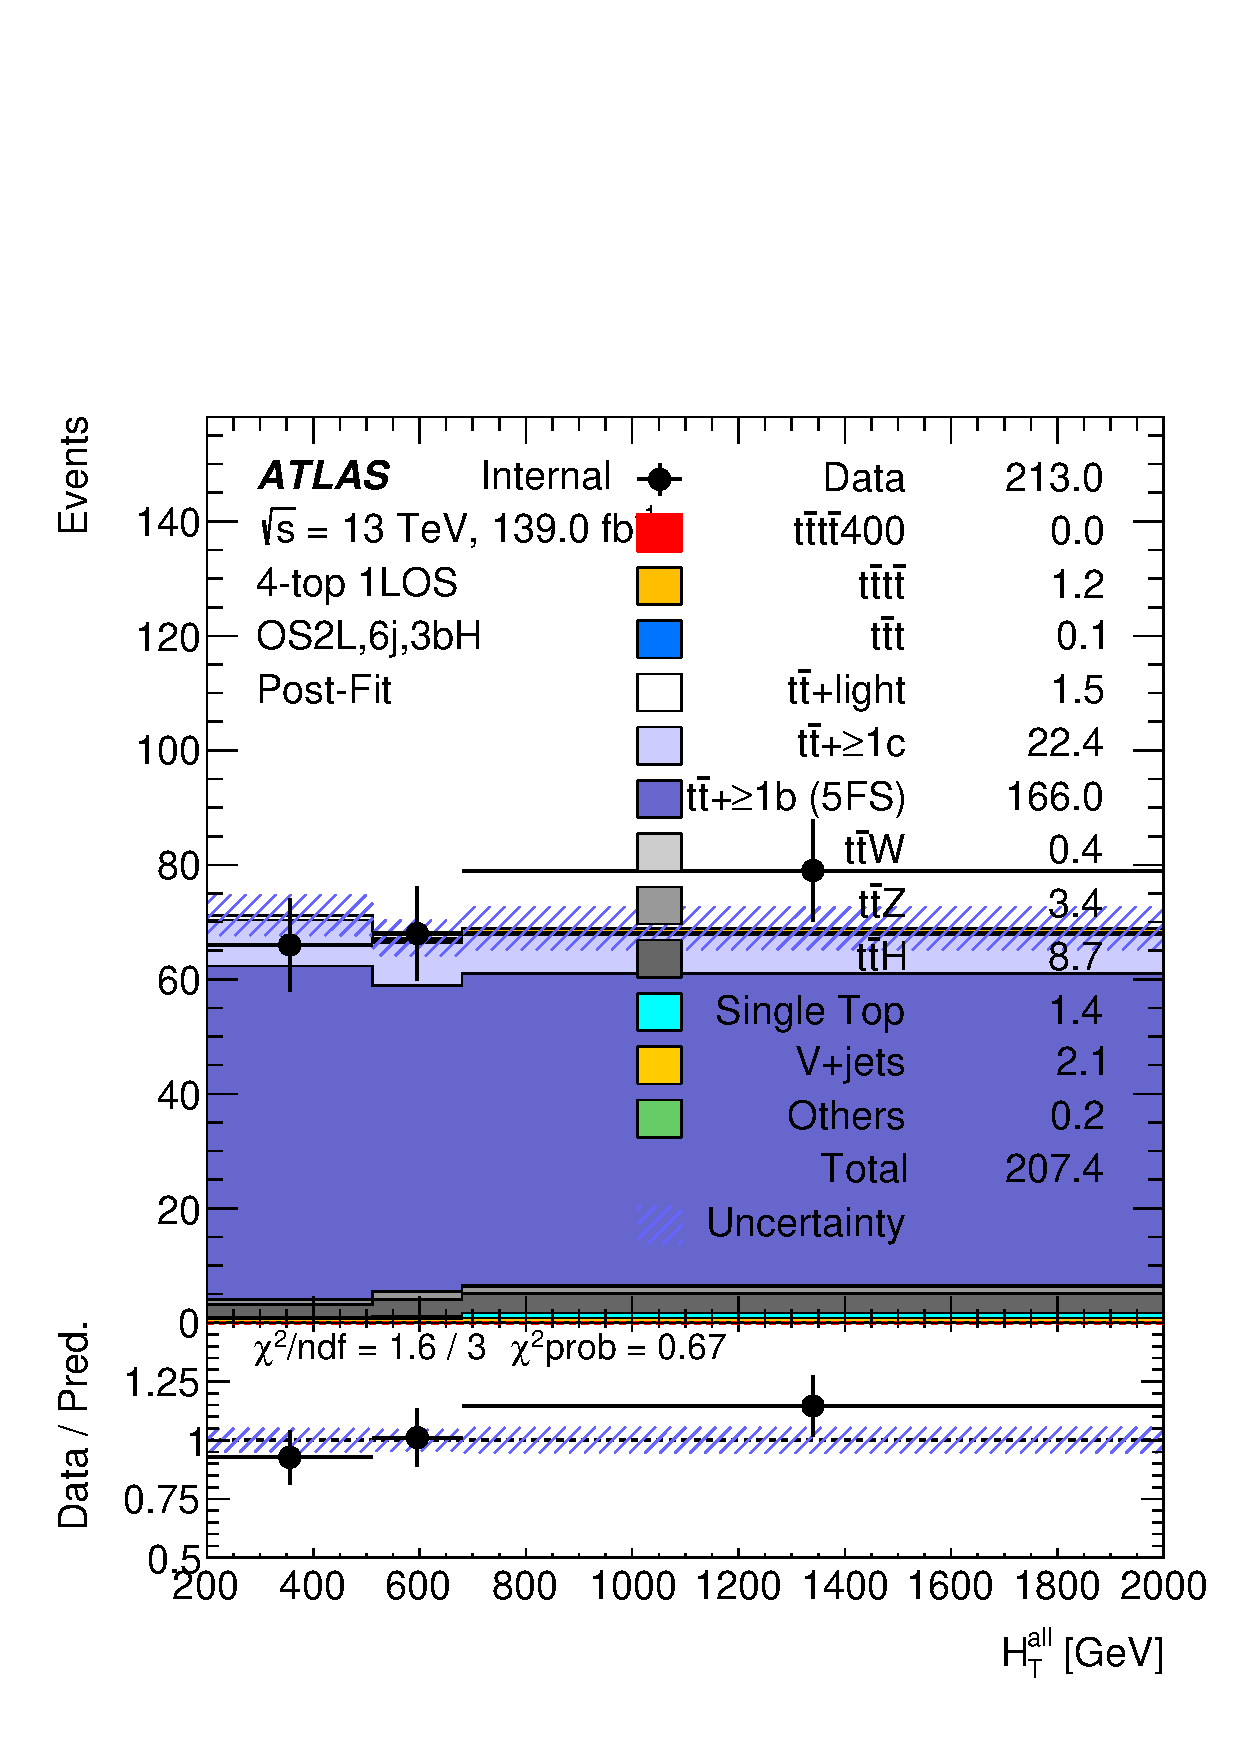
\includegraphics[width=0.31 \textwidth]{figures/fits/GNN/400/all/data/Plots/os2l_6j3bH_postFit.pdf} &
        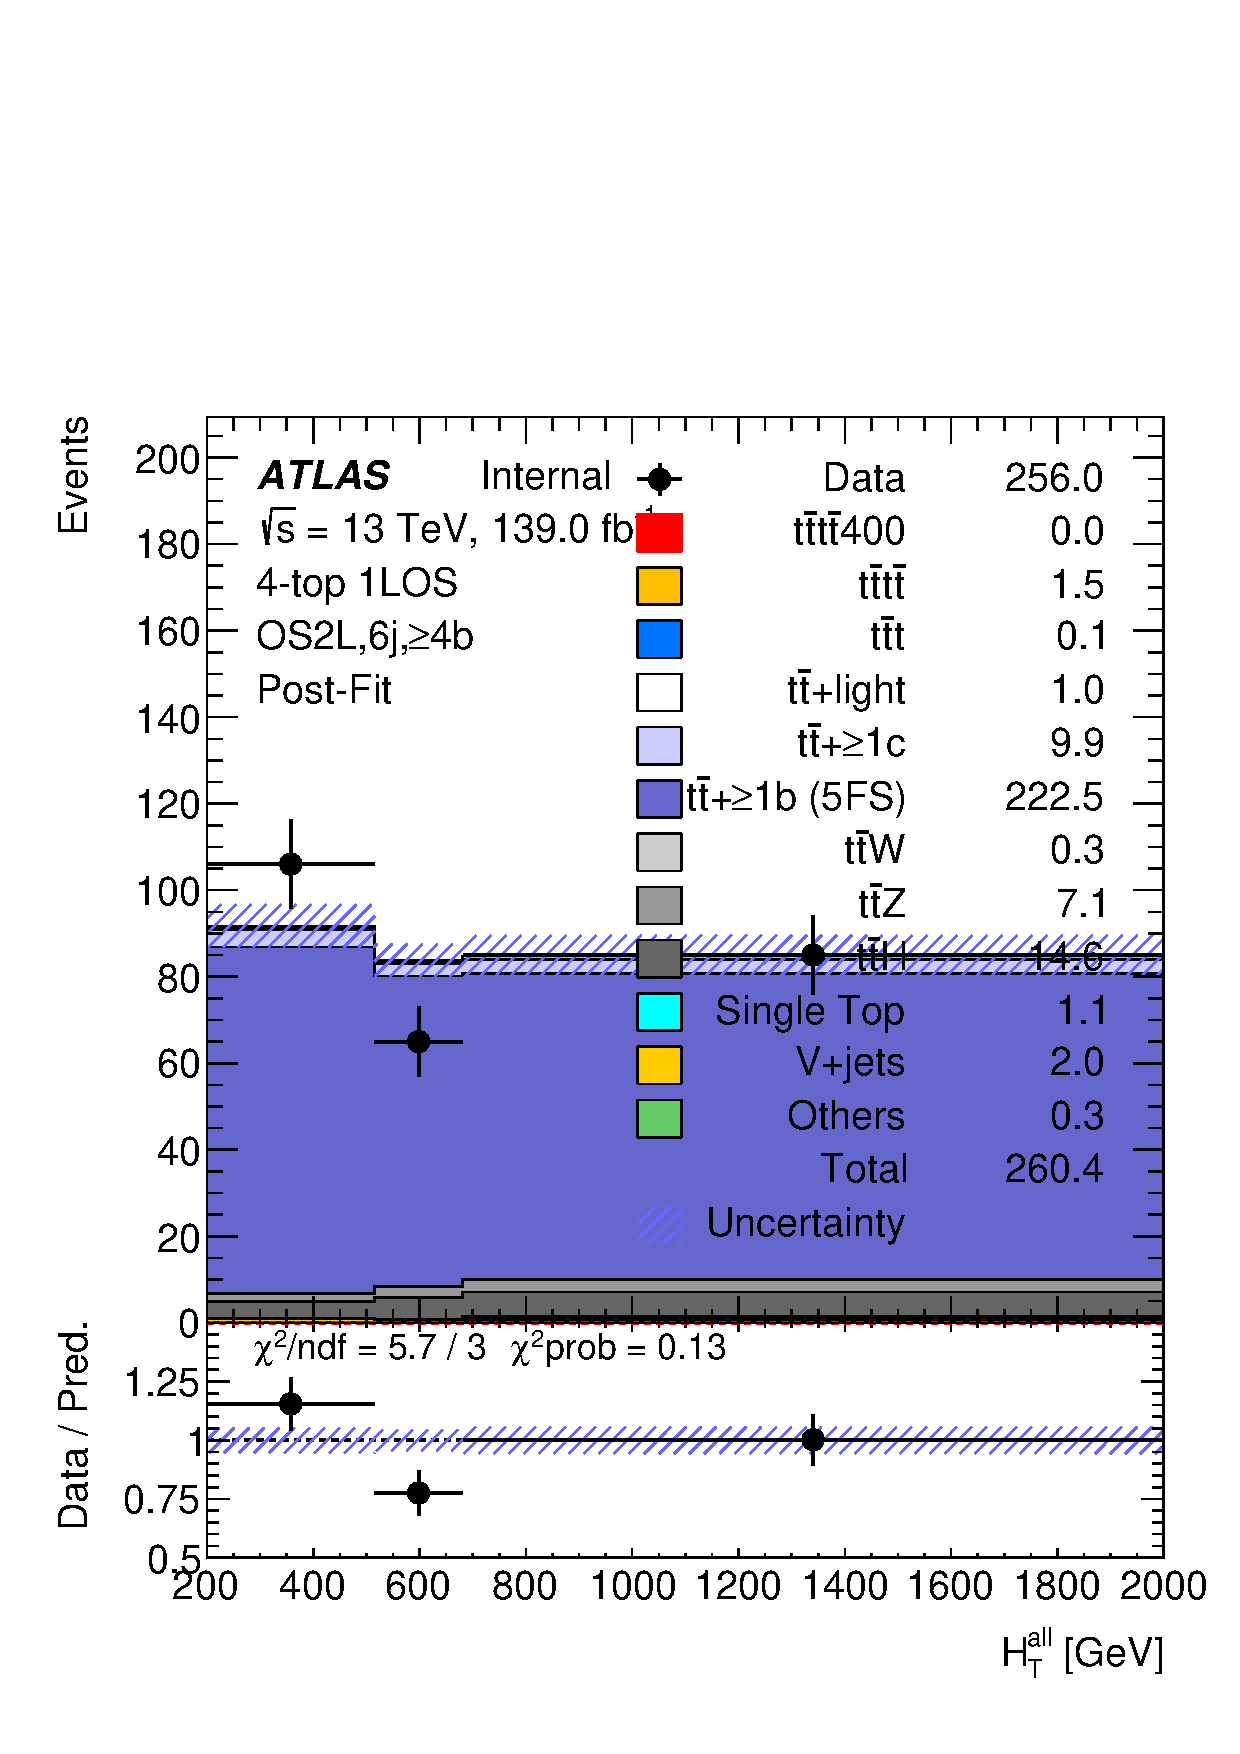
\includegraphics[width=0.31 \textwidth]{figures/fits/GNN/400/all/data/Plots/os2l_6jge4b_postFit.pdf} \\

        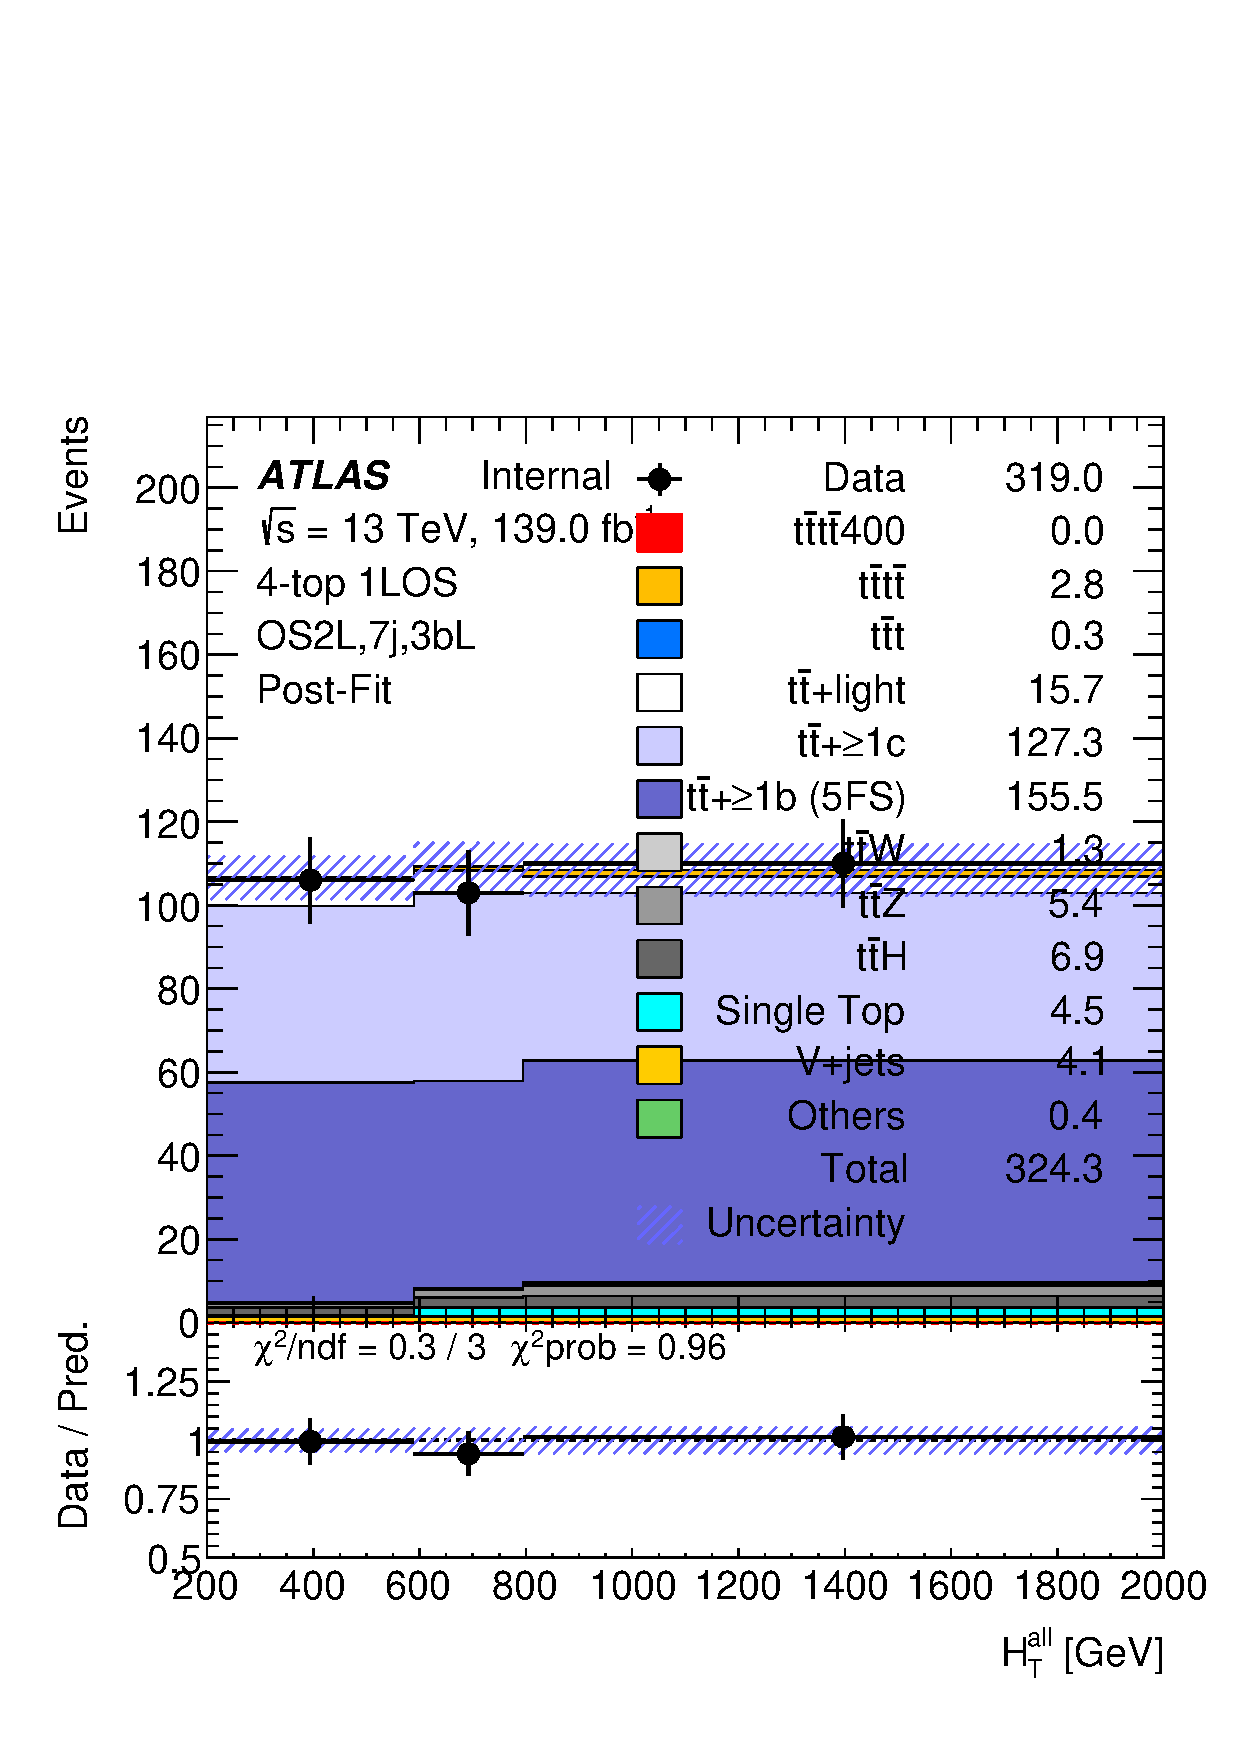
\includegraphics[width=0.31 \textwidth]{figures/fits/GNN/400/all/data/Plots/os2l_7j3bL_postFit.pdf} &
        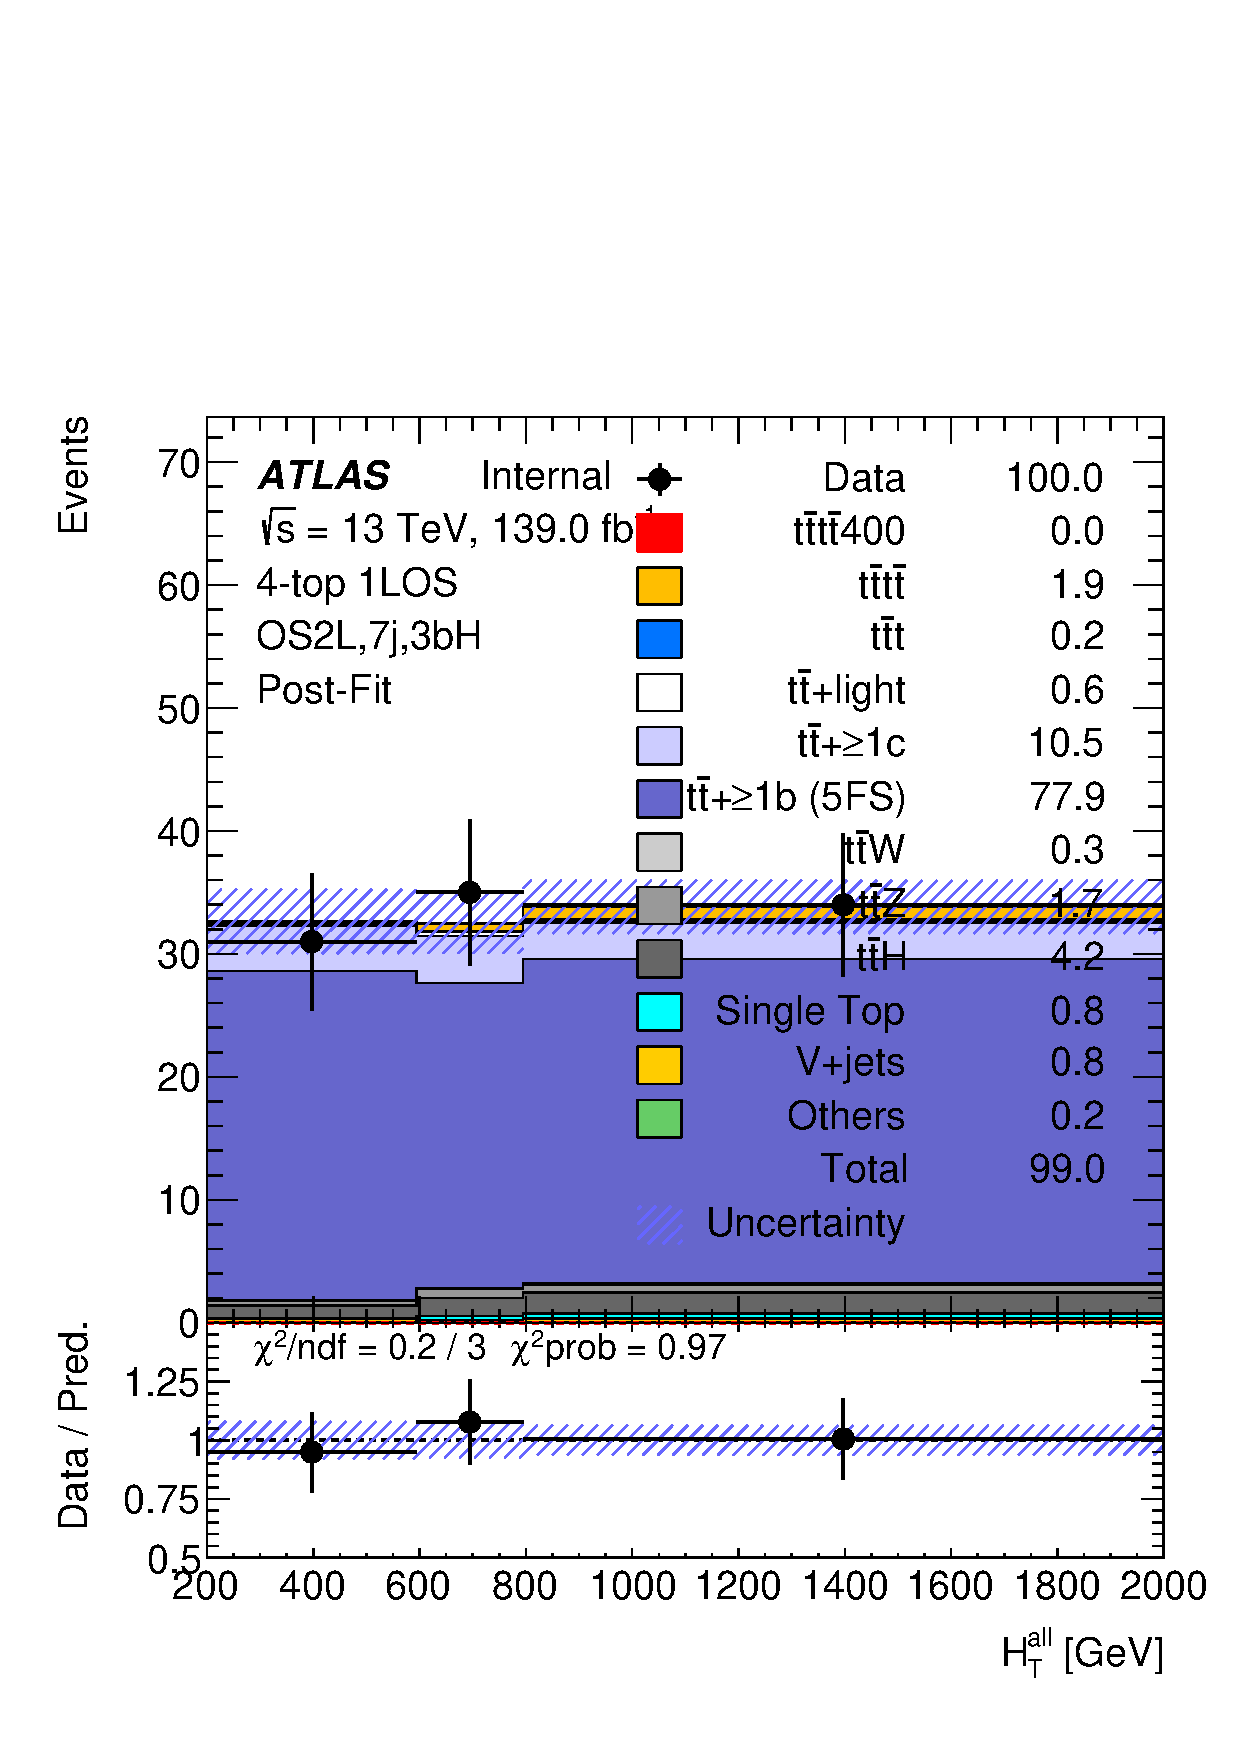
\includegraphics[width=0.31 \textwidth]{figures/fits/GNN/400/all/data/Plots/os2l_7j3bH_postFit.pdf} &
        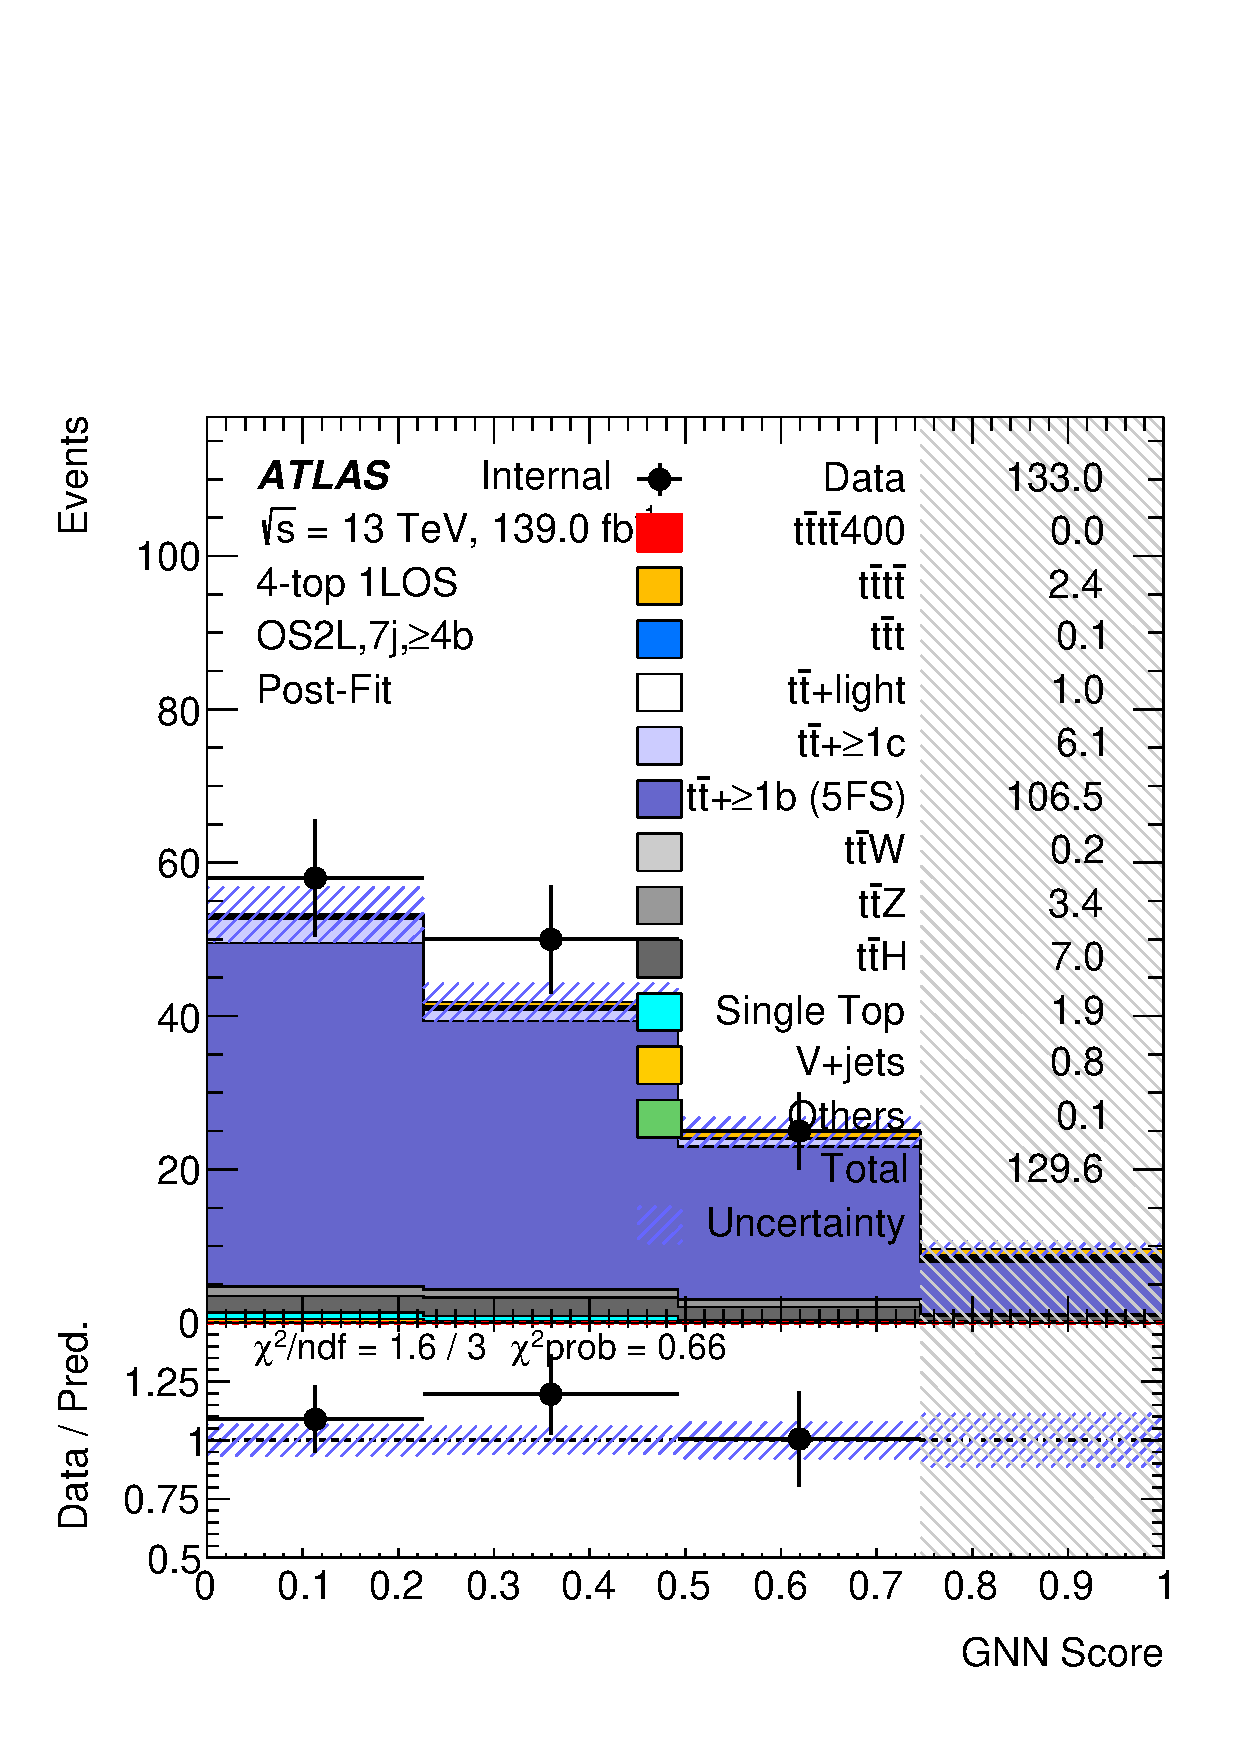
\includegraphics[width=0.31 \textwidth]{figures/fits/GNN/400/all/data/Plots/os2l_7jge4b_postFit.pdf} \\

        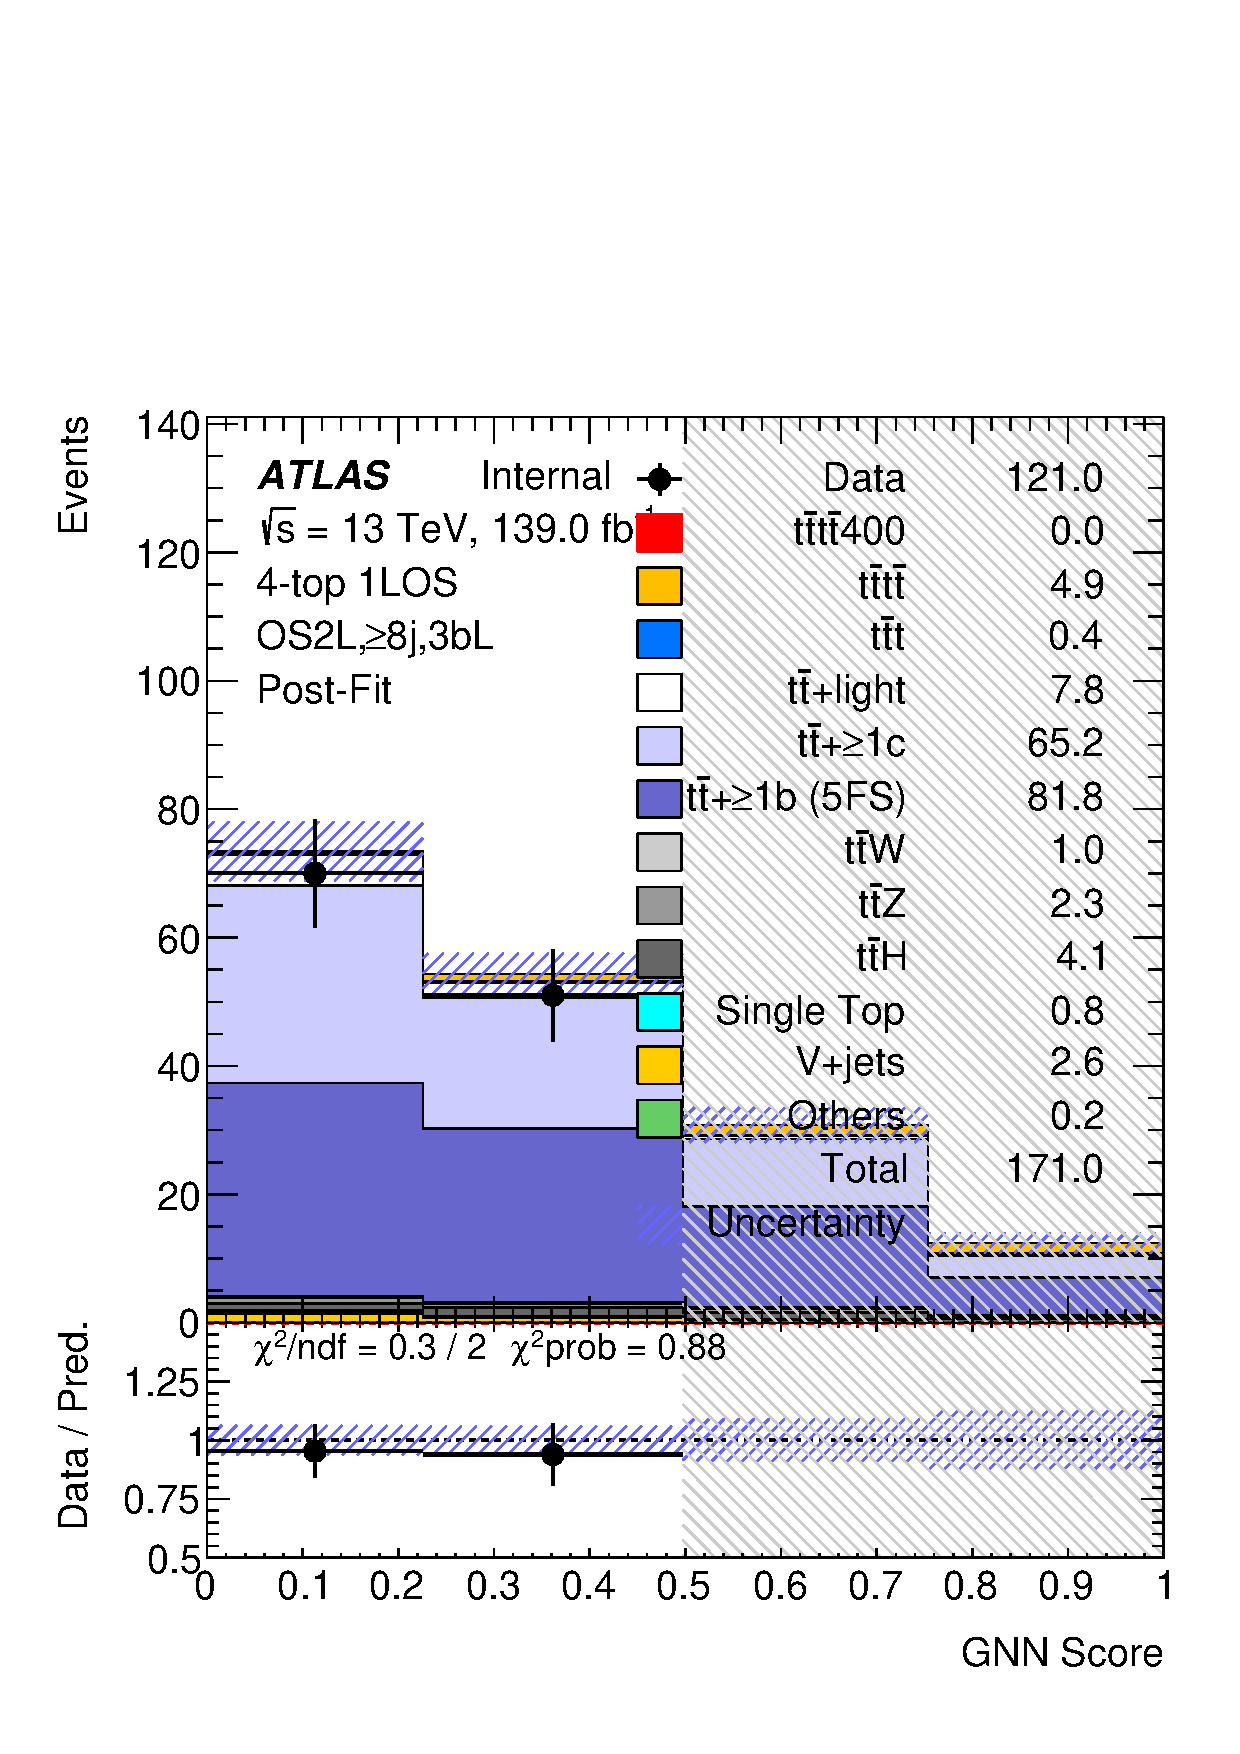
\includegraphics[width=0.31 \textwidth]{figures/fits/GNN/400/all/data/Plots/os2l_ge8j3bL_postFit.pdf} &
        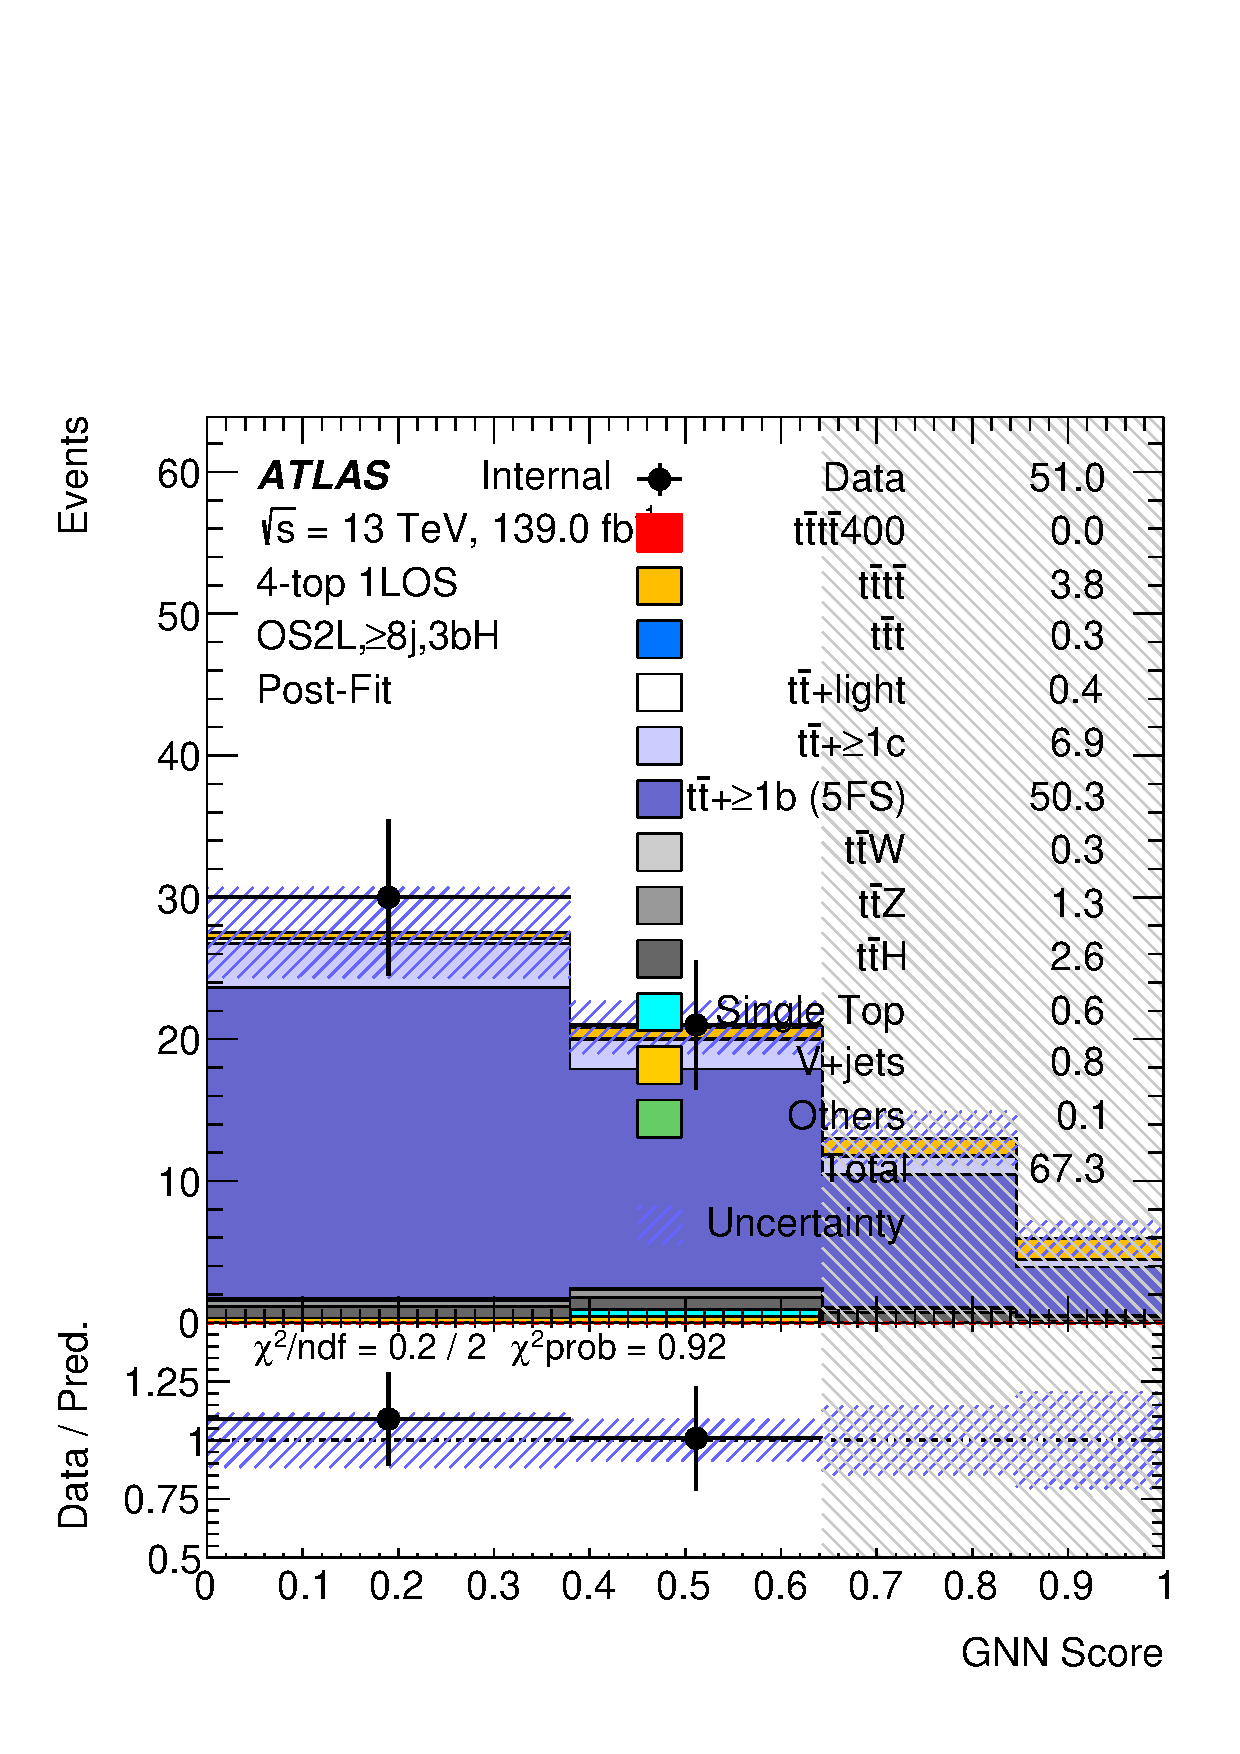
\includegraphics[width=0.31 \textwidth]{figures/fits/GNN/400/all/data/Plots/os2l_ge8j3bH_postFit.pdf} &
        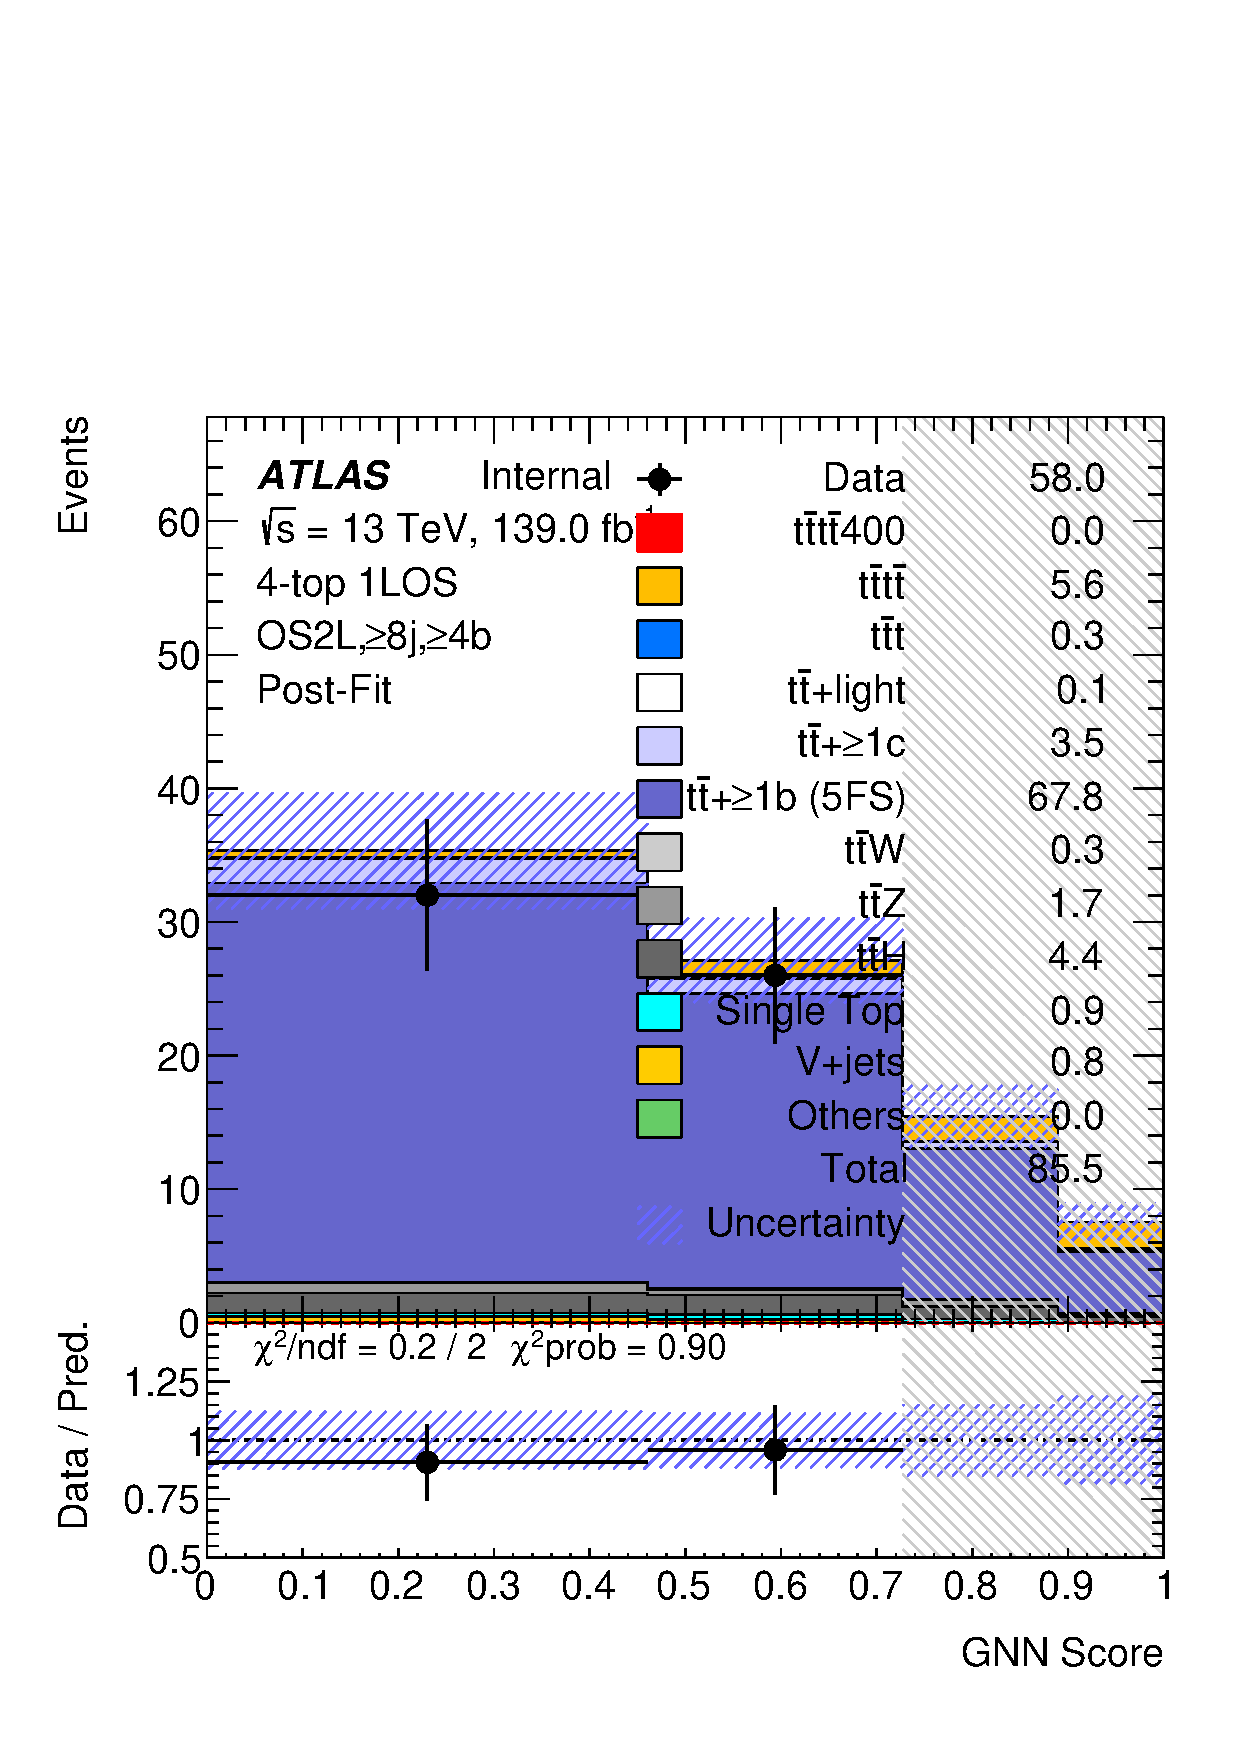
\includegraphics[width=0.31 \textwidth]{figures/fits/GNN/400/all/data/Plots/os2l_ge8jge4b_postFit.pdf} \\
        \end{tabular}
        \caption{\label{fig:Postfit_Yields_2L}Post-fit distributions for 2LOS regions associated with different signal and background samples, compared with data yields for mH = 400 GeV. The fit is done using all regions (1L+2L)}
\end{center}
\end{figure}


\begin{figure}[htbp!]
  \centering
  \begin{subfigure}[t]{0.32\textwidth}
    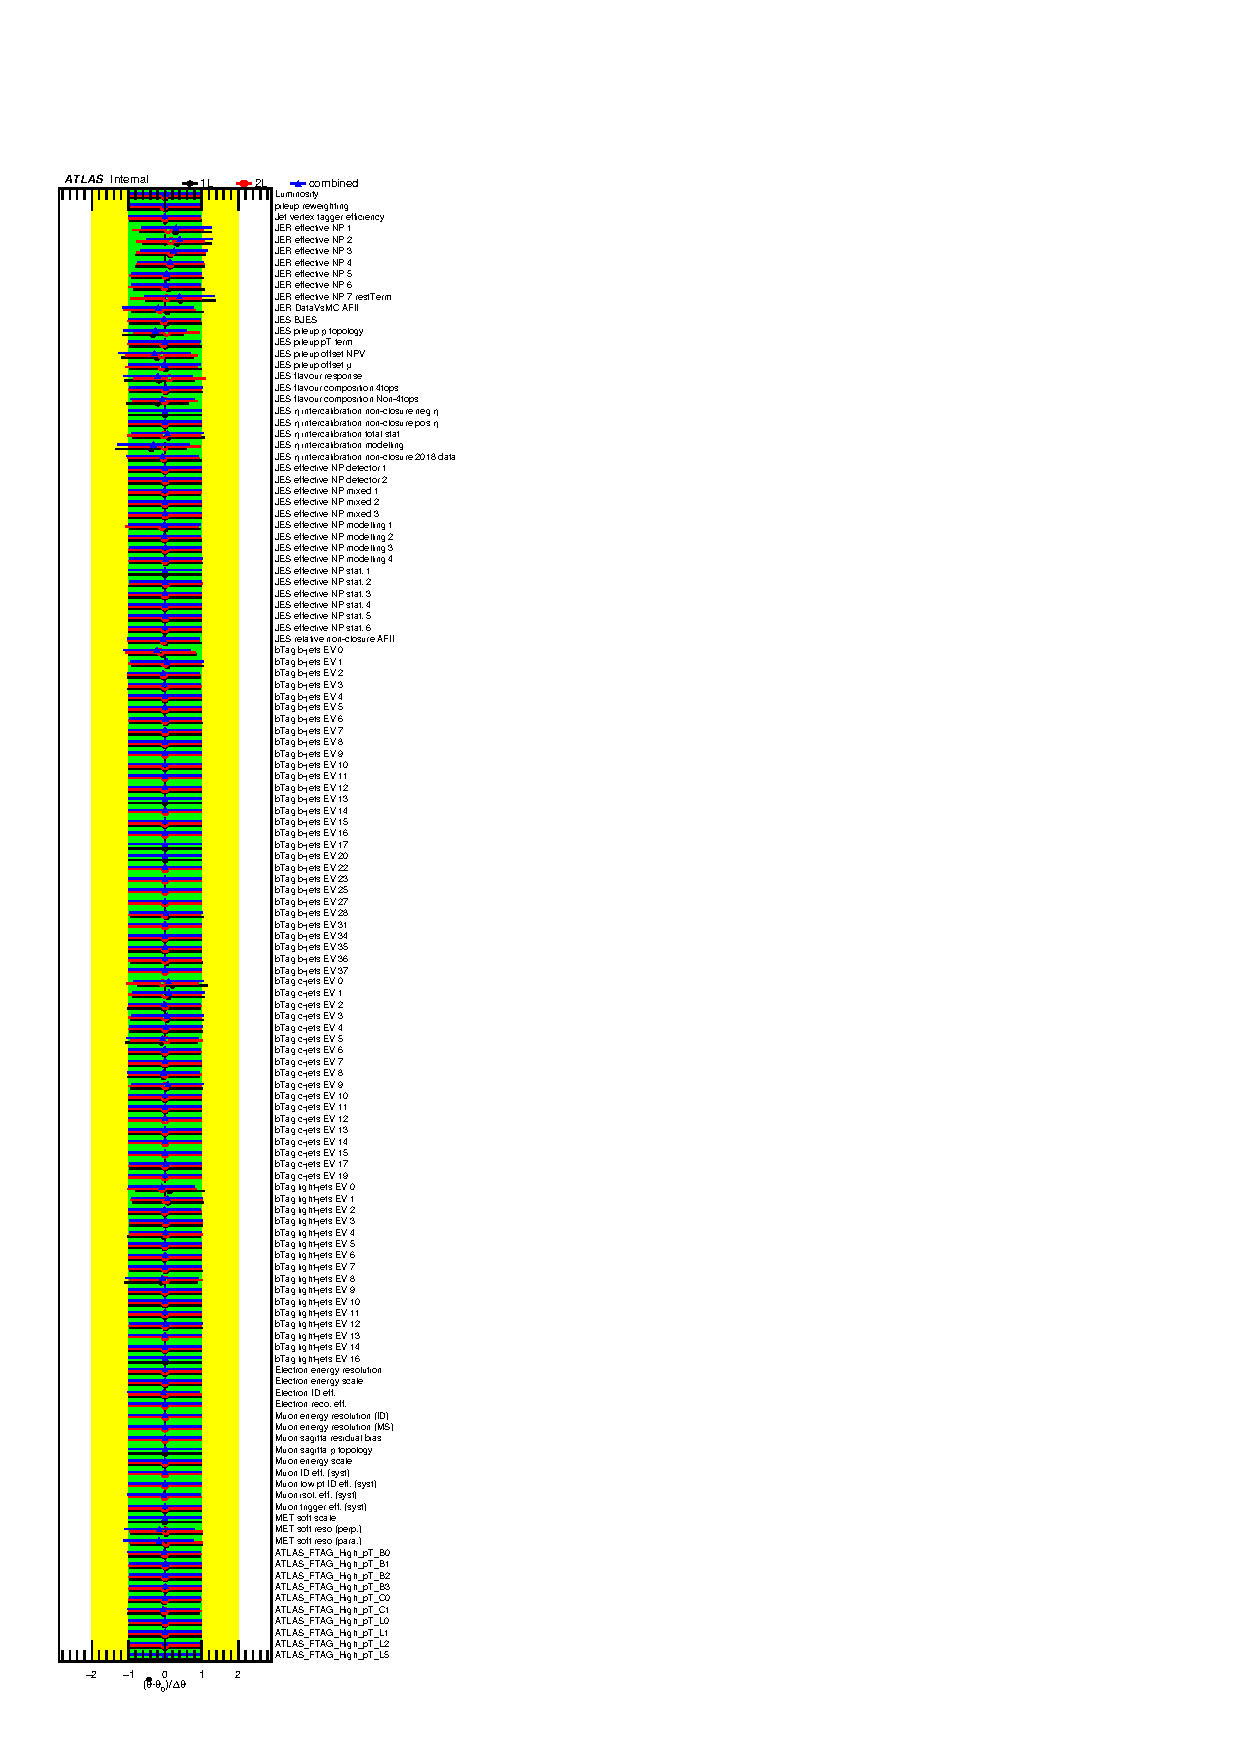
\includegraphics[width=\linewidth]{figures/fits/comparisons/selections/GNN/400/data/NuisPar_comp_Instrumental.pdf}
    \subcaption{mH=400\gev}
    \label{fig:data_NP_mH400}
  \end{subfigure}
  \begin{subfigure}[t]{0.32\textwidth}
    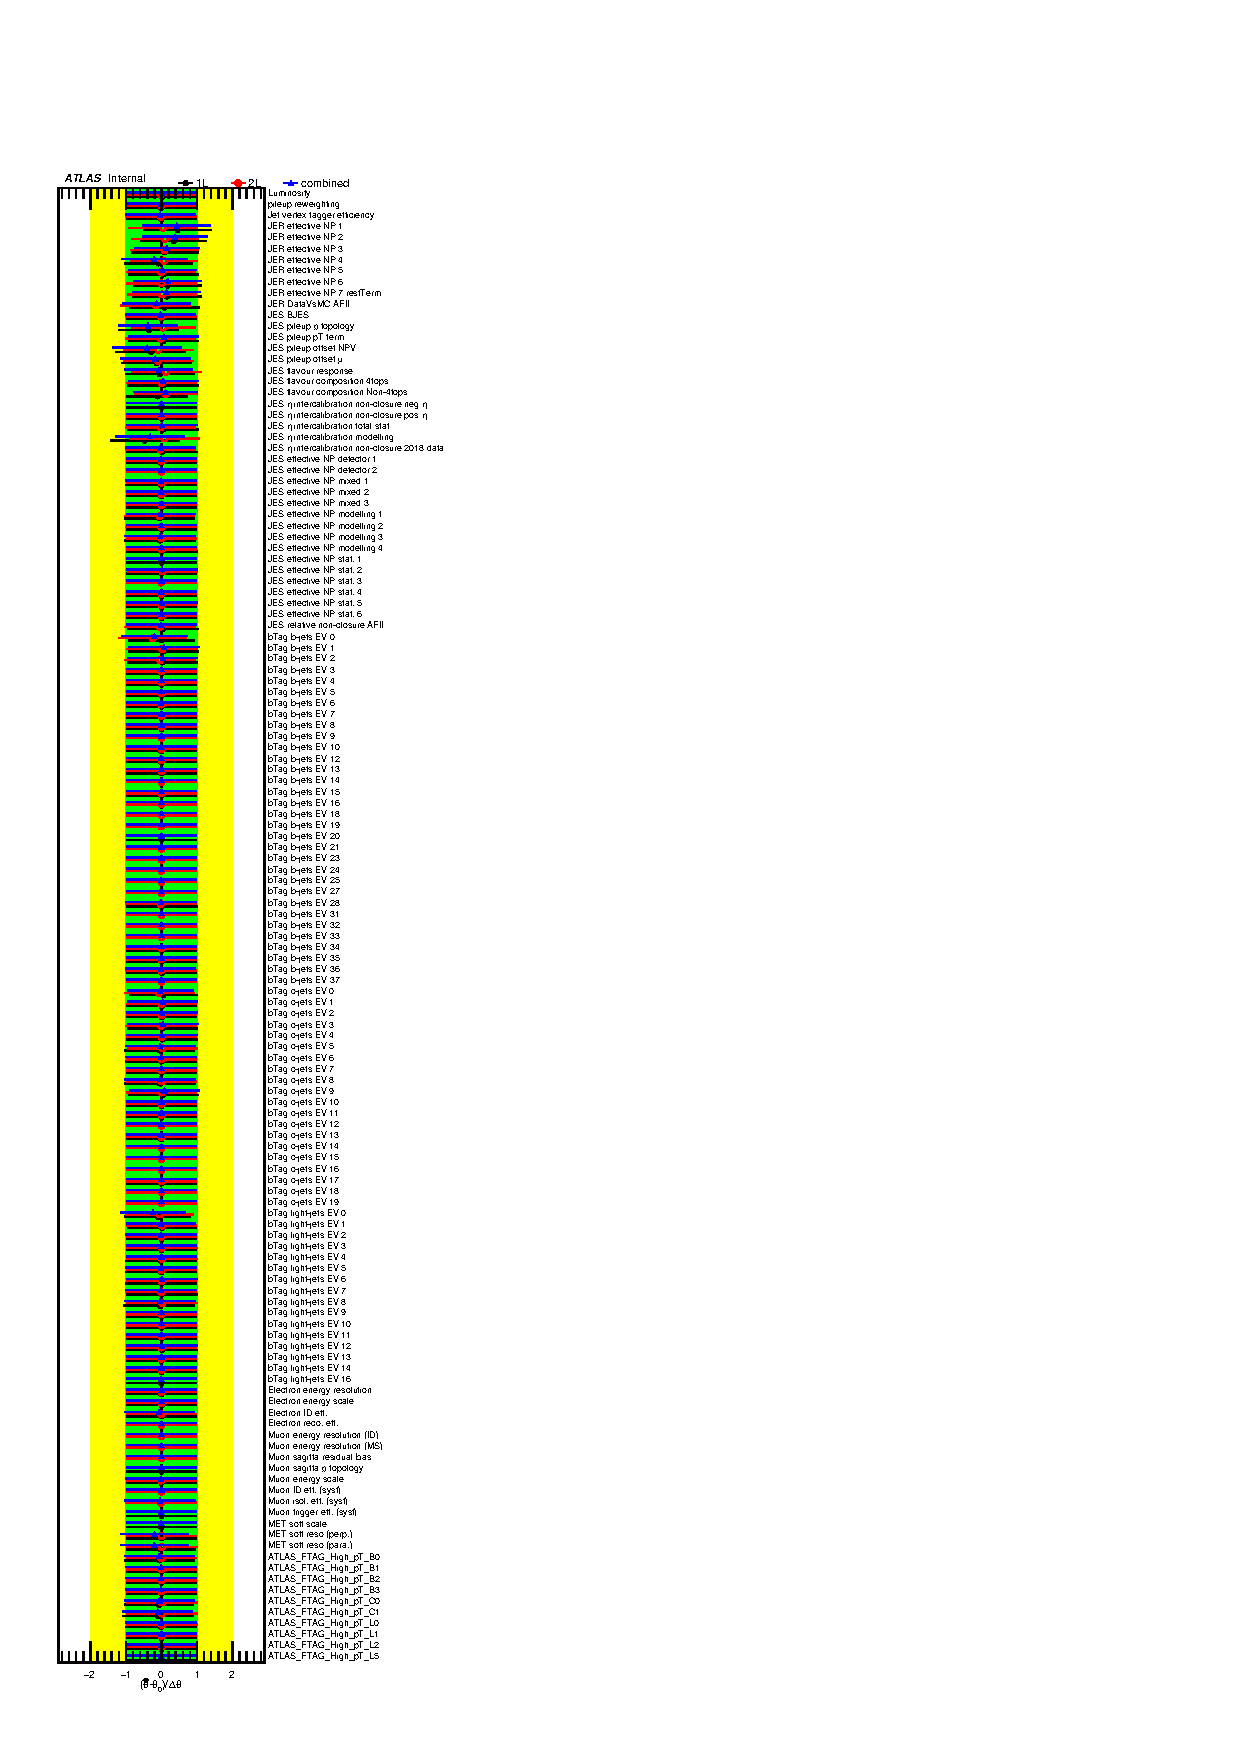
\includegraphics[width=\linewidth]{figures/fits/comparisons/selections/GNN/700/data/NuisPar_comp_Instrumental.pdf}
    \subcaption{mH=700\gev}
    \label{fig:data_NP_mH400}
  \end{subfigure}
  \begin{subfigure}[t]{0.32\textwidth}
    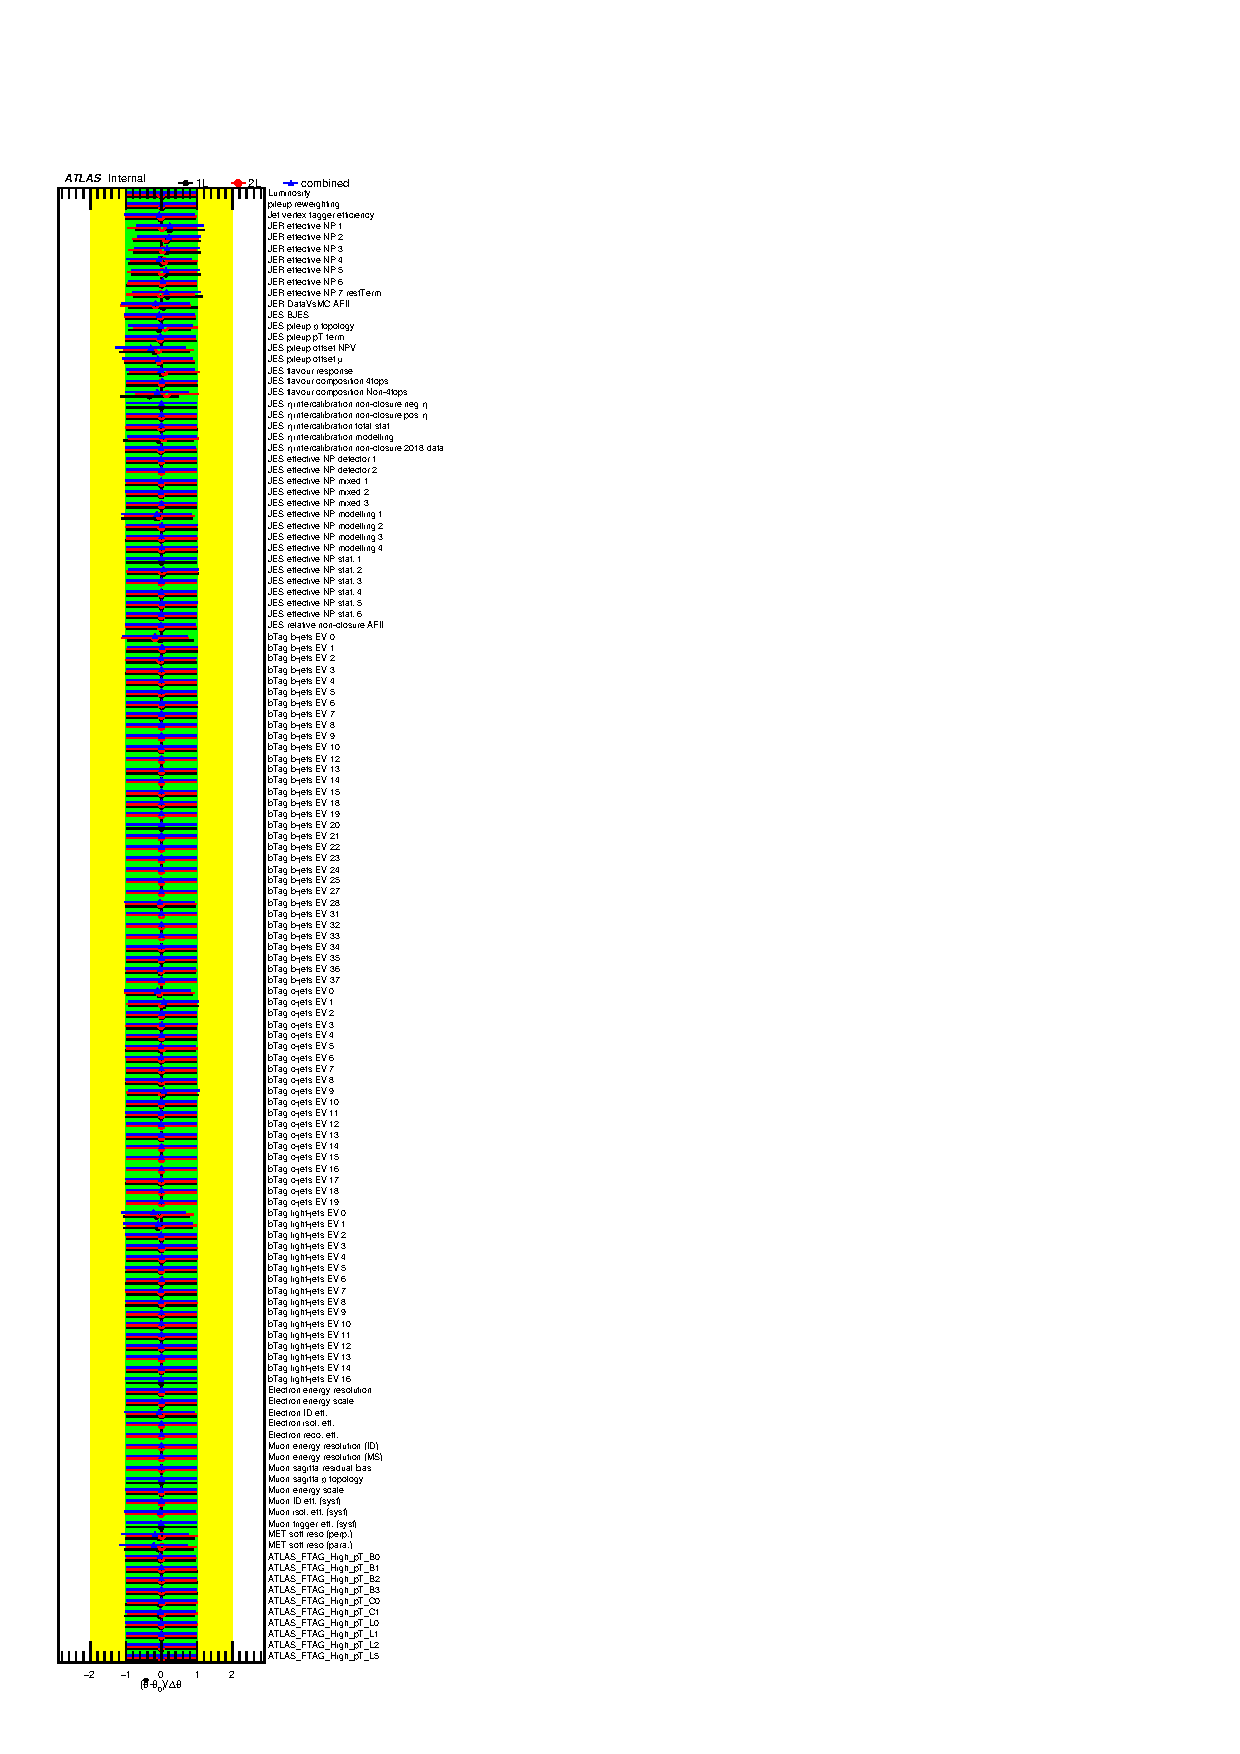
\includegraphics[width=\linewidth]{figures/fits/comparisons/selections/GNN/1000/data/NuisPar_comp_Instrumental.pdf}
    \subcaption{mH=1000\gev}
    \label{fig:data_NP_mH400}
  \end{subfigure}
  \caption{\label{fig:data_NP_instrumental}Fitted pulls and constraints for the nuisance parameters corresponding to the instrumental systematic uncertainties for the blinded Data fit for three mass points. Comparison is done for three fits: using only 1L regions, using only 2LOS regions and using all regions.}
\end{figure}


\begin{figure}[htbp!]
  \centering
  \begin{subfigure}[t]{0.32\textwidth}
    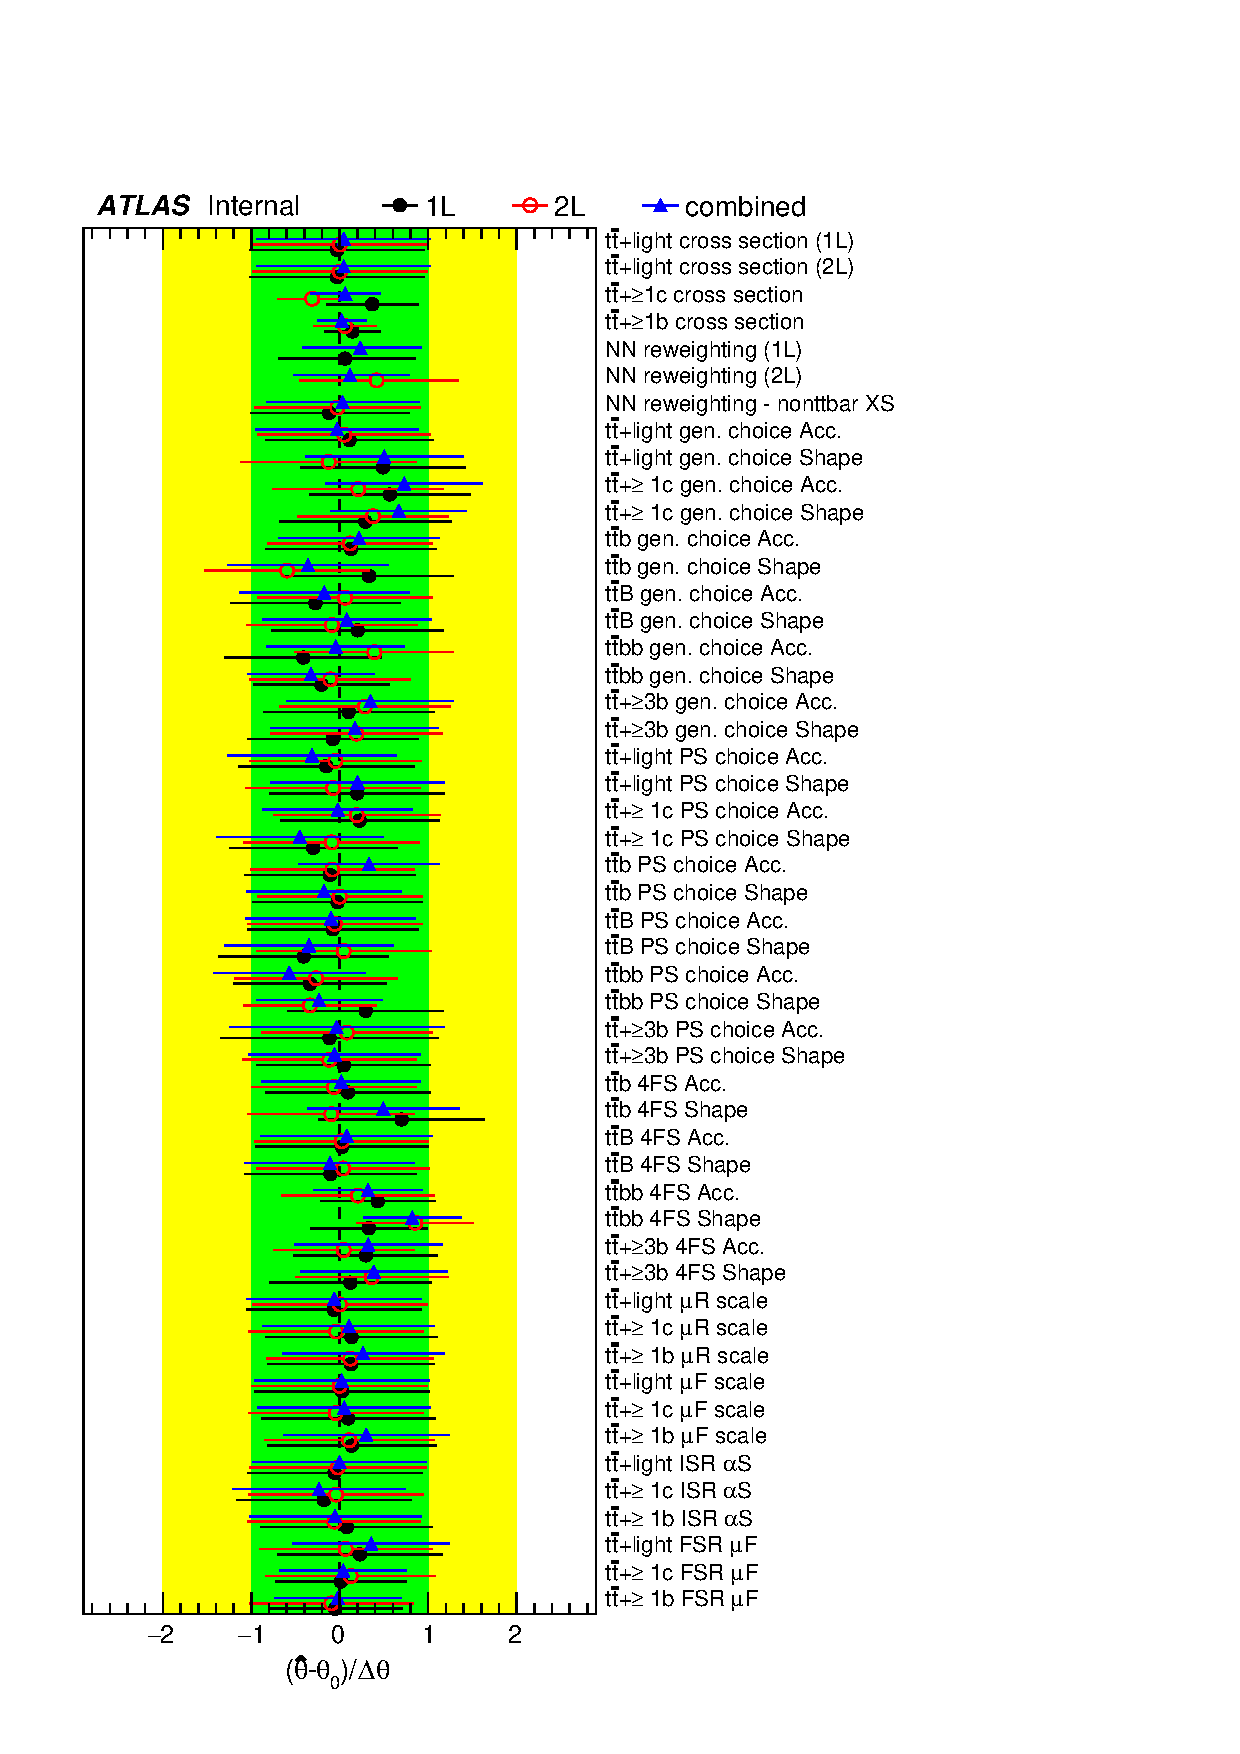
\includegraphics[width=\linewidth]{figures/fits/comparisons/selections/GNN/400/data/NuisPar_comp_ttbar.pdf}
    \subcaption{mH=400\gev}
    \label{fig:data_NP_mH400}
  \end{subfigure}
  \begin{subfigure}[t]{0.32\textwidth}
    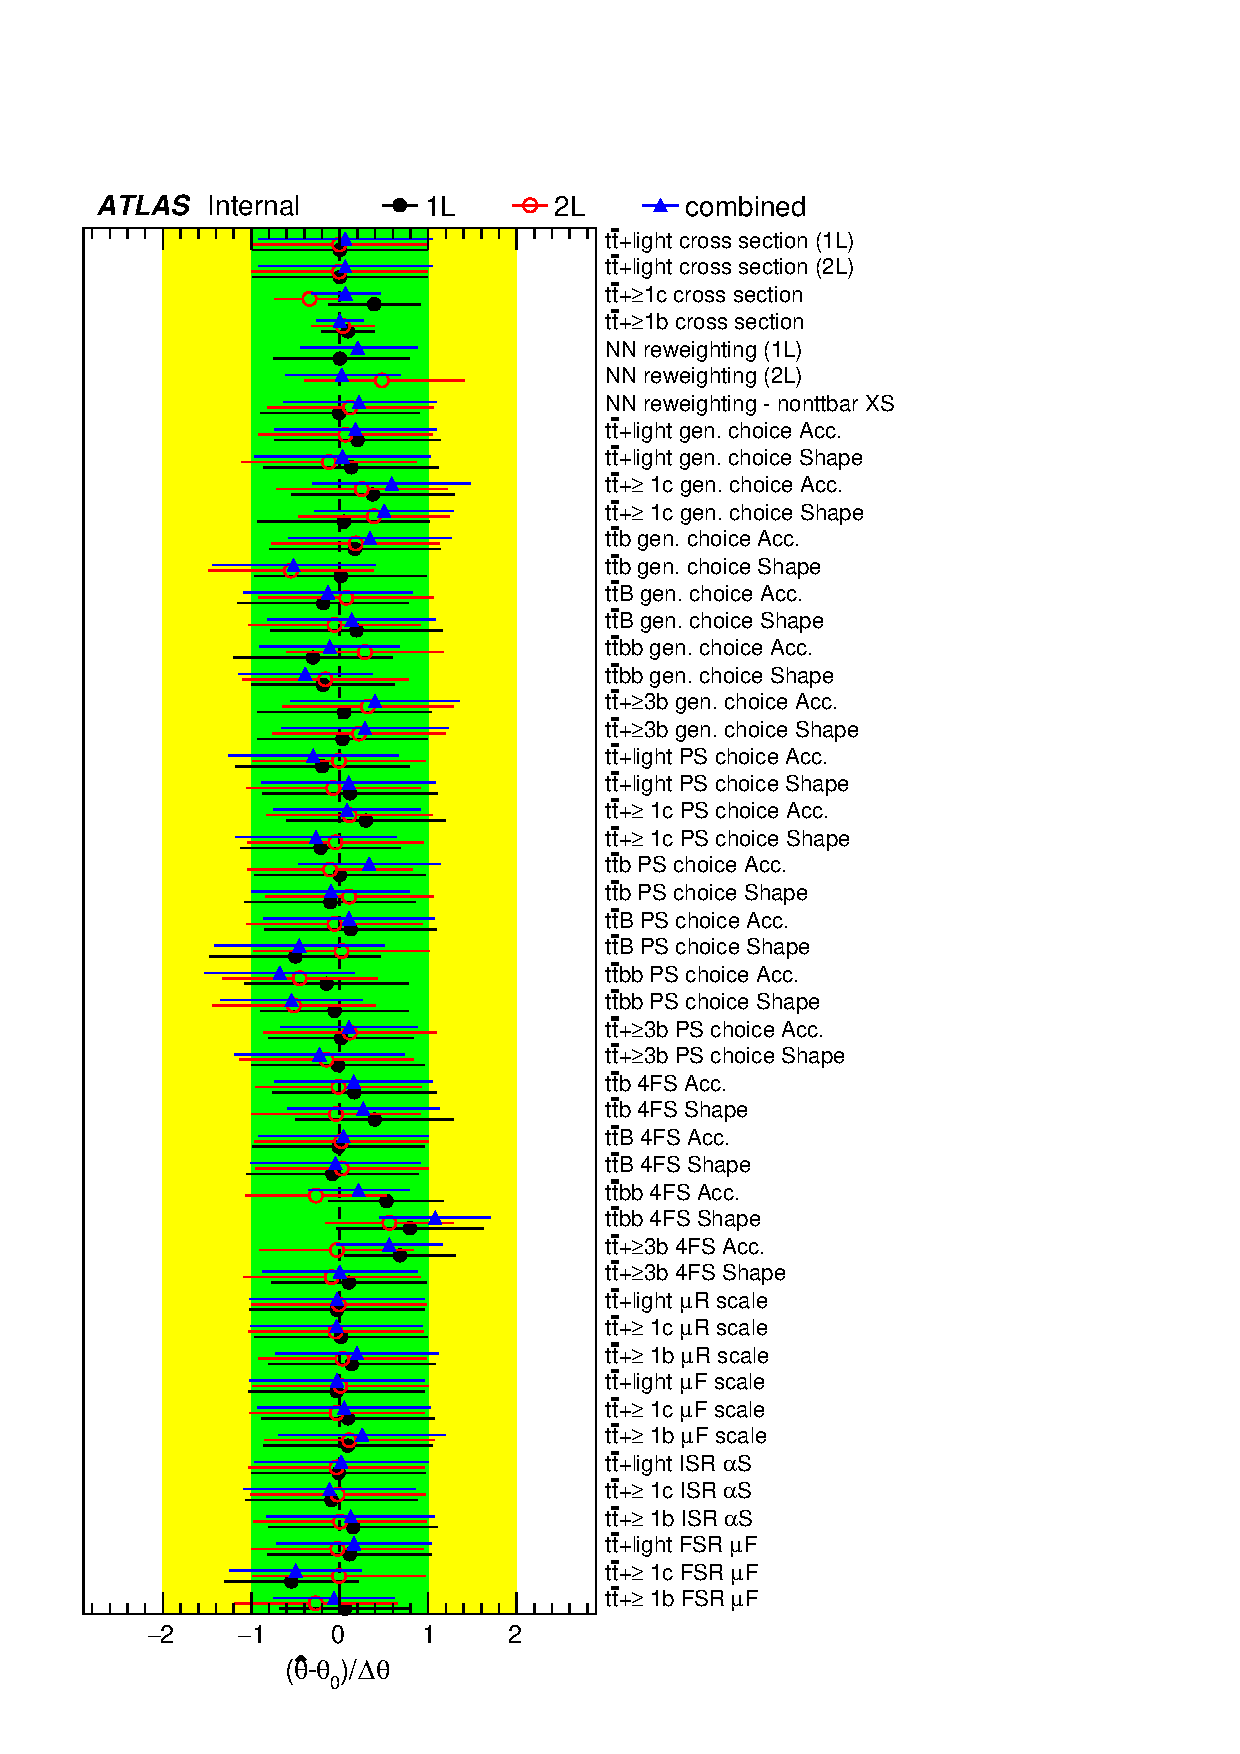
\includegraphics[width=\linewidth]{figures/fits/comparisons/selections/GNN/700/data/NuisPar_comp_ttbar.pdf}
    \subcaption{mH=700\gev}
    \label{fig:data_NP_mH400}
  \end{subfigure}
  \begin{subfigure}[t]{0.32\textwidth}
    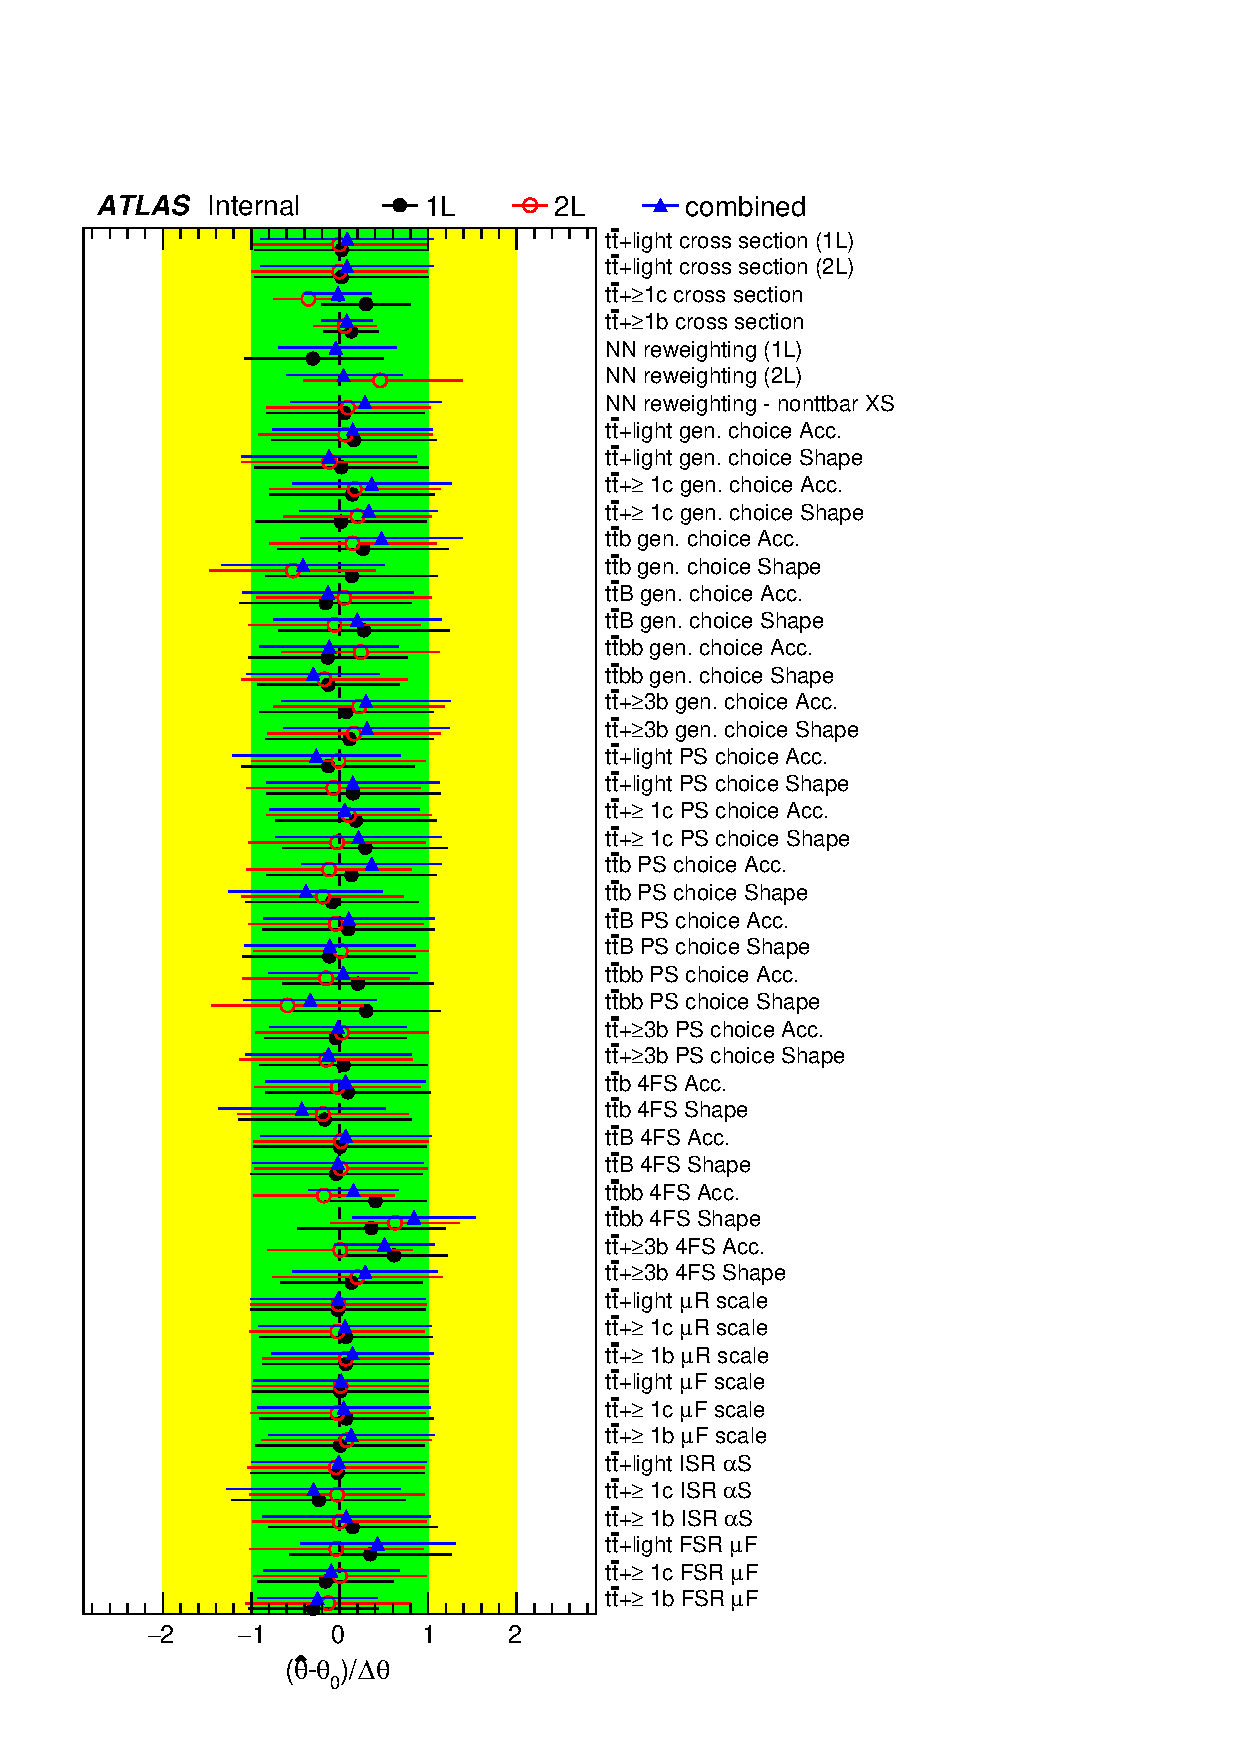
\includegraphics[width=\linewidth]{figures/fits/comparisons/selections/GNN/1000/data/NuisPar_comp_ttbar.pdf}
    \subcaption{mH=1000\gev}
    \label{fig:data_NP_mH400}
  \end{subfigure}
  \caption{\label{fig:data_NP_ttbar}Fitted pulls and constraints for the nuisance parameters corresponding to the \ttbar systematic uncertainties for the blinded Data fit for three mass points. Comparison is done for three fits: using only 1L regions, using only 2LOS regions and using all regions.}
\end{figure}


\begin{figure}[htbp!]
  \centering
  \begin{subfigure}[t]{0.32\textwidth}
    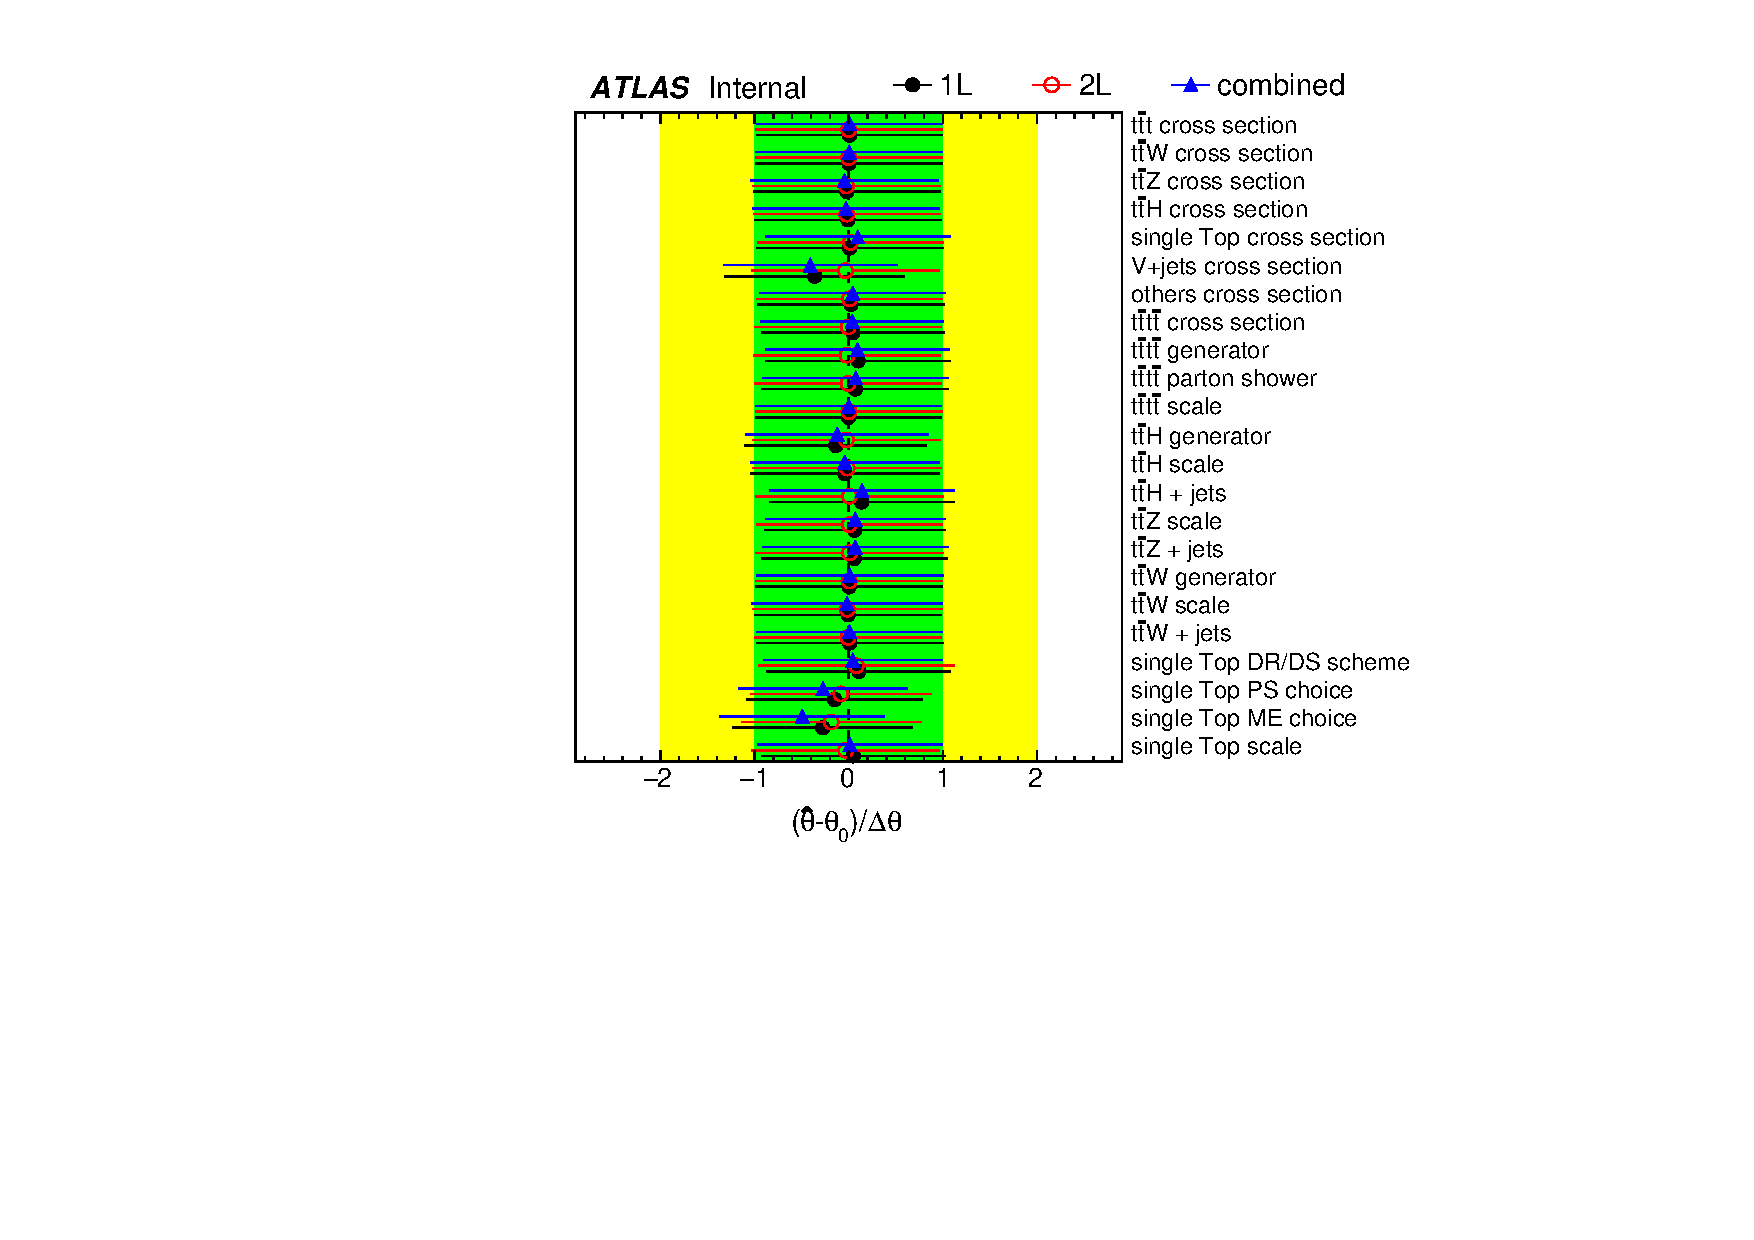
\includegraphics[width=\linewidth]{figures/fits/comparisons/selections/GNN/400/data/NuisPar_comp_Other.pdf}
    \subcaption{mH=400\gev}
    \label{fig:data_NP_mH400}
  \end{subfigure}
  \begin{subfigure}[t]{0.32\textwidth}
    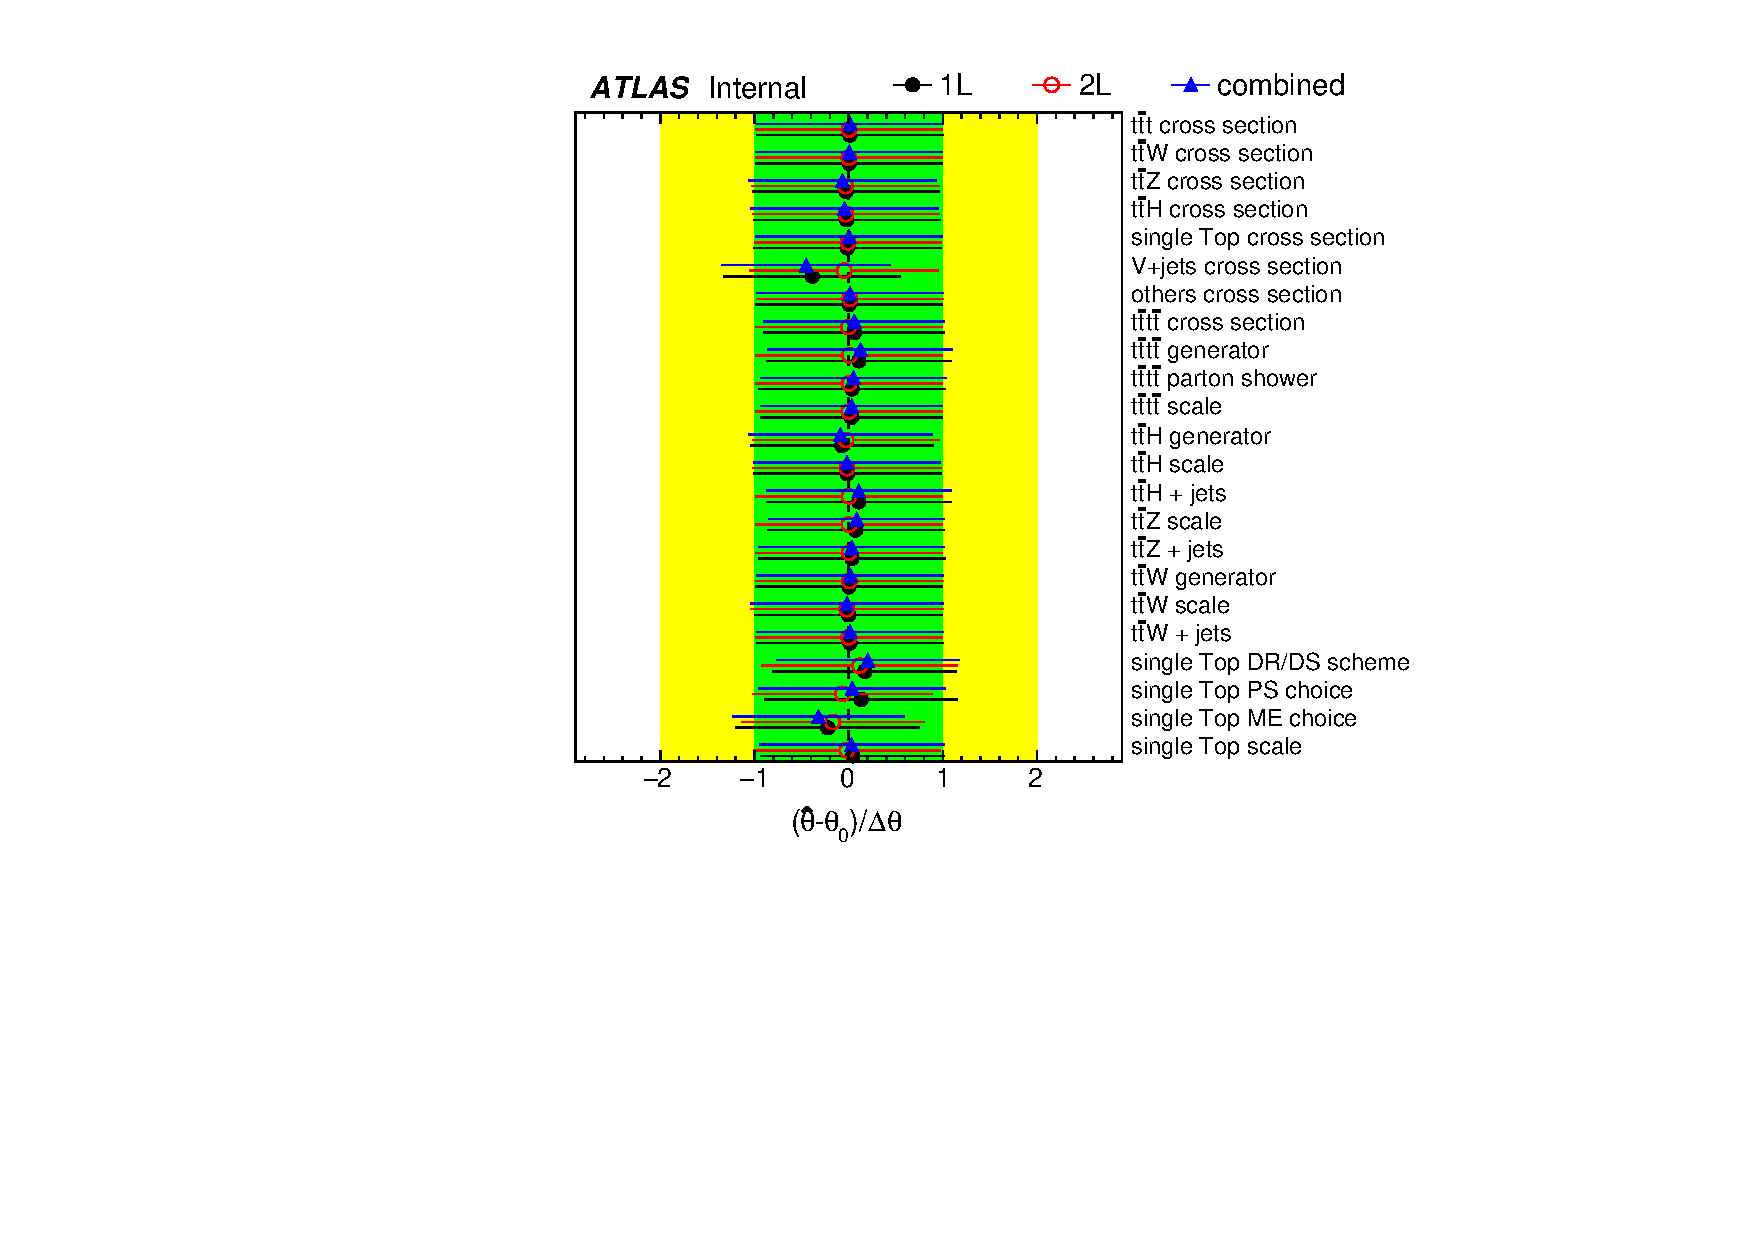
\includegraphics[width=\linewidth]{figures/fits/comparisons/selections/GNN/700/data/NuisPar_comp_Other.pdf}
    \subcaption{mH=700\gev}
    \label{fig:data_NP_mH400}
  \end{subfigure}
  \begin{subfigure}[t]{0.32\textwidth}
    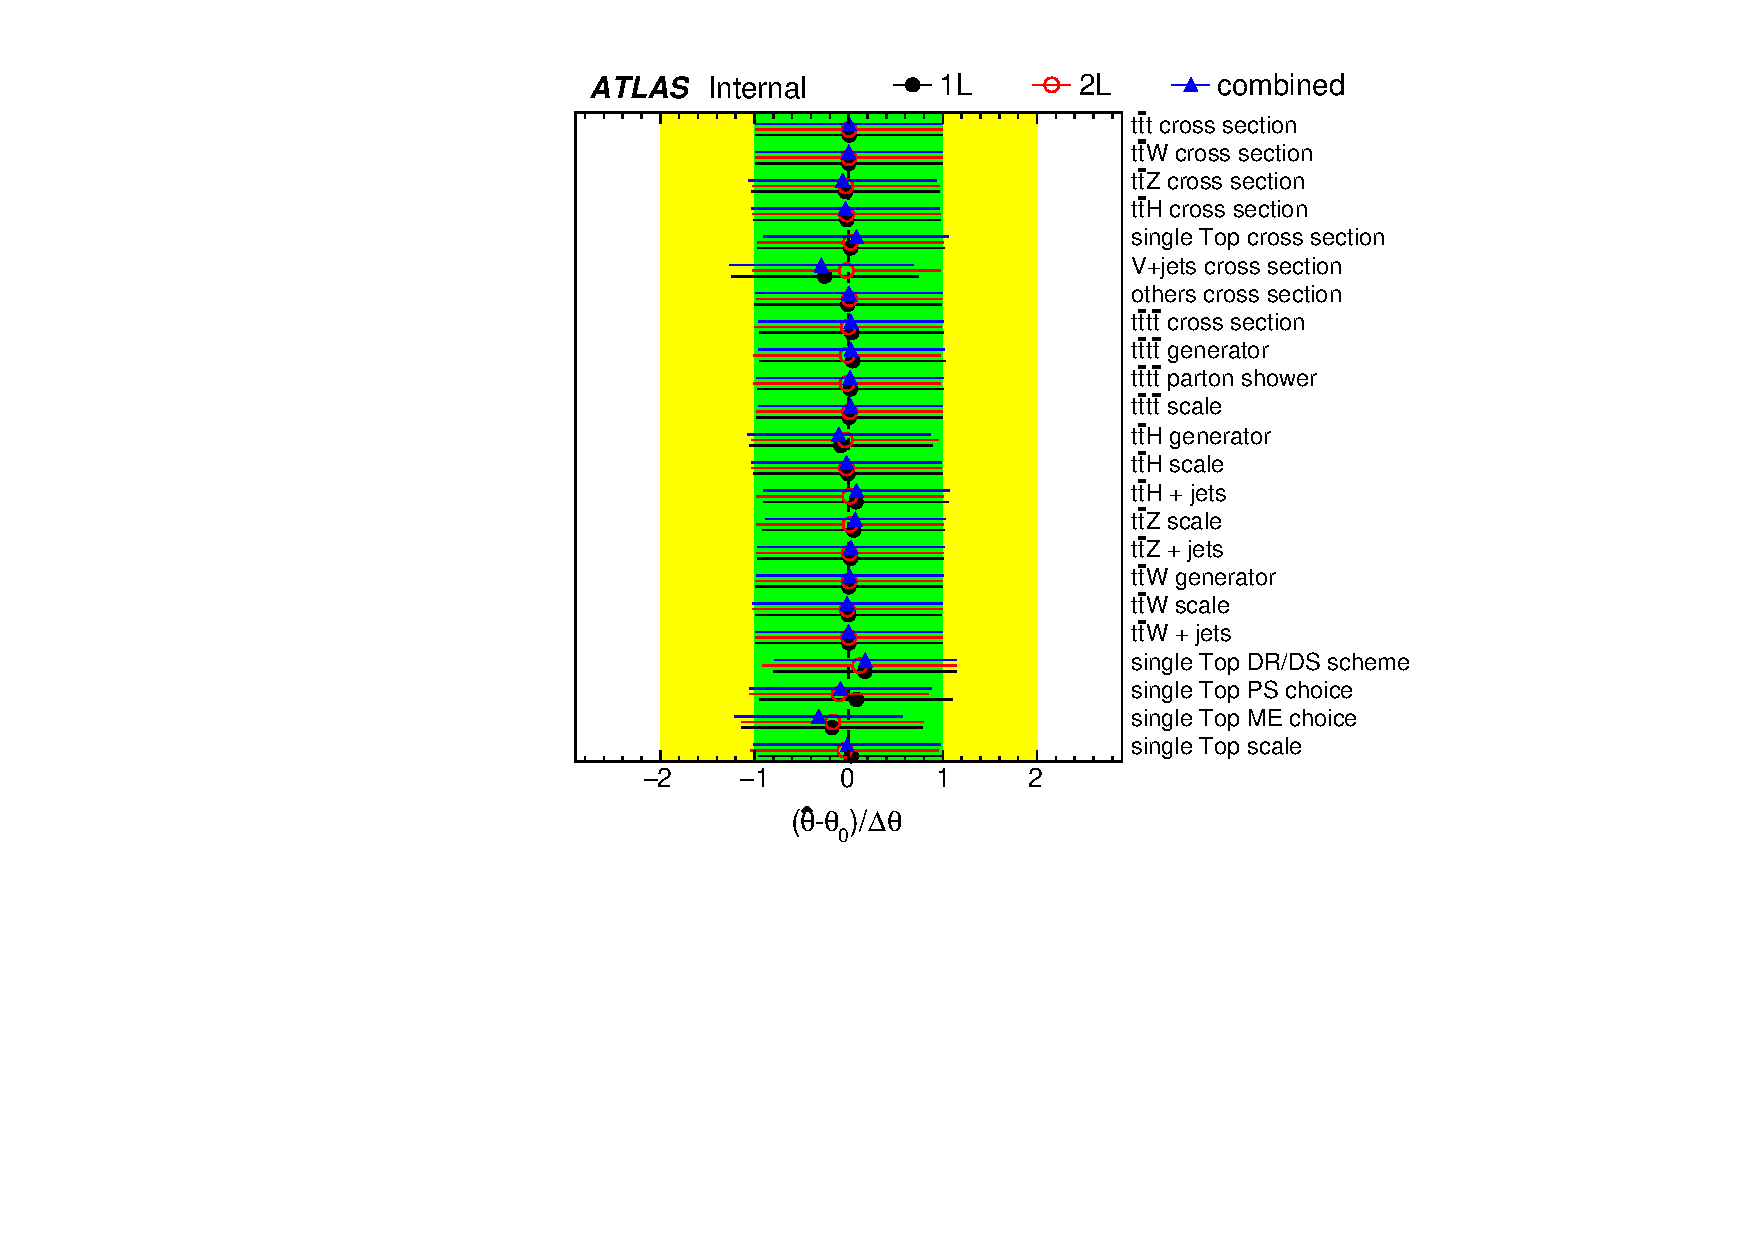
\includegraphics[width=\linewidth]{figures/fits/comparisons/selections/GNN/1000/data/NuisPar_comp_Other.pdf}
    \subcaption{mH=1000\gev}
    \label{fig:data_NP_mH400}
  \end{subfigure}
  \caption{\label{fig:data_NP_other}Fitted pulls and constraints for the  nuisance parameters corresponding to the non-\ttbar-background systematic uncertainties for the blinded Data fit for three mass points. Comparison is done for three fits: using only 1L regions, using only 2LOS regions and using all regions.}
\end{figure}



\begin{figure}[htbp!]
  \centering
  \begin{subfigure}[t]{0.32\textwidth}
    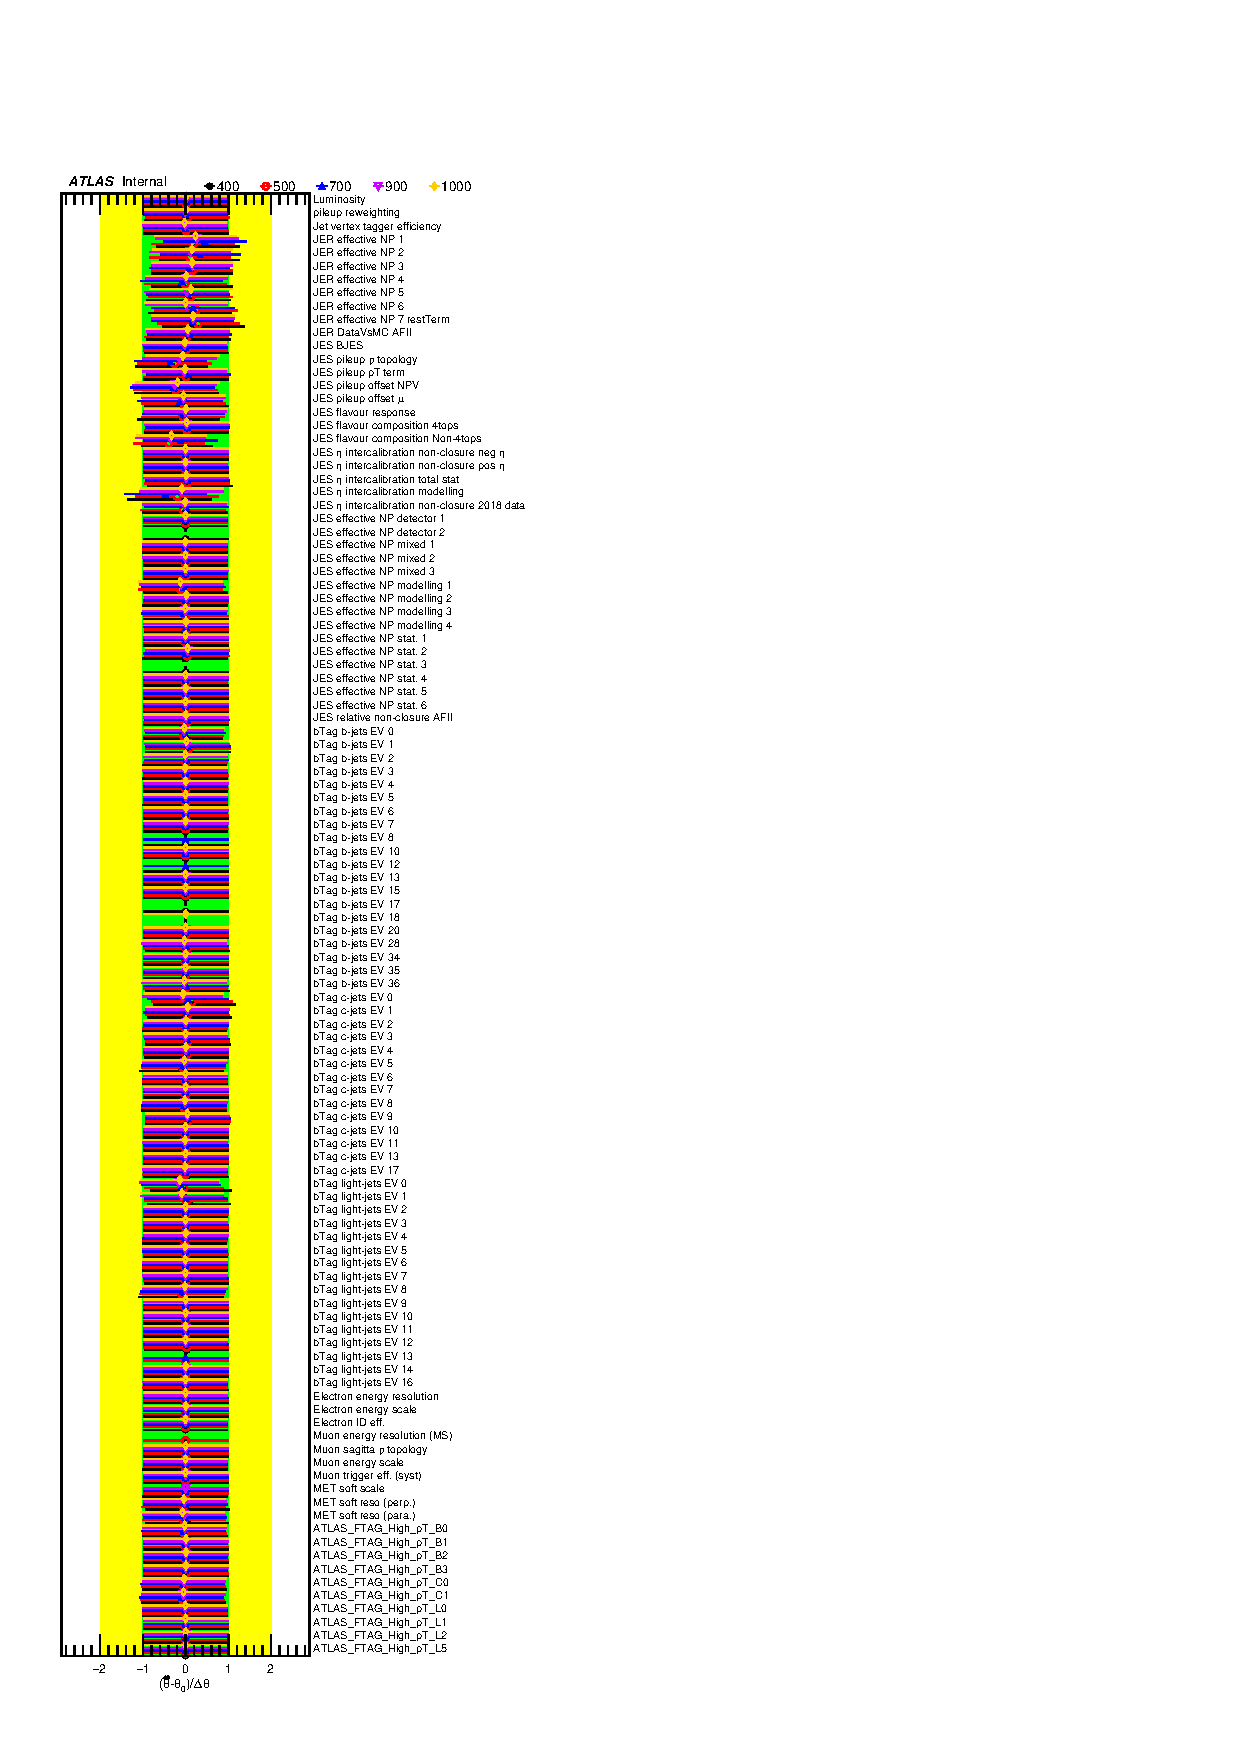
\includegraphics[width=\linewidth]{figures/fits/comparisons/massPoints/GNN/1L/data/NuisPar_comp_Instrumental.pdf}
    \subcaption{1L}
    \label{fig:data_NP_1L_instrumental}
  \end{subfigure}
  \begin{subfigure}[t]{0.32\textwidth}
    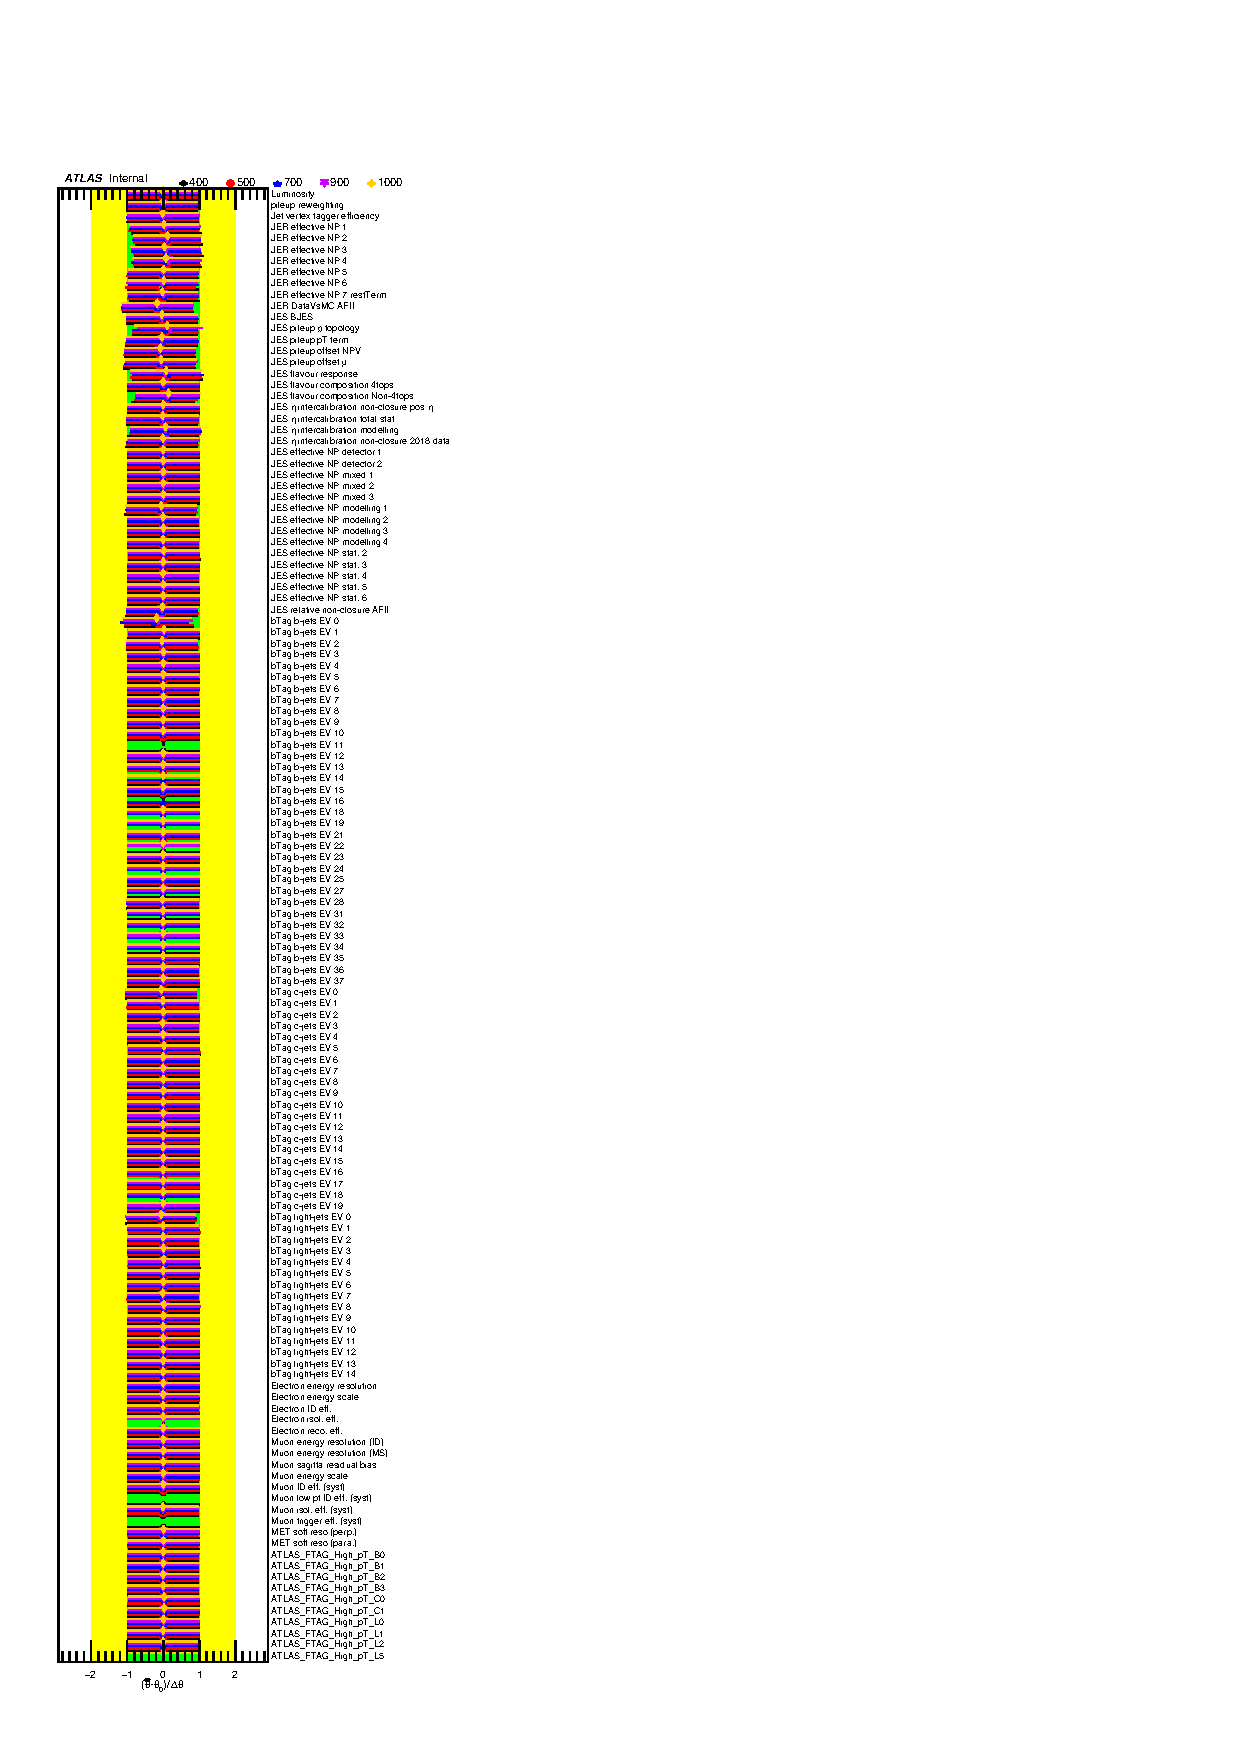
\includegraphics[width=\linewidth]{figures/fits/comparisons/massPoints/GNN/2L/data/NuisPar_comp_Instrumental.pdf}
    \subcaption{2L}
    \label{fig:data_NP_2L_instrumental}
  \end{subfigure}
  \begin{subfigure}[t]{0.32\textwidth}
    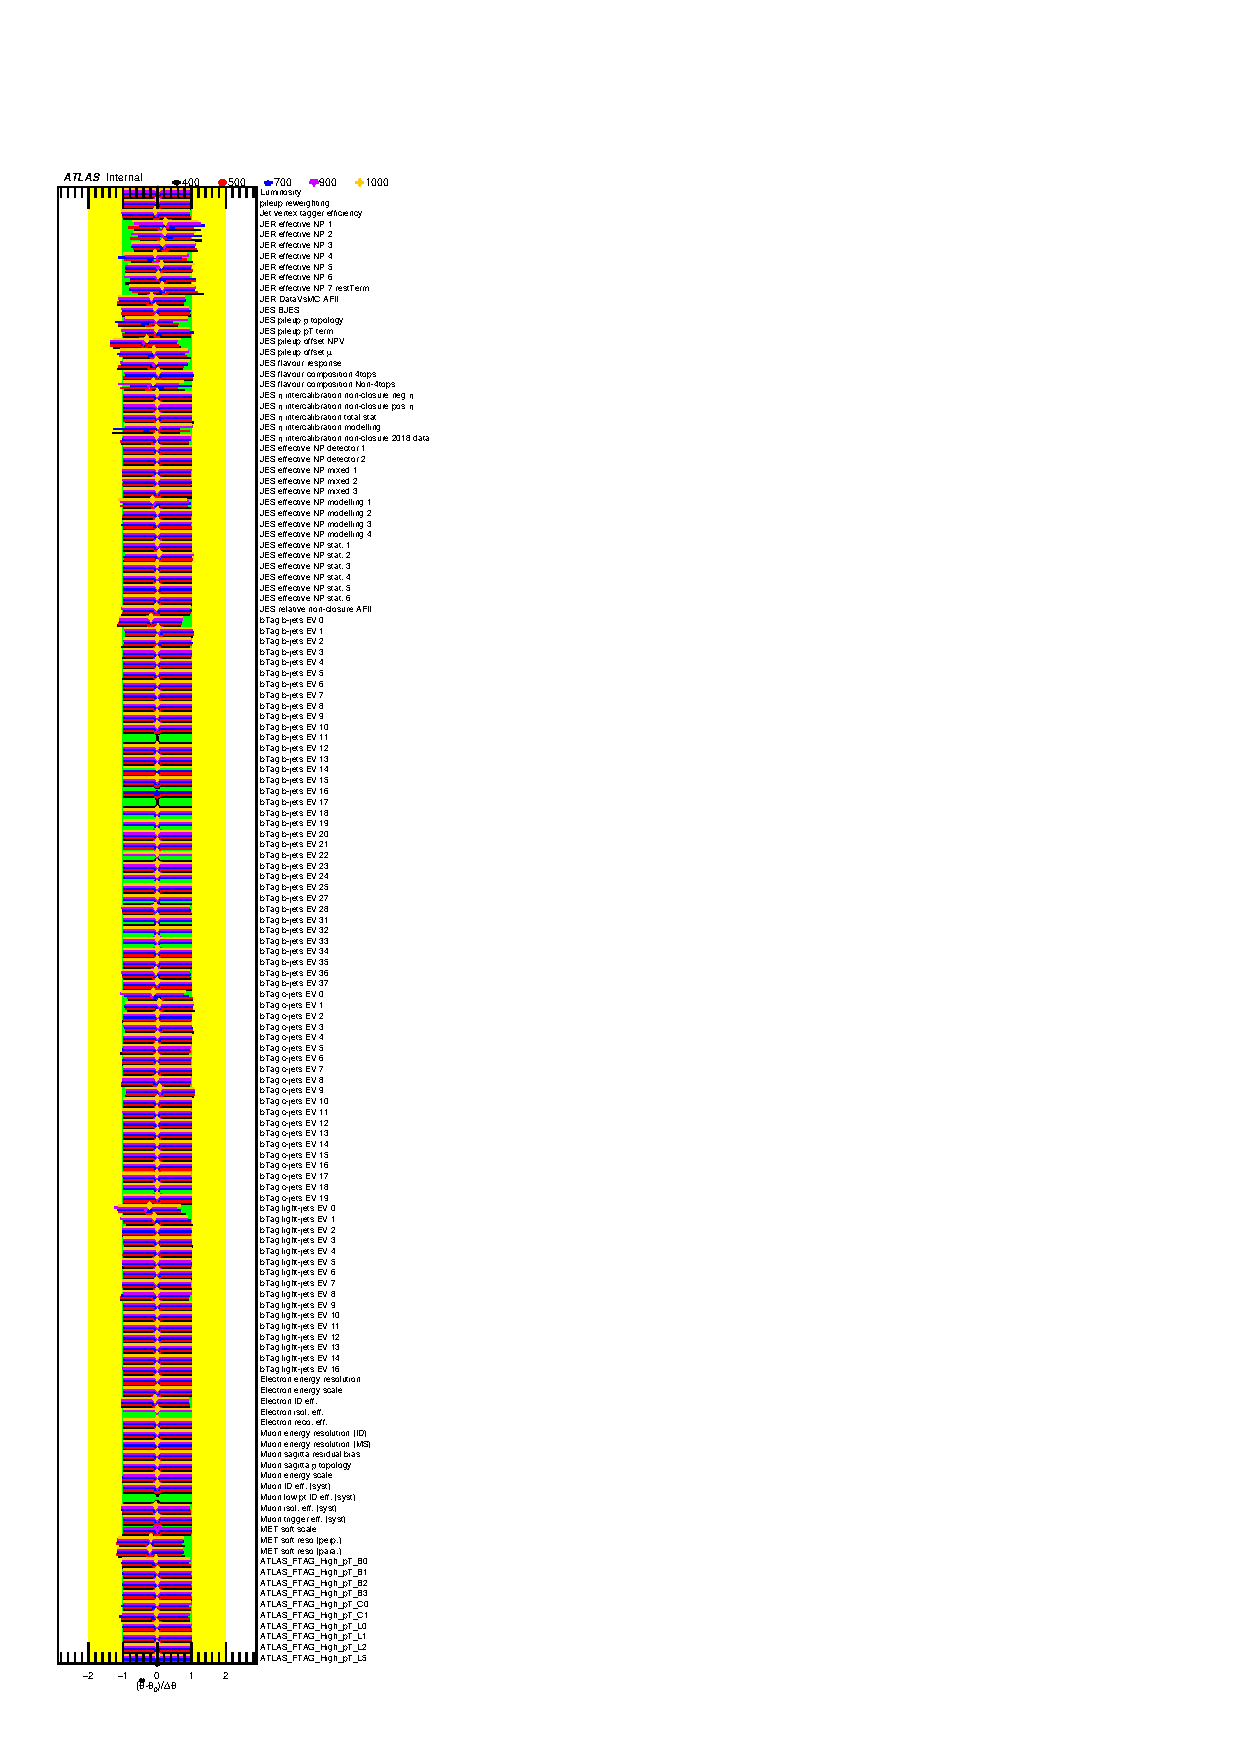
\includegraphics[width=\linewidth]{figures/fits/comparisons/massPoints/GNN/all/data/NuisPar_comp_Instrumental.pdf}
    \subcaption{1L+2L}
    \label{fig:data_NP_all_instrumental}
  \end{subfigure}
  \caption{Fitted pulls and constraints for the nuisance parameters corresponding to the instrumental systematic uncertainties for the blinded Data fit for three types of fits: using only 1L regions, using only 2L regions, and using all regions. Comparison is done for five mass points.}
\label{fig:data_NP_mass_instrumental}
\end{figure}


\begin{figure}[htbp!]
  \centering
  \begin{subfigure}[t]{0.32\textwidth}
    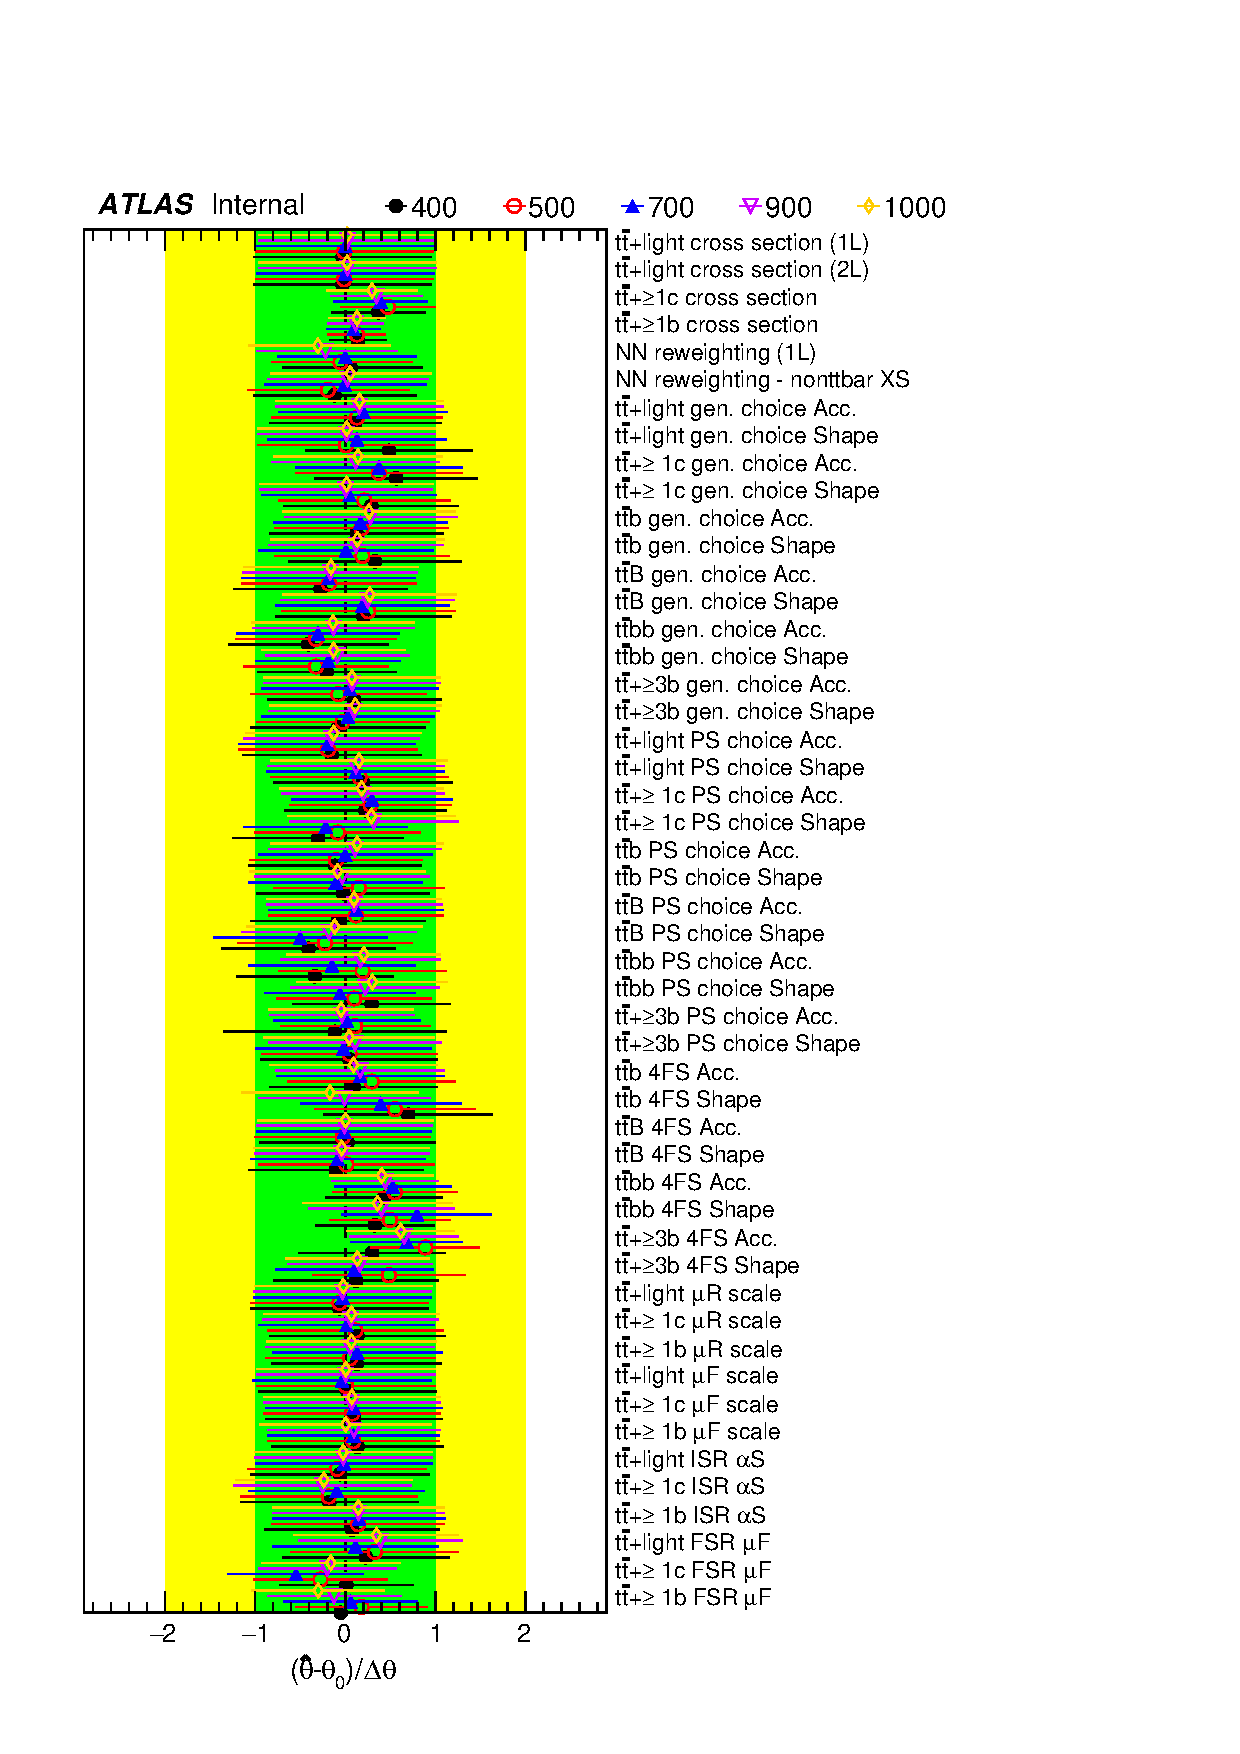
\includegraphics[width=\linewidth]{figures/fits/comparisons/massPoints/GNN/1L/data/NuisPar_comp_ttbar.pdf}
    \subcaption{1L}
    \label{fig:data_NP_1L}
  \end{subfigure}
  \begin{subfigure}[t]{0.32\textwidth}
    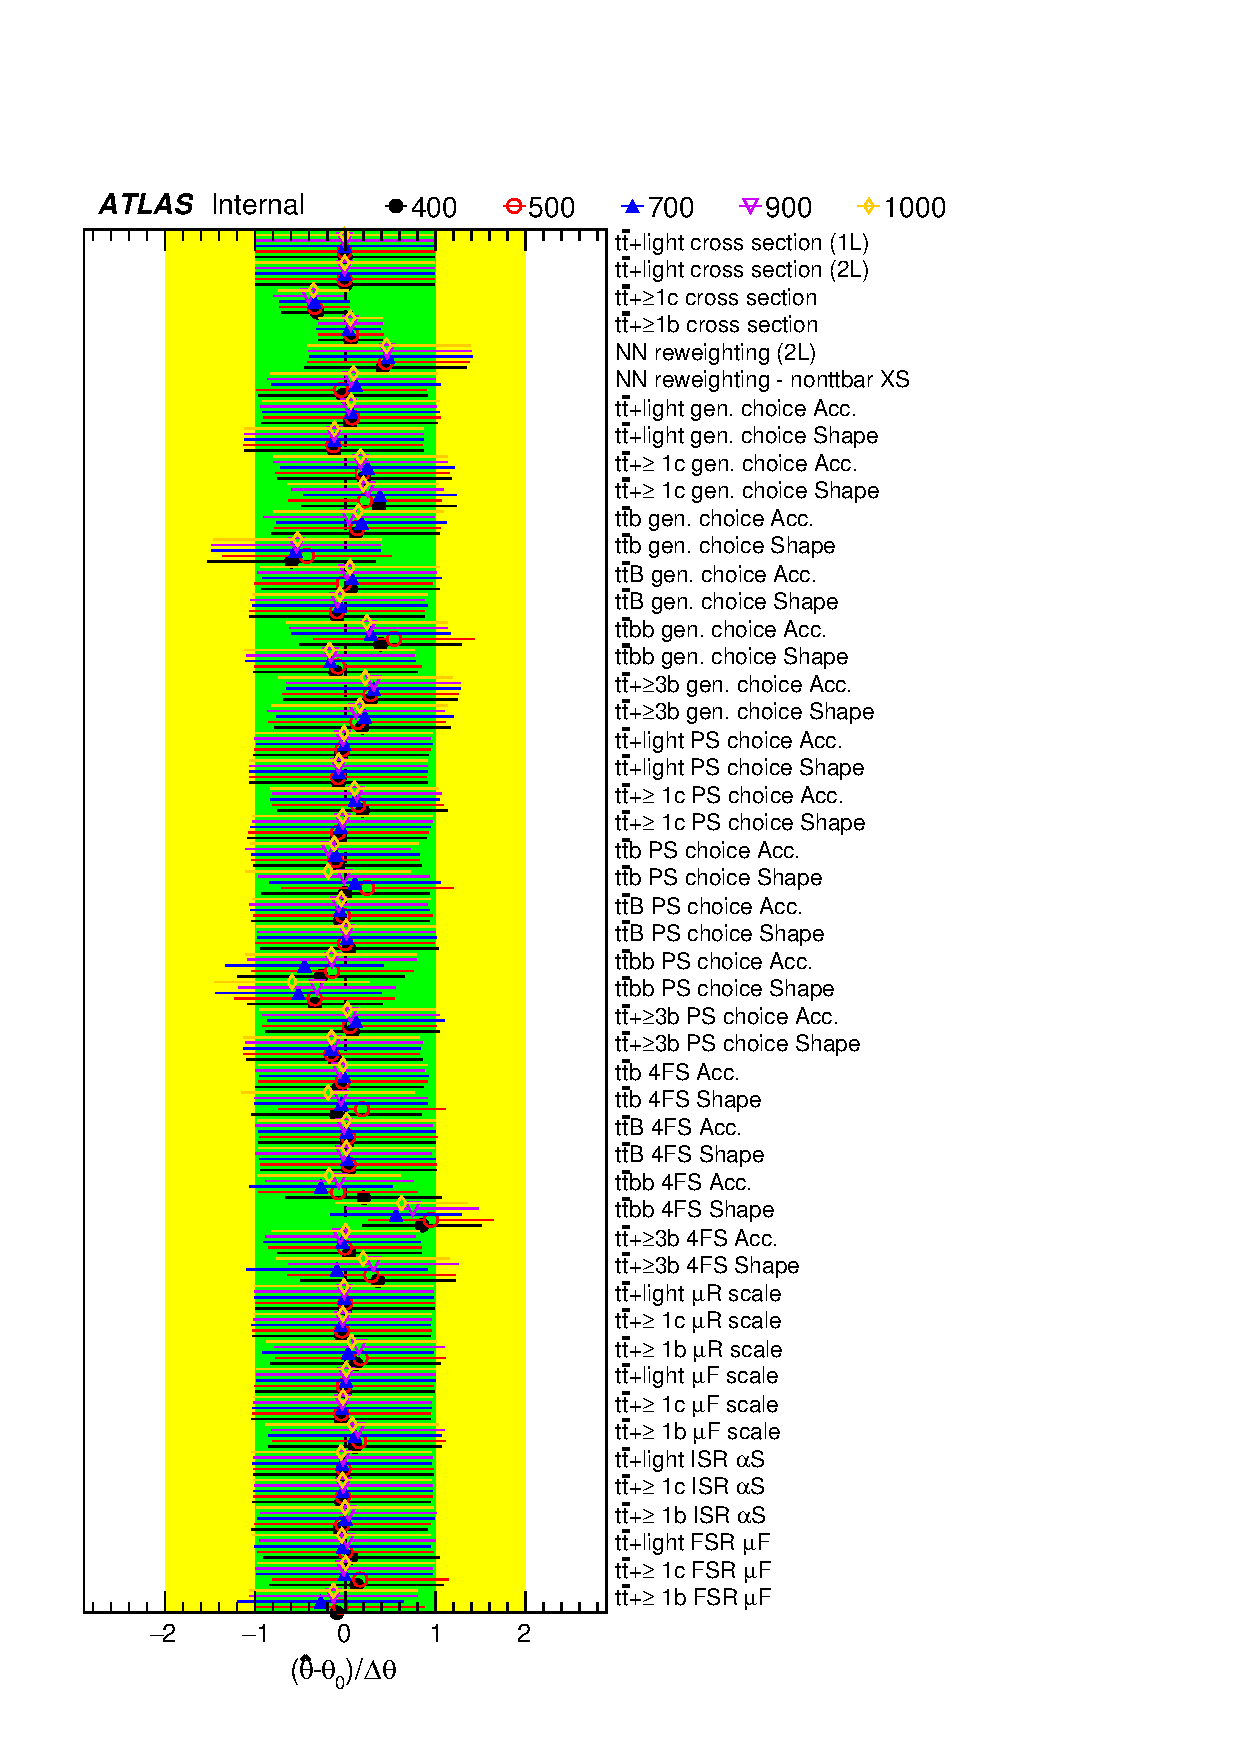
\includegraphics[width=\linewidth]{figures/fits/comparisons/massPoints/GNN/2L/data/NuisPar_comp_ttbar.pdf}
    \subcaption{2L}
    \label{fig:data_NP_2L}
  \end{subfigure}
  \begin{subfigure}[t]{0.32\textwidth}
    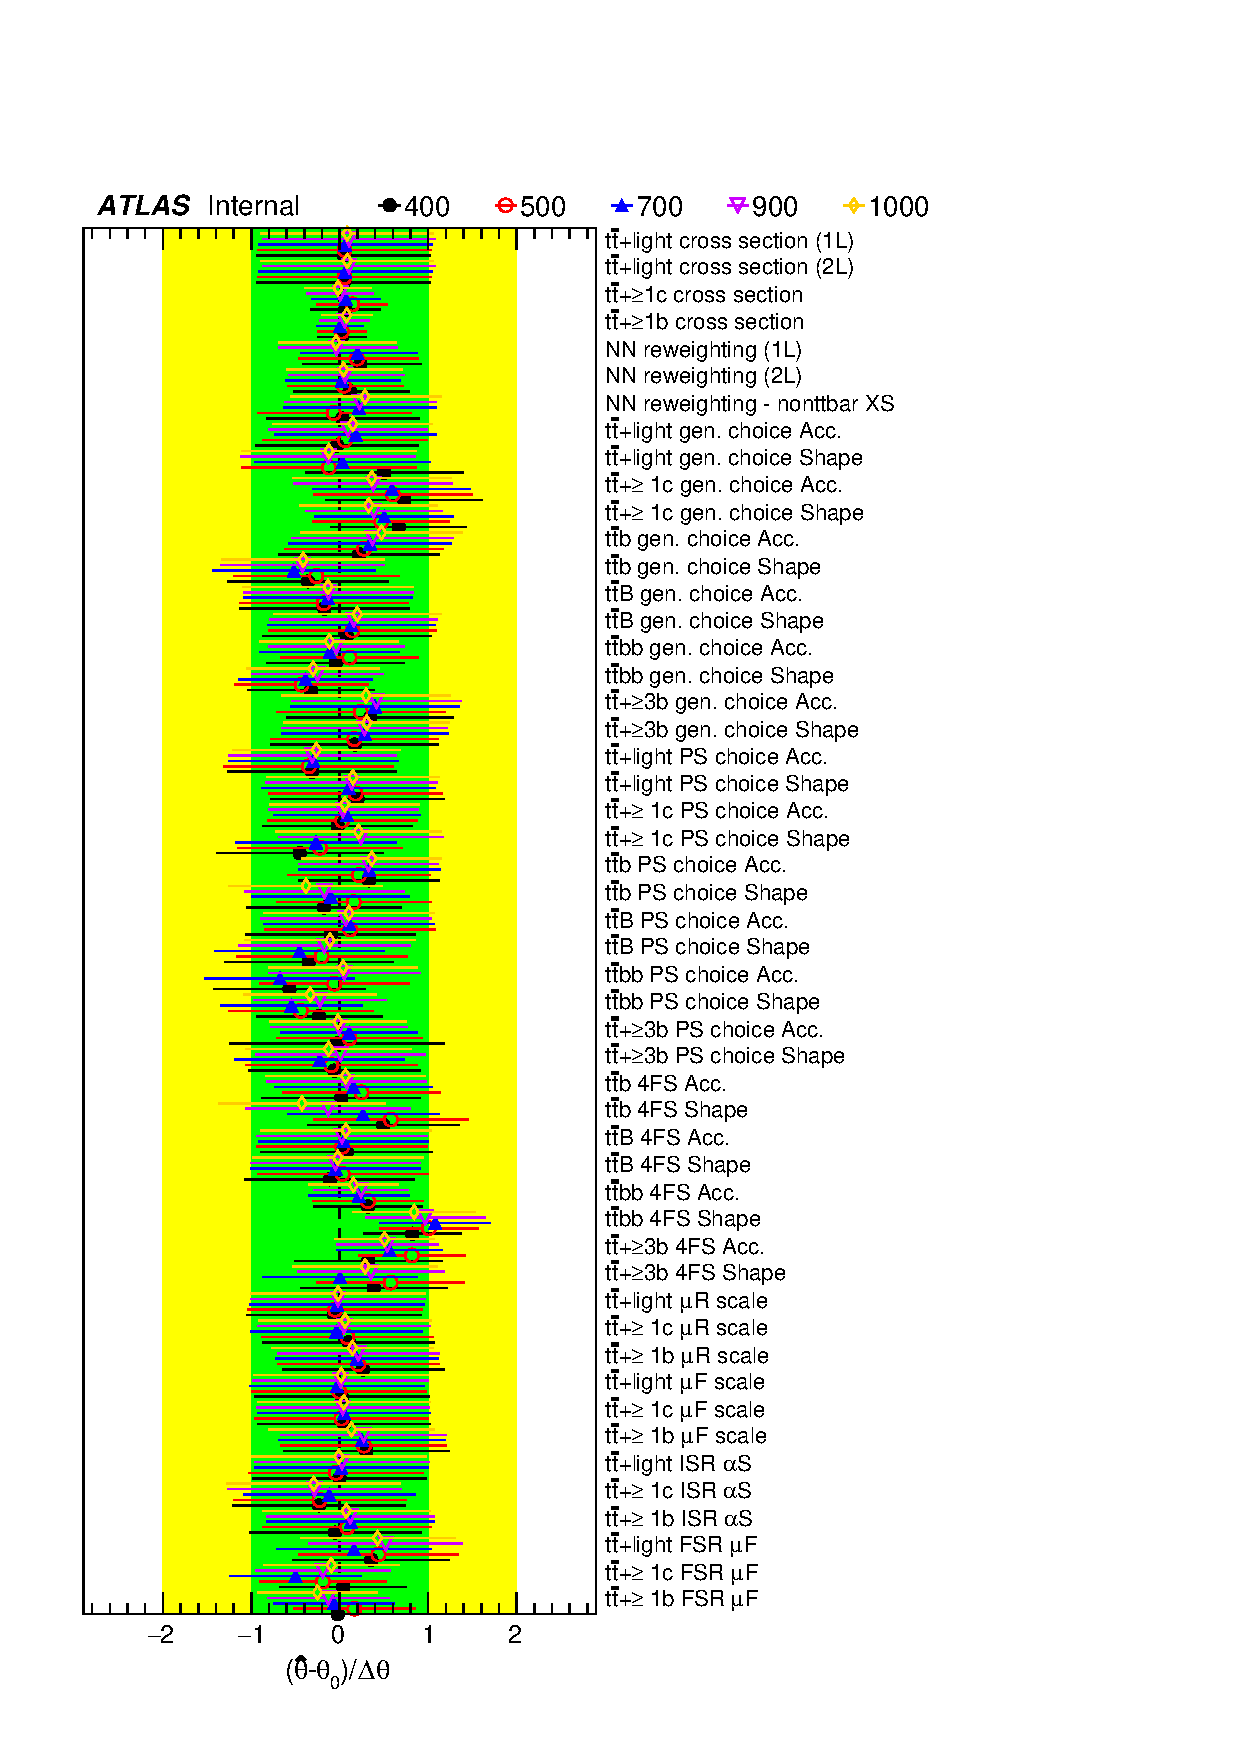
\includegraphics[width=\linewidth]{figures/fits/comparisons/massPoints/GNN/all/data/NuisPar_comp_ttbar.pdf}
    \subcaption{1L+2L}
    \label{fig:data_NP_all}
  \end{subfigure}
  \caption{Fitted pulls and constraints for the nuisance parameters corresponding to the \ttbar systematic uncertainties for the blinded Data fit for three types of fits: using only 1L regions, using only 2L regions, and using all regions. Comparison is done for five mass points.}
\label{fig:data_NP_mass_ttbar}
\end{figure}


\begin{figure}[htbp!]
  \centering
  \begin{subfigure}[t]{0.32\textwidth}
    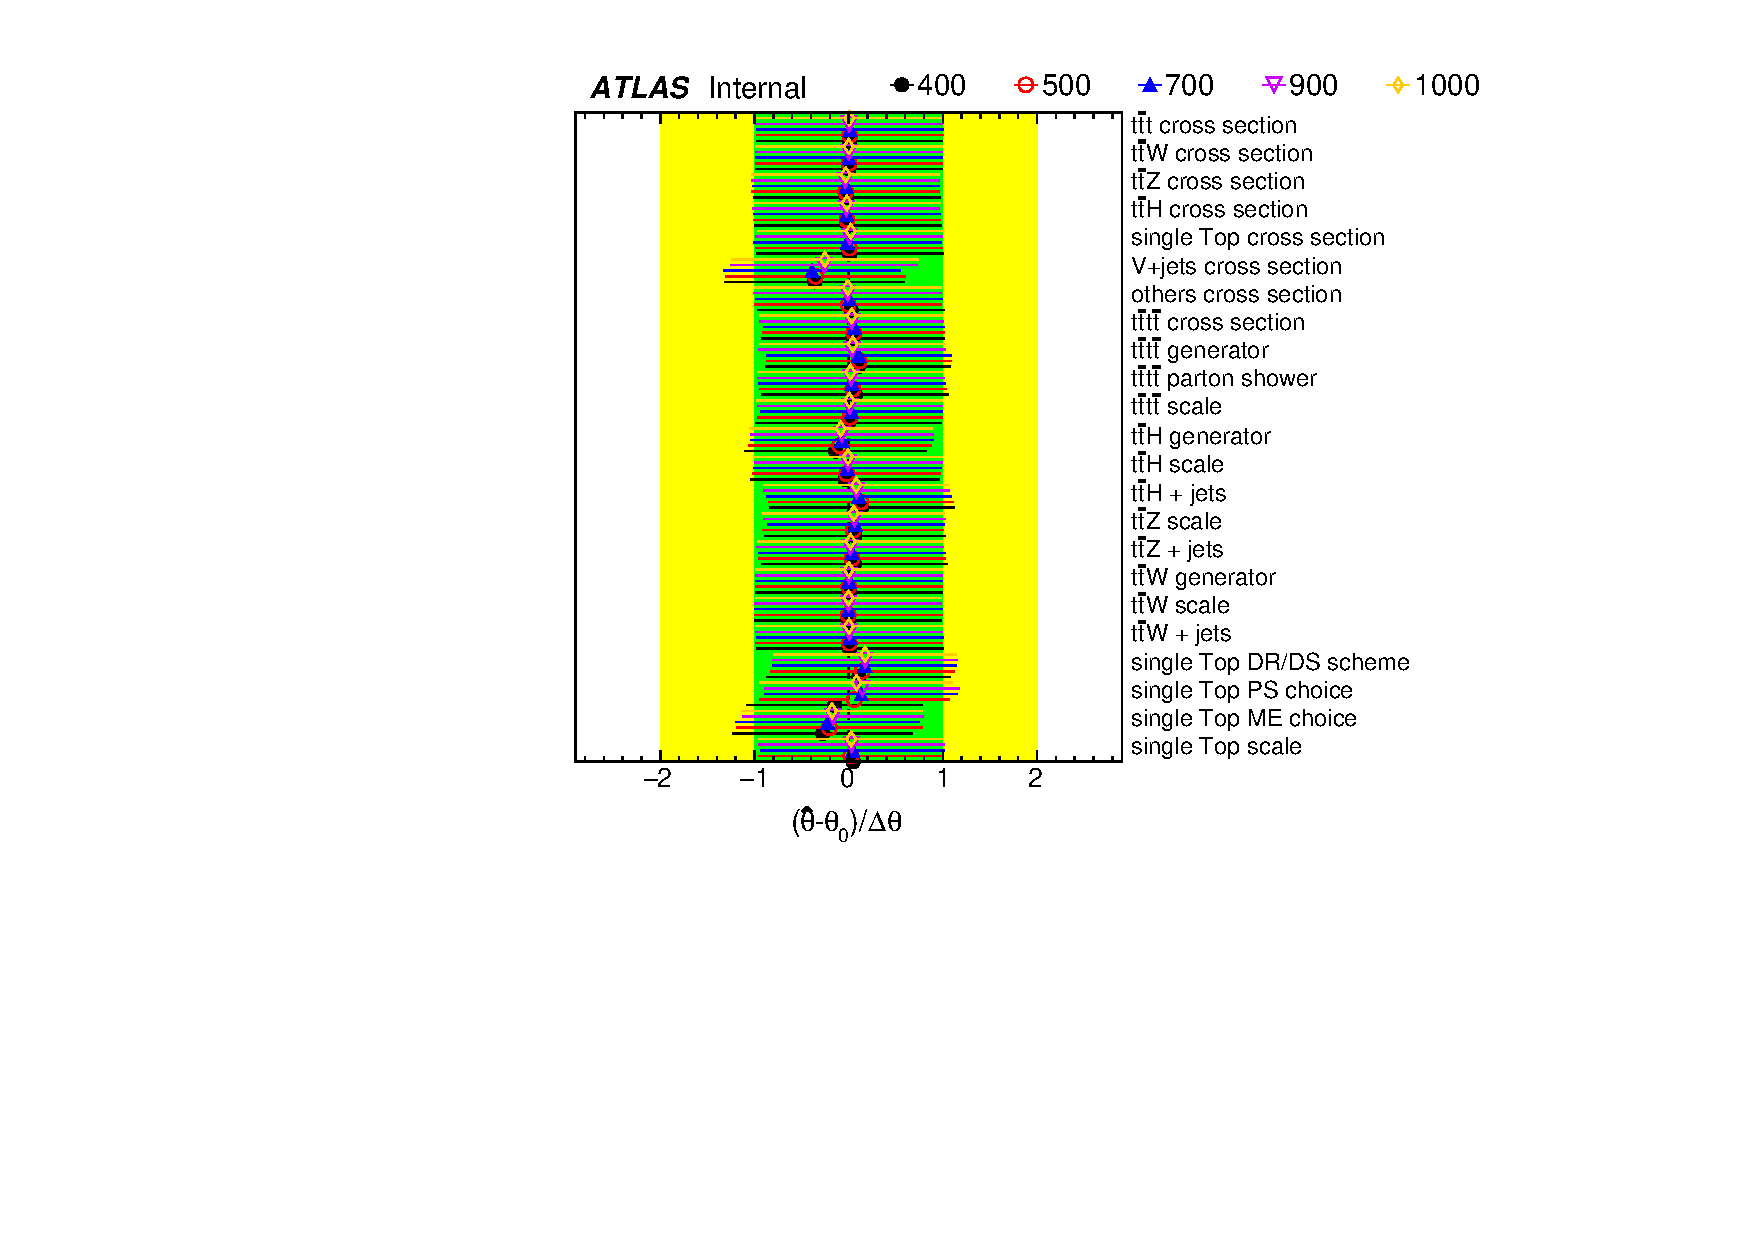
\includegraphics[width=\linewidth]{figures/fits/comparisons/massPoints/GNN/1L/data/NuisPar_comp_Other.pdf}
    \subcaption{1L}
    \label{fig:data_NP_1L_other}
  \end{subfigure}
  \begin{subfigure}[t]{0.32\textwidth}
    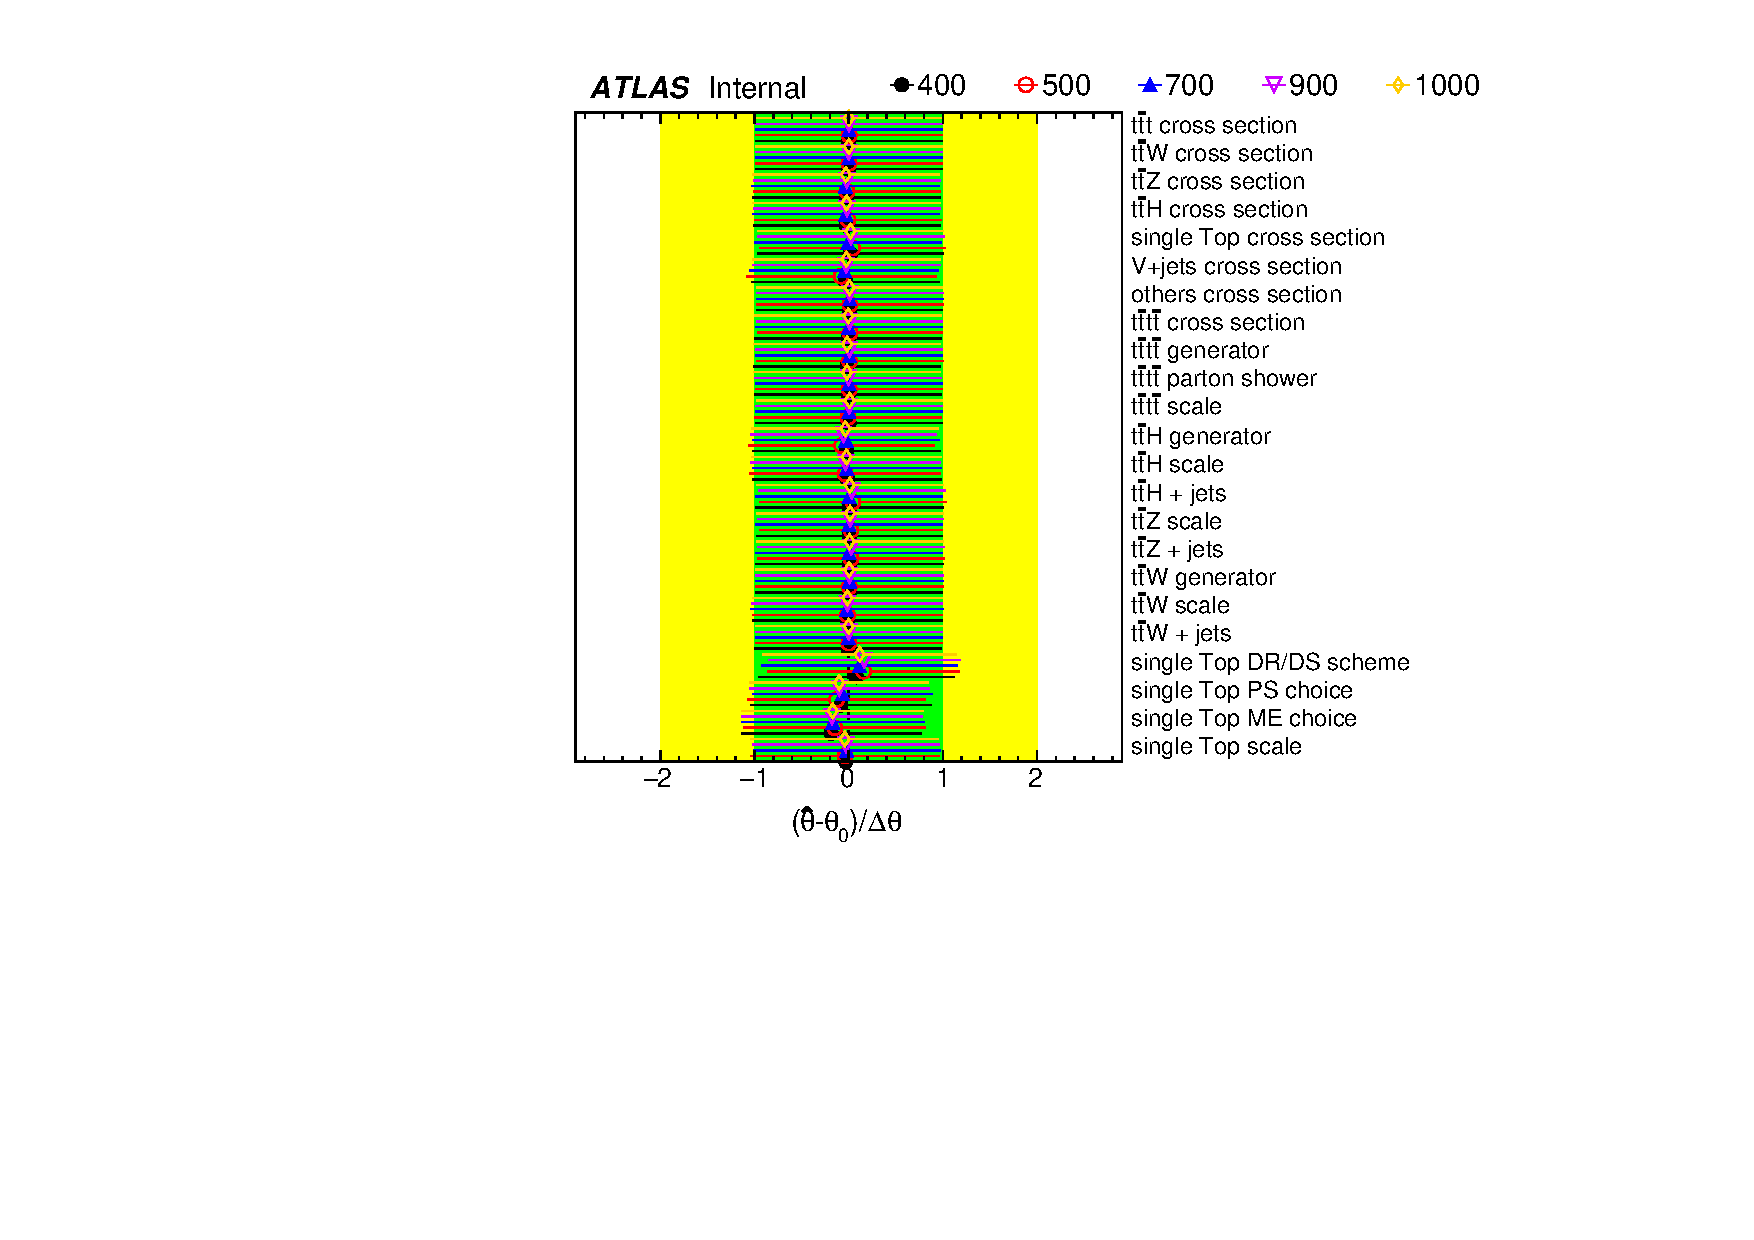
\includegraphics[width=\linewidth]{figures/fits/comparisons/massPoints/GNN/2L/data/NuisPar_comp_Other.pdf}
    \subcaption{2L}
    \label{fig:data_NP_2L_other}
  \end{subfigure}
  \begin{subfigure}[t]{0.32\textwidth}
    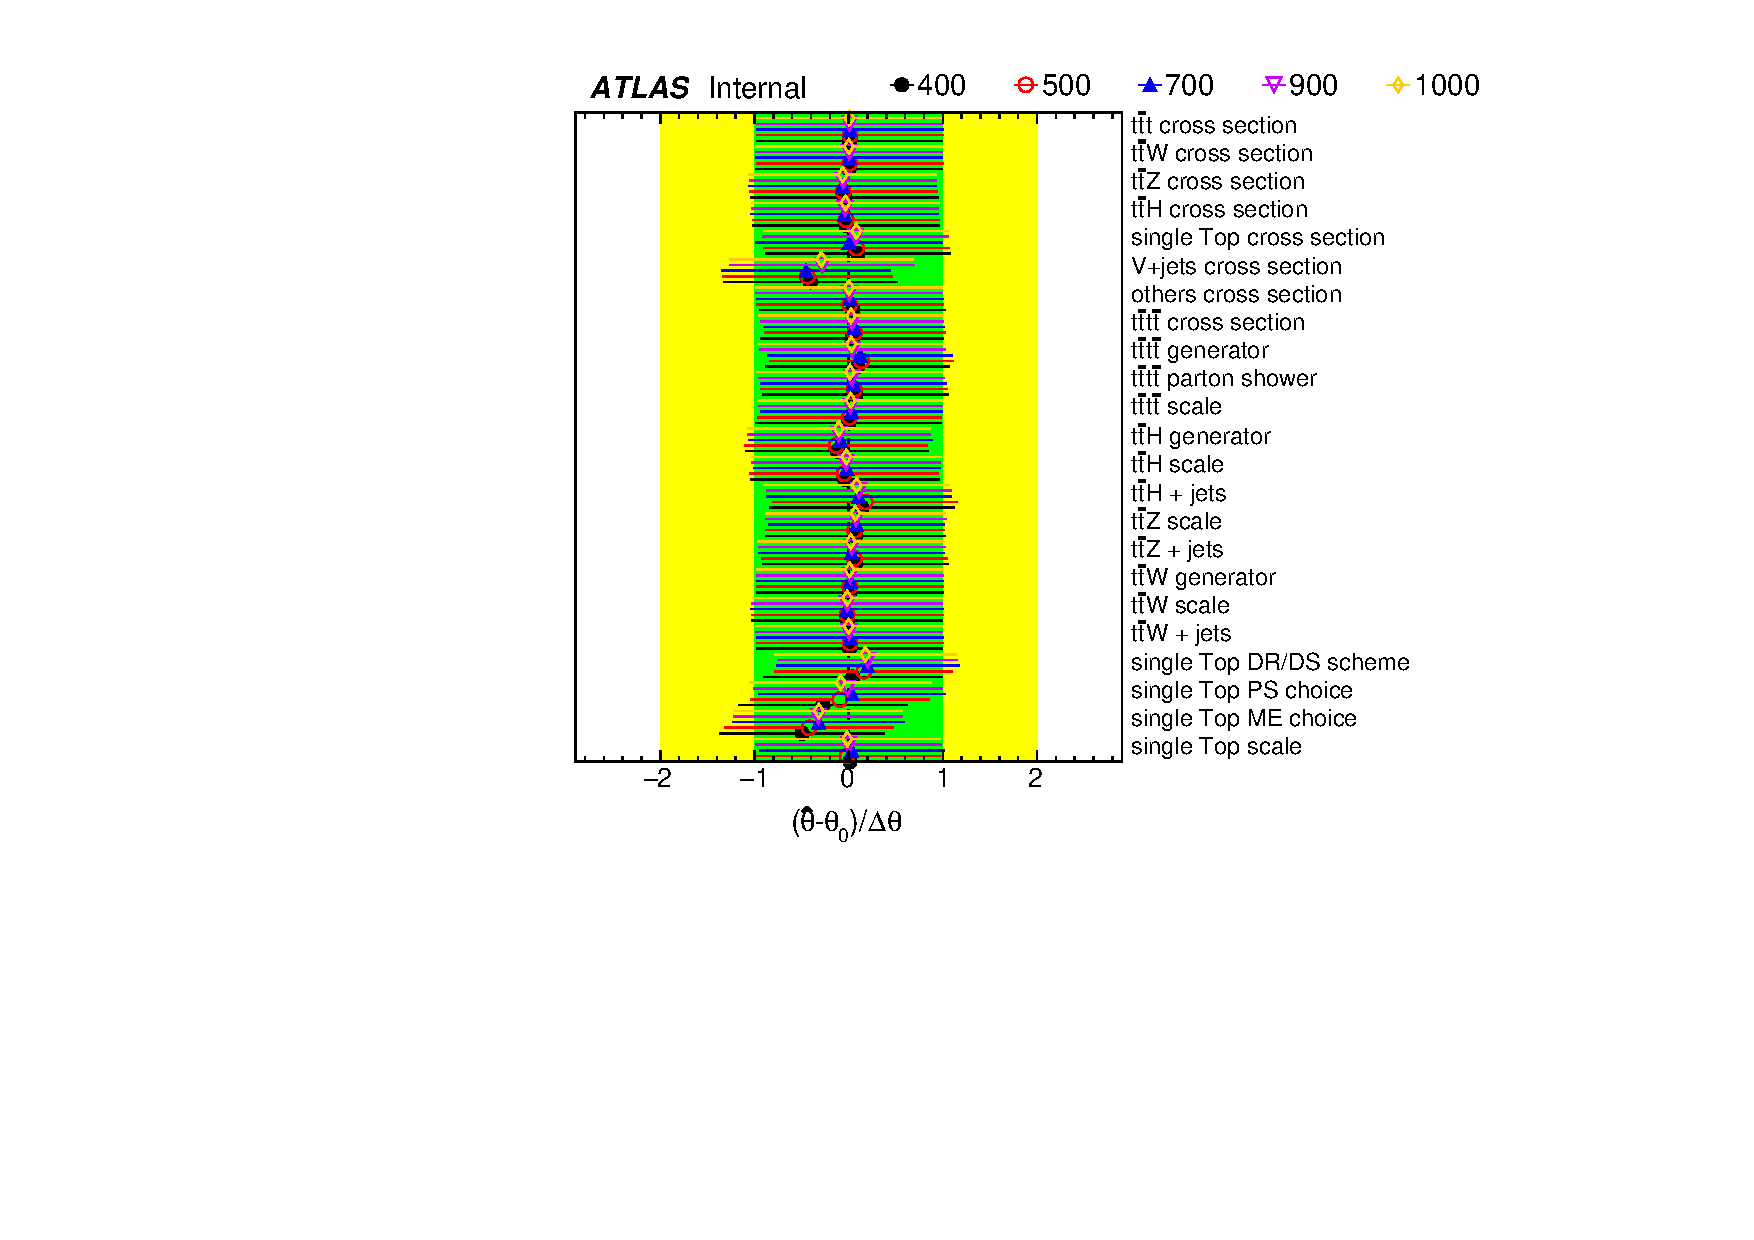
\includegraphics[width=\linewidth]{figures/fits/comparisons/massPoints/GNN/all/data/NuisPar_comp_Other.pdf}
    \subcaption{1L+2L}
    \label{fig:data_NP_all_other}
  \end{subfigure}
  \caption{Fitted pulls and constraints for the nuisance parameters corresponding to the non-\ttbar-background systematic uncertainties for the blinded Data fit for three types of fits: using only 1L regions, using only 2L regions, and using all regions. Comparison is done for five mass points.}
\label{fig:data_NP_mass_other}
\end{figure}


\begin{figure}[htbp!]
        \centering
        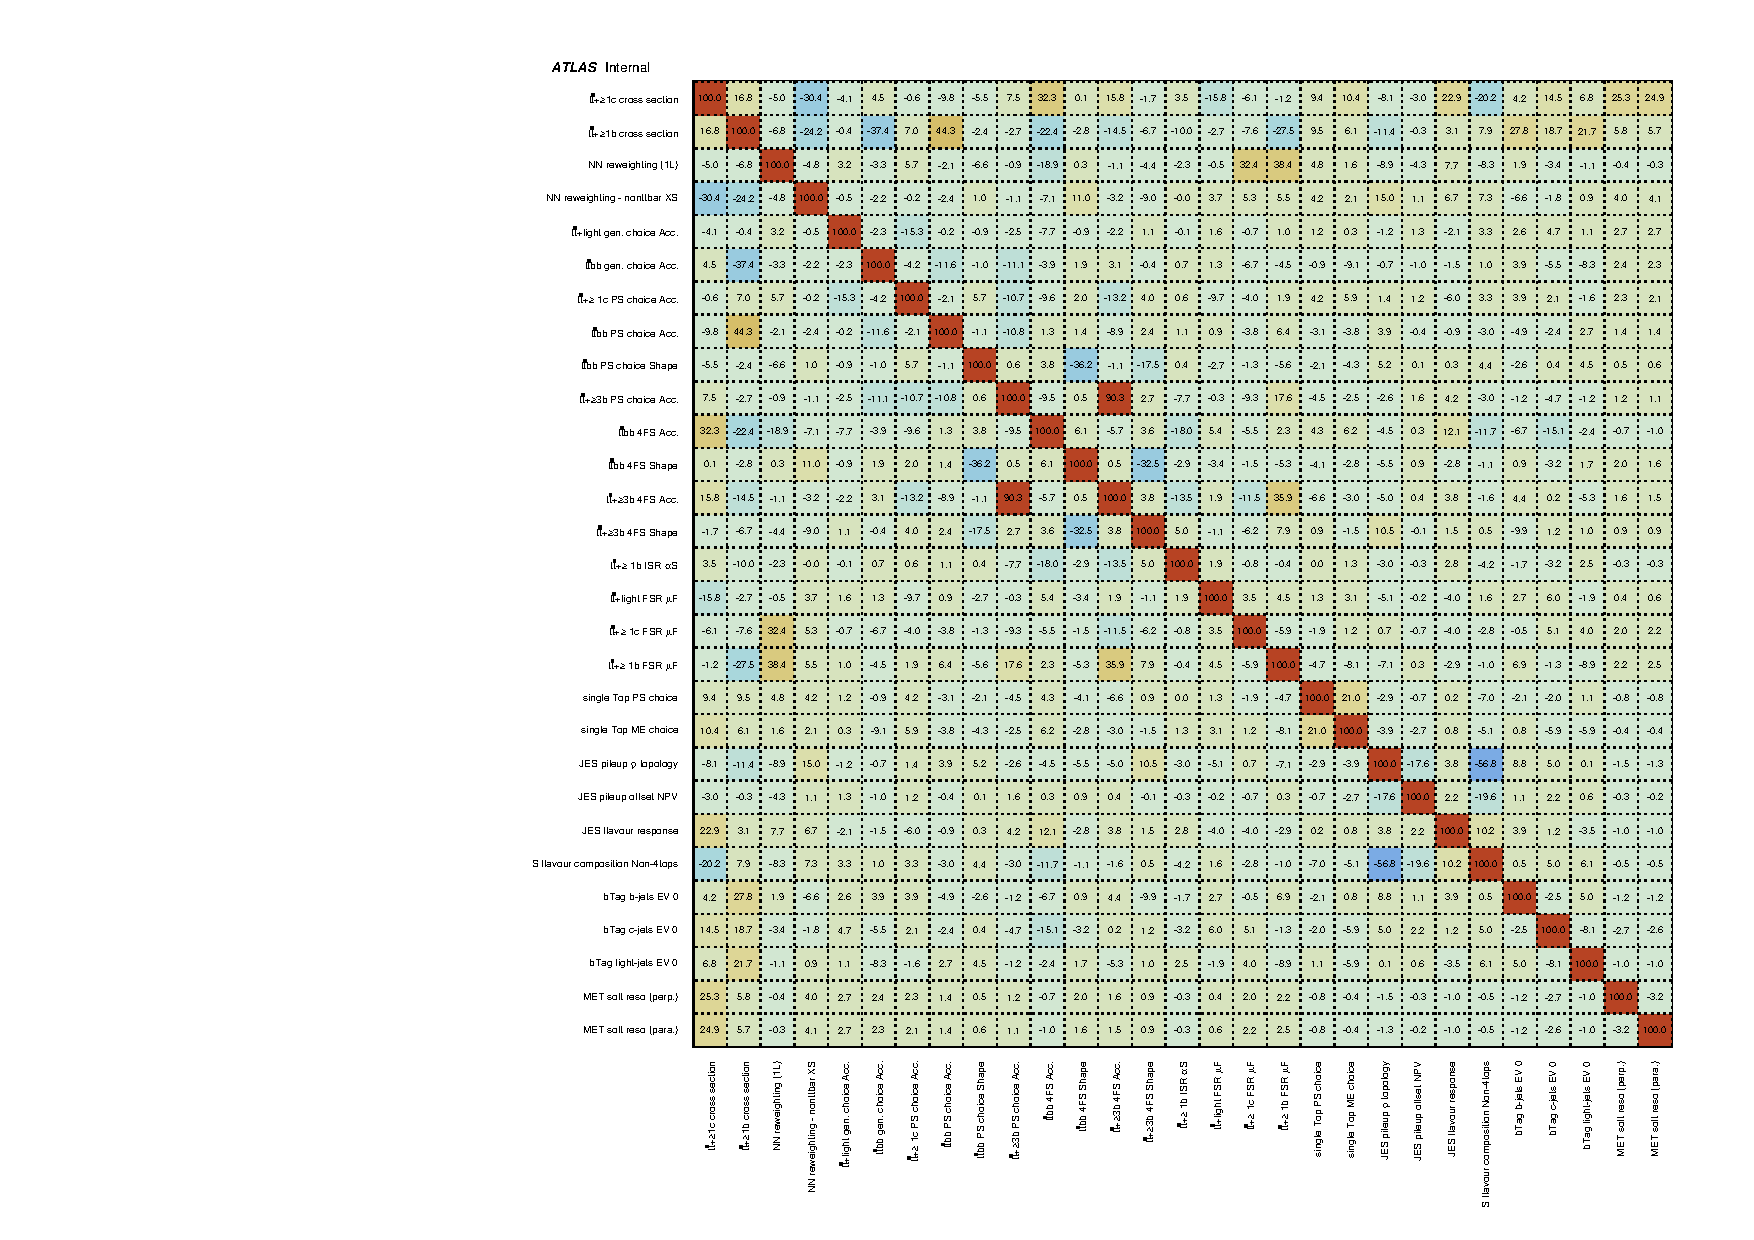
\includegraphics[width=\linewidth]{figures/fits/GNN/400/1L/data/CorrMatrix.pdf}
        \caption{\label{fig:Corr_mH400_Data_1L}Correlation matrix for the 1L blinded data fit for mH = 400 GeV}
\end{figure}

\begin{figure}[htbp!]
        \centering
        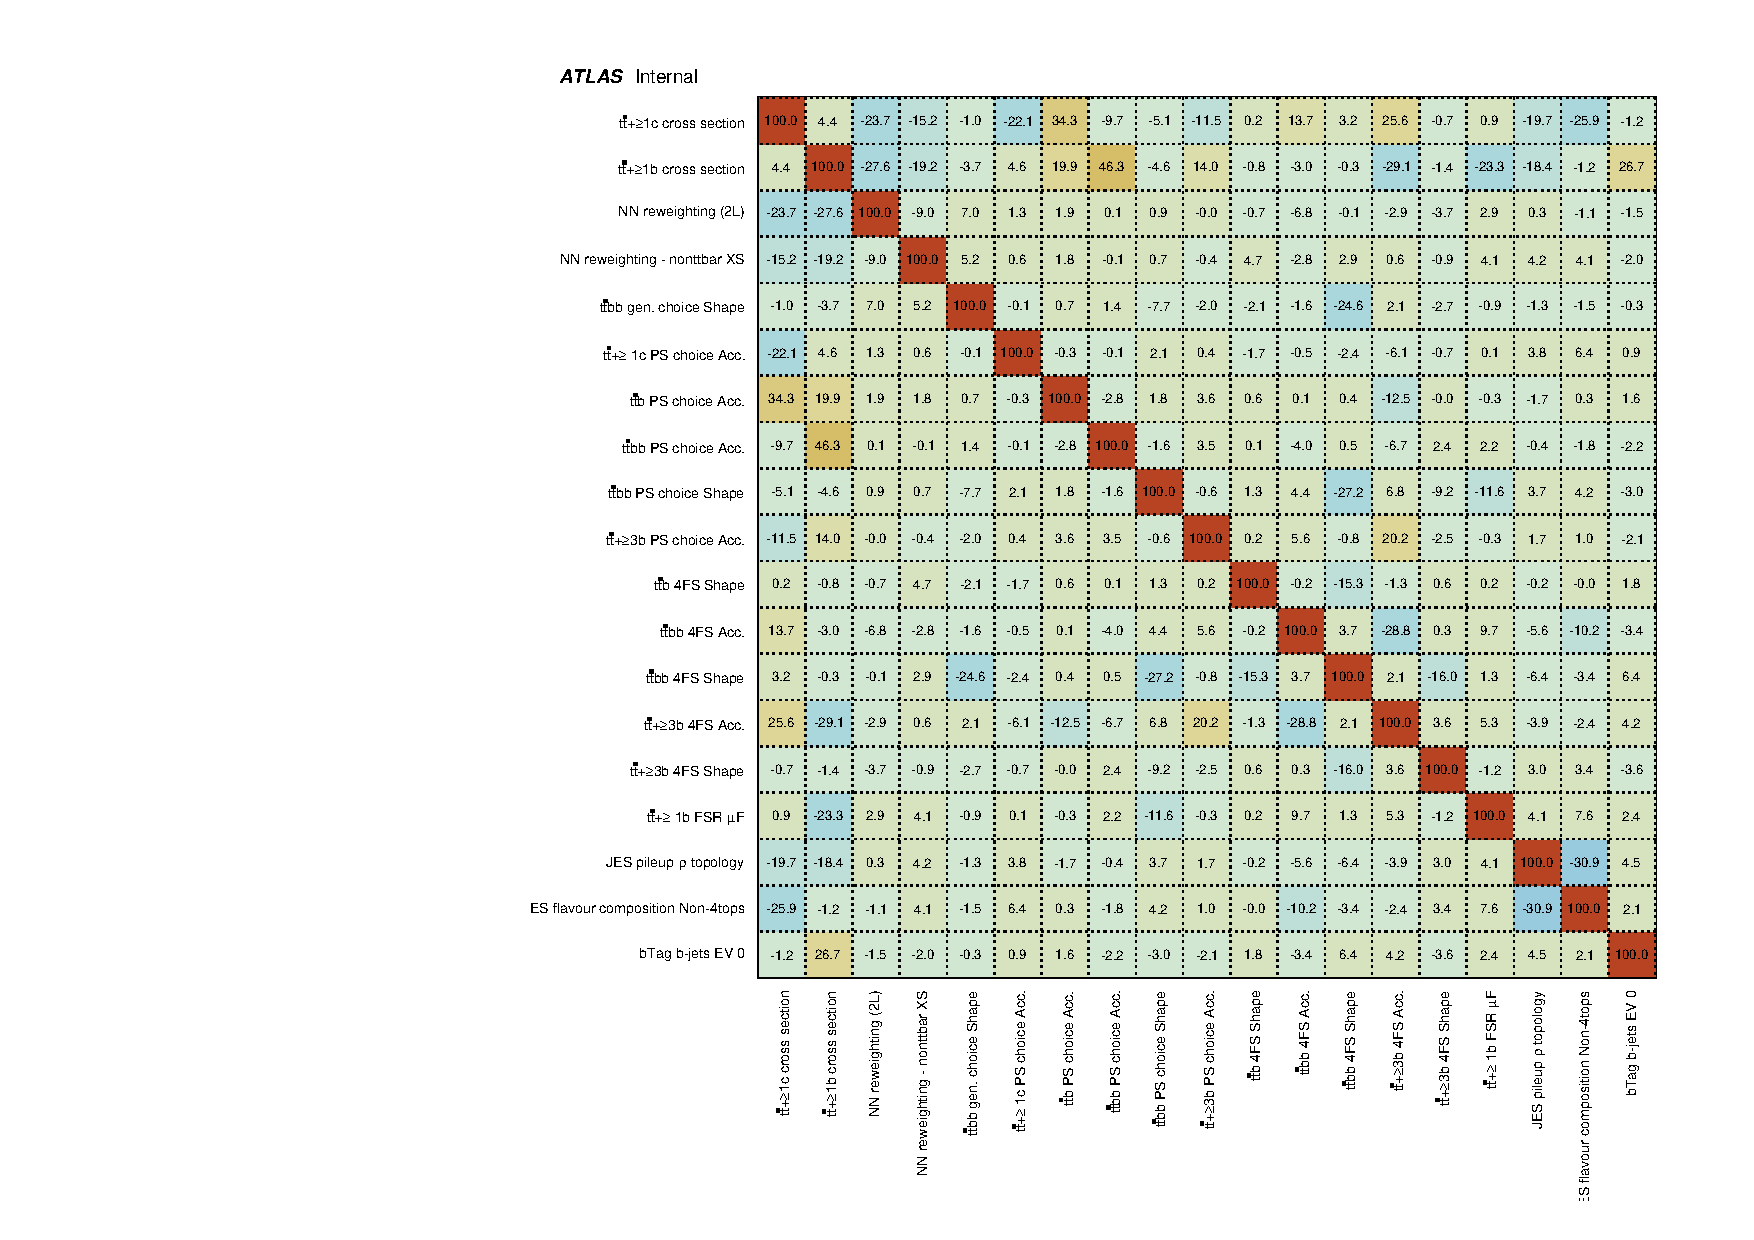
\includegraphics[width=\linewidth]{figures/fits/GNN/400/2L/data/CorrMatrix.pdf}
        \caption{\label{fig:Corr_mH400_Data_2L}Correlation matrix for the 2LOS blinded data fit for mH = 400 GeV}
\end{figure}

\begin{figure}[htbp!]
        \centering
        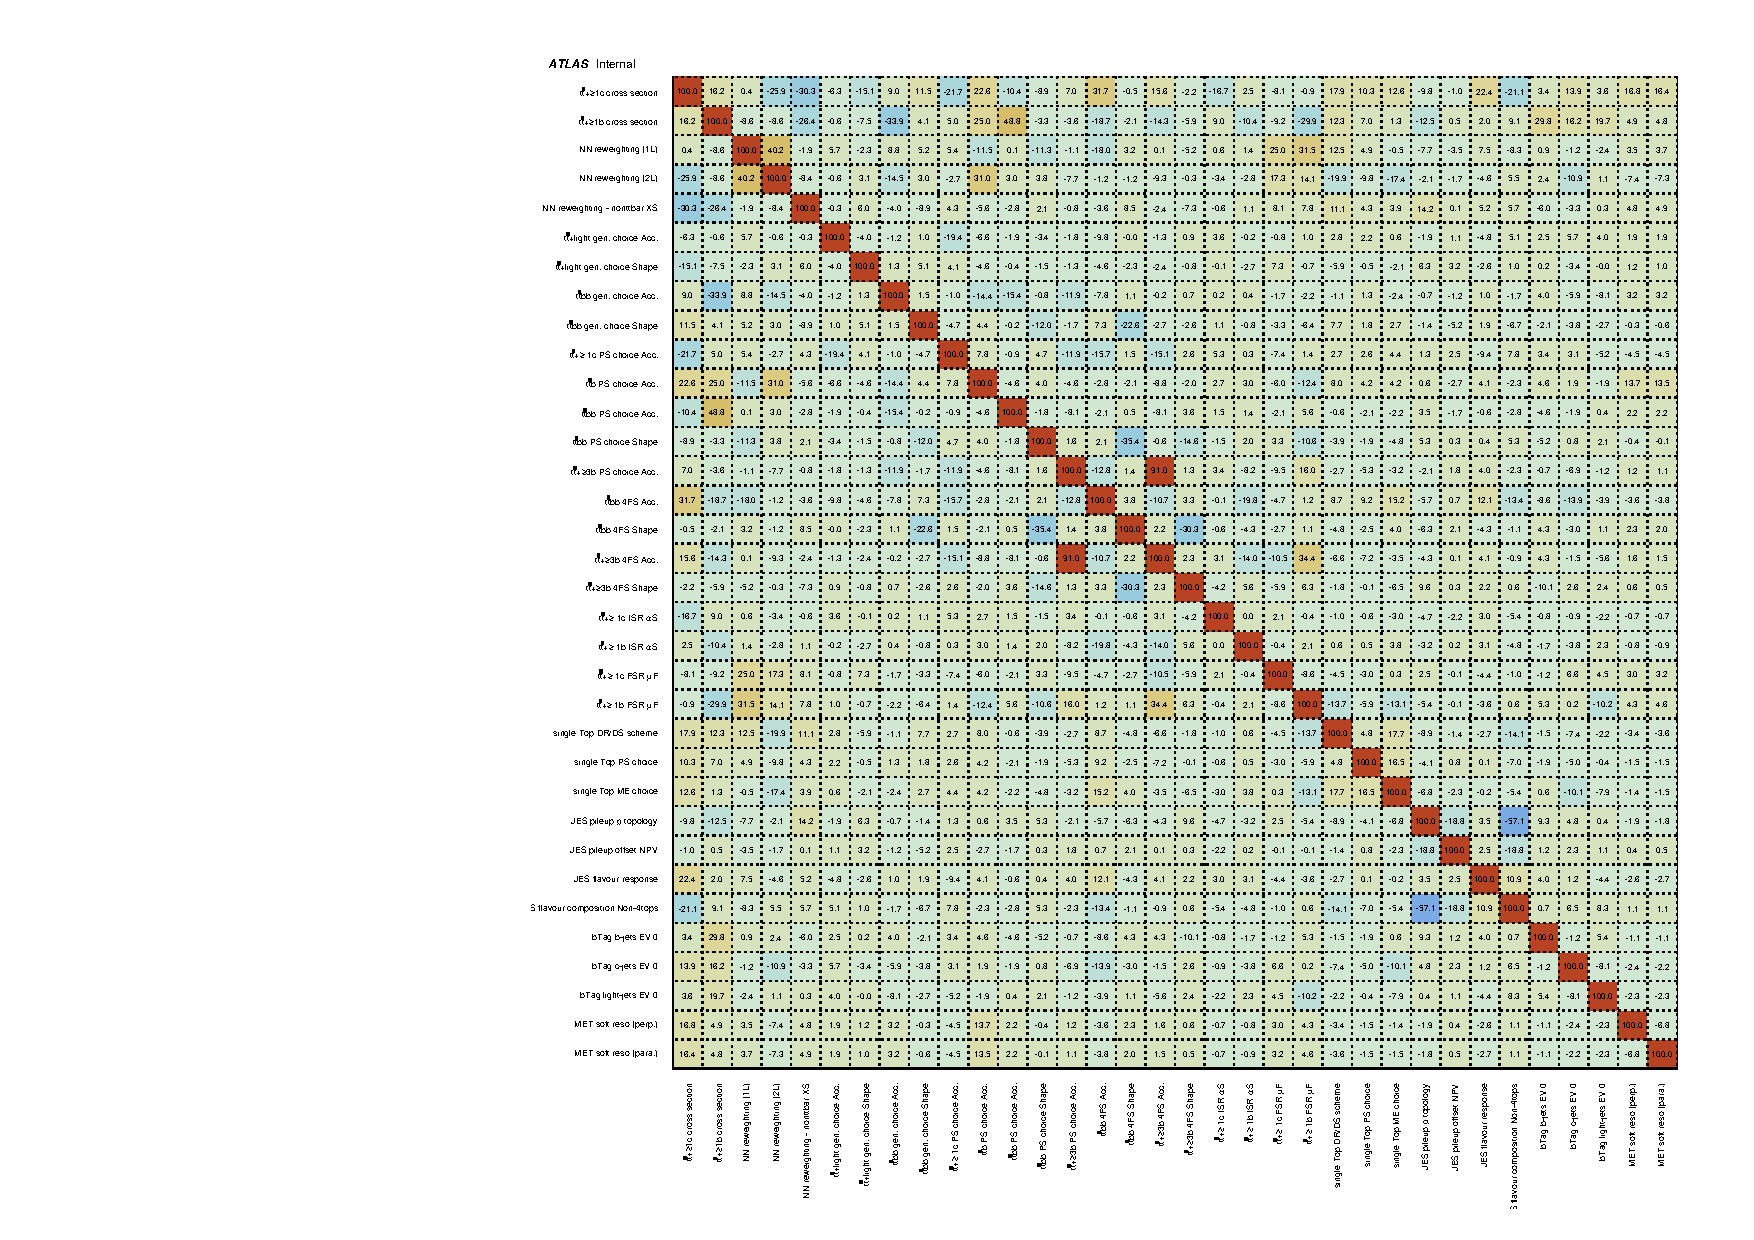
\includegraphics[width=\linewidth]{figures/fits/GNN/400/all/data/CorrMatrix.pdf}
        \caption{\label{fig:Corr_mH400_Data_all}Correlation matrix for the 1L/2LOS combined blinded data fit for mH = 400 GeV}
\end{figure}
